\chapter{基于贝叶斯自监督对比损失的推荐算法研究}
\label{cha:fifthsection}



\label{sec:parameters}
在对比学习种,负例个数N推高了已知数据和待预测数据互信息的下界,使得学到的对比表示在下游任务中泛化表现越好\cite{Oord:2018:arxiv,Chuang:2020:NIPS,Robinson:2021:ICLR}。然而随着未标注样本N的增长,真实的标签的可能性指数级增长为$2^N$种,难以被枚举出来,导致上一章的去偏思路难以向更大的负例数推广;此外,对于在自监督对比学习任务而言,一方面要考虑伪负例去偏以防止伪负例被推远,另一方面还要考虑硬负例挖掘任务,使真负例被推远。本章聚焦于负例个数大于1的更一般的自监督对比学习的去偏任务,并且进一步将硬负例挖掘任务纳入考量,通过引入重要性权重校正未标注样本的权重,得到了一种校正后的对比损失函数,称为贝叶斯自监督对比学习损失(Bayesian self-supervised Contrastive Loss, BCL)。从损失函数的数值来看,BCL提供了完全监督数据下对比损失函数的一致估计;从单个重要性权重来看,BCL提供了未标注样本是真负样本的后验概率估计。在数值实验,五个公共推荐数据集以及四个公共图像数据集的实验研究验证了所提出的学习方法的有效性。

\section{引言}
对比学习采用“从比较中学习” (learn-to-compare)\cite{Gutmann:2010:ICAIS}的范式,在计算机视觉、自然语言处理和推荐系统等多个领域取得了显著的成功,并且有益几乎所有类型的下游任务~\cite{Liu:2021:TKDE,Bachman:2019:NIPS,chen2020improved,Huang:2019:ICML,Wu:2018:CVPR,Zhuang:2019:CVPR}。虽然编码器和相似性度量会因任务而异~\cite{Devlin:2018:bert,He:2020:CVPR,Dosovitskiy:2014:NIPS},但对比学习都共享相同的基本思想,通过拉近正样本、推远负样本来优化对比损失~\cite{Wang:2020:ICML,Gutmann:2010:ICAIS,Oord:2018:arxiv,Hjelm:2018:Arxiv,Wang:2020:ICML}等,间接地优化了变量之间互信息下界\cite{Oord:2018:arxiv}。特别地,在个性化推荐领域中,优化对比损失导致排序列表AUC和NDCG指标优化\cite{Steffen:2009:UAI,Jiancan:2022:arxiv},这一优良性质使得对比学习广泛应用于排序预测任务中。

%在不同领域的许多应用中都观察到了监督对比学习的显著成功~\cite{Henaff:2020:ICML,Khosla:2020:NIPS},但其主要局限性来自于对手动标注数据集的依赖~\cite{Liu:2021:TKDE}。自监督对比学习~\cite{Chen:2020:ICML,Chen:2020:NIPS,He:2020:CVPR,Henaff:2020:ICML, Xu:2022:Arxiv}可以看作无监督学习的一个分支,它能够在无需人工标注数据的情况下学习表示,。
然而,对比型推荐算法在自监督设置下的和有监督设置下仍存在较大的距离,突出的问题是自监督场景下对比损失偏离了有监督对比学习的优化目标。由于数据集通常是未(部分)标注的,对比型推荐算法通常使用自监督的技术对输入数据进行某种变换或处理创建伪标签,然后(预)训练模型学习对比表示。作为排序预测的主优化目标,偏好对比中使用的负例实际上是未标注样本。这意味着训练数据中负样本的语义是未标注数据。但是,下游的排序任务中预测用户喜欢哪个物品,负例的语义是“用户不喜欢”。这导致了自监督设置下\textit{训练数据中类别的语义与下游任务中类别语义不一致}。这一问题在计算机视觉、自然语言处理等领域具有普遍性。例如在计算机视觉中,预训练阶段,负例的语义是锚点以外的任意未标注样本;而下游任务如图像分类中,分类精度中类别的语义依然是“汽车”等广义的类别。训练数据和下游任务种关于正负类别语义的不一致性,一方面使得自监督对比学习的优化目标不再是“从负例中区分出正类的交叉熵”;另一方面,自监督对比损失的优化,导致了变量之间不可控的互信息优化(更详细的分析参考本章的\ref{sec6:obj}节)。

解决上述问题,关键要实现有监督视角下的正样本对齐和负样本均匀,这是影响对比学习泛化性能的关键\cite{Wang:2020:ICML,Arora:2019:ICML},也是避免神经网络学到坍缩解(即为所有样本输出相同的特征表示)的关键\cite{BYOL:2020:NIPS,He:2020:CVPR}。这两个性质涉及到对比学习的两个关键任务,一是\textit{伪负例去偏},即防止伪负例(正例)被推远从而保证正例的对齐性;二是\textit{硬负例挖掘},即推远困难负例从而保证负例的均匀性。针对这两个任务,代表性工作是去偏对比学习(DCL)\cite{Chuang:2020:NIPS}。该方法面向伪负例去偏任务,通过校正InfoNCE损失分母中的真负例相似度分数估计改进了自监督对比损失,以实现正例的对齐性,并且构建了去偏对比学习与有监督对比学习的理论关联。HCL\cite{Robinson:2021:ICLR}则面向硬负例挖掘任务,通过向上加权困难样本,以实现负例的均匀性。但是伪负例去偏和硬负例挖掘是一对矛盾的任务\cite{zhang:cl}。具体而言,对于一个未交互的物品,由于不知道它真实的所属类别,进而无法确定该样本是应该被拉近锚点以确保正例的对齐性,还是应该被推远以确保负例的均匀性。现有的研究往往只考虑了单一方面的任务需求,自监督对比学习所面临对齐性和均匀性的困境仍然有待解决\cite{zhang:cl,Feng:2021:CVPR,Liu:2021:TKDE}。

本章聚焦于隐式协同过滤场景中对比损失的优化目标偏差问题,提出了修正后的对比损失,称为贝叶斯自监督对比损失(Bayesian self-supervised Contrastive Loss, BCL)。本章对推荐系统的对比学习优化目标研究做出了以下几个方面的贡献:(1)提出了有偏对比损失的估计校正方法,并提出了贝叶斯自监督对比损失BCL;(2)从单个权重来看,BCL的提供了未标注样本是真负样本的后验概率估计,从而灵活且统一地执行伪负例去偏和硬负例挖掘任务,综合全面地考虑了对比学习的任务需求;(3)分析了贝叶斯自监督对比损失BCL的大样本性质,它是有监督设置下对比损失的一致估计。

\section{对比损失优化目标分析}\label{sec6:obj}
本小节的内容主要是分析负例未标注时,有偏的对比损失与互信息优化的理论关联,阅读与否不影响对后面的算法内容理解。CPC~\cite{Oord:2018:arxiv}提出了对比学习中广泛使用的InfoNCE损失,并构建了InfoNCE损失的优化与互信息优化的联系。在理想的监督信息下,优化InfoNCE损失会导致优化已知数据和待预测数据的互信息下界,免于迫使编码器重建样本的像素级信息。然而,在负例未标注的情况下,本节将说明优化InfoNCE损失会导致另外一种不同的结果,即,互信息下界的不可控优化。

在有监督对比学习(Supervised Contrastive Learning)的背景下,可以通过随机抽取与锚点不同类的真负例,记为$x^-\sim p^-$来获取真负例,通过优化如下有监督的损失
\begin{equation}\label{Eq:SupLoss}
	\small
	\mathcal{L}_\textsc{Sup} = \mathbb E_{\substack{x \sim p_d\\~x^+ \sim p^+\\\color{blue}{~x^- \sim p^-}} }
	[-\log \frac{e^{f(x)^Tf(x^+)}}{e^{f(x)^Tf(x^+)} + \sum_{i=1}^Ne^{f(x)^Tf(x_i^-)}}]
\end{equation}
以训练一个编码器$f: \mathcal{X} \rightarrow \mathbb{R}^d/t$,该编码器将数据点$x$映射到半径为$1/t$的超球面$\mathbb{R}^d$上,其中$t$是温度缩放参数。本章中,在理论分析中也将$t$设为1以简化分析。

然而,在自监督设置下,由于样本的真实标签不可得,无法获得真负例的类条件概率分布$x^- \sim p^-$,标准方法是从数据分布$p_d$中抽取$N$个样本,这些样本被假设为$x$的负样本,以优化以下的InfoNCE损失:
\begin{equation}\label{Eq:BiasLoss}
	\small
	\mathcal{L}_\textsc{Biased}= \mathbb E_{ \substack{x \sim p_d\\~x^+ \sim p^+\\\color{blue}{~x^\prime \sim p_d}}}
	[-\log \frac{e^{f(x)^Tf(x^+)}}{e^{f(x)^Tf(x^+)} + \sum_{i=1}^{N}e^{f(x)^Tf(x_i^\prime)}}].
\end{equation}
这也被称为“有偏对比损失”~\cite{Chuang:2020:NIPS},因为从$p_d$中抽取的那些随机未标注样本$x^\prime$,它是伪负例(正例)的概率为$\tau^+$。

依照前文的符号标记,记$x^\prime\in \textsc{Tn}$表示$x^-$是相对于锚点数据$x$的真负例(TN)样本,记$x^\prime\in \textsc{Fn}$表示$x^\prime$是相对于锚点$x$的伪负例(FN)样本,记$\hat{x}^+=e^{f(x)^Tf(x^+)}$,表示正例和锚点的相似度得分。注意,$x^\prime$是TN还是FN是针对特定的锚点$x$而言的,在接下来的讨论中,为简洁起见,本章省略了正负样本是“相关于锚点$x$”的概念表述。已经证明,对于$\{x_i^\prime \in \textsc{Tn} \}_{i=1}^N$,优化完全监督的InfoNCE损失(式\eqref{Eq:SupLoss})将导致正例的相似度分数正比于密度比$\frac{p^+}{p^-}$\cite{Oord:2018:arxiv,Ben:2019:ICML}
\begin{equation}\label{Eq:LsupDensityRatio}
	\hat{x}^+ \propto p^+/p^-.
\end{equation}
密度比$p^+/p^-$保存了未来信息和当前信号的互信息(MI)\cite{Oord:2018:arxiv,Ben:2019:ICML,Belghazi:2018:ICML}。为了使式~\eqref{Eq:SupLoss}最小化,模型优化使得正例的相似度得分增加,从而使得密度比$p^+/p^-$增加,间接地实现最大化互信息。

现在考虑式~\eqref{Eq:BiasLoss}中从未标注样本中采样的InfoNCE损失$\mathcal{L}_\textsc{Biased}$,它的含义是从N个未标记样本中分类出一个正样本的交叉熵。为了便于分析,将$x^+$记为$x_0$。给定$N+1$个样本,可以通过以下方式推导出一个数据点$x_0$是正样本的后验概率:
\begin{eqnarray}
	P(x_0\in \textrm{pos}| \{x_i\}_{i=0} ^N) 
	&=& \frac{p^+(x_0) \prod_{i=1}^{N} p_d(x_i)}{\sum_{j=0}^{N} p^+(x_j) \prod_{i \neq j} p_d (x_i)} \nonumber \\
	&=& \frac{p^+(x_0)/p_d(x_0)}{p^+(x_0)/p_d(x_0) + \sum_{j=1}^{N} p^+(x_j)/p_d(x_j)}
\end{eqnarray}

最小的损失值$\mathcal{L}_\textsc{Biased}$在后验概率为1时取到,通过密度比取如下极限实现$p^+(x_0)/p_d(x_0) \rightarrow +\infty$或$p^+(x_j)/p_d(x_j)\rightarrow 0$。于是,最小化$\mathcal{L}_\textsc{Biased}$导致正例分数正比于正例和未标注数据的密度比
\begin{eqnarray}\label{eq:propoto}
	\hat{x}^+ \propto p^+/p_d.
\end{eqnarray}
需要注意的是,这与公式~\eqref{Eq:LsupDensityRatio}是不同的,前者是正例与负例的密度比,后者是正例与未标注样本的密度比。根据公式\eqref{eq:propoto},记$\hat{x}^+ = m\cdot p^+/p_d, m \ge 0$。下面探讨优化$\hat{x}^+$和优化目标$p^+/p^-$之间的关联。将全概率公式$p_d = p^-\tau^-+ p^+\tau^+$代入公式\eqref{eq:propoto},有
\begin{eqnarray} \label{eq:gap}
	\hat{x}^+ = m\cdot \frac{p^+}{p^-\tau^-+ p^+\tau^+}.
\end{eqnarray}
整理上式,有
\begin{equation}\label{eq:fractional}
	p^+/p^- = \frac{\hat{x}^+ \cdot \tau^-}{m-\hat{x}^+ \cdot \tau^+}.
\end{equation}
\par
\begin{figure}[!]
	\centering
	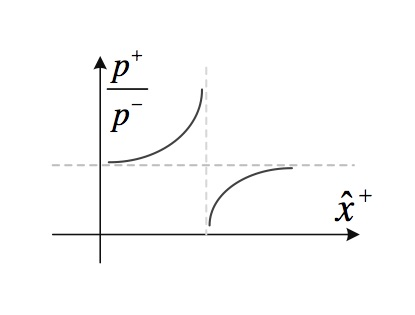
\includegraphics[scale=0.6]{gap.jpeg}
	\caption{有偏对比损失与互信息优化示意图}
	\label{Fig:gap}
\end{figure}
图~\ref{Fig:gap}展示了公式~\eqref{eq:fractional}作为分数函数的近似形状,揭示了使用PU数据时,InfoNCE $\mathcal{L}_\textsc{Biased}$损失优化和互信息(MI)优化之间的不一致性。也就是说,在使用PU数据优化InfoNCE损失时,增加$\hat{x}^+$并不会导致保存互信息的密度比$p^+/p^-$的单调增加。跳跃间断点的存在表明,$\mathcal{L}_\textsc{Biased}$的优化不一定会导致可控的MI优化。MI优化的难题源于以下事实:并非所有的$\{x_i^\prime\}_{i=1}^N$都是$\textsc{Tn}$样本,因为它们是从数据分布$ p_d $中随机抽取的。这导致在分解数据分布$ p_d $时,公式~\eqref{eq:gap}的分母中包含了$ p^+$。图~\ref{Fig:illustrative}提供了直观的解释。这五个随机抽样的样本实际上包含一个伪负例$\textsc{Fn}$样本。这样的伪负样本应该被拉近到锚点$x$附近。然而,由于它被错误地当作负样本,在模型训练过程中它将被推离锚点,从而破坏了嵌入表示的语义结构~\cite{Feng:2021:CVPR}。



\section{贝叶斯自监督对比损失函数设计}
\subsection{对齐性与均匀性困境}\label{subsec:fh}

首先介绍伪负例和困难负例的概念。在个性化推荐任务中,对于某个用户,伪负例(False Negative Sample)是用户没看见但潜在喜欢的物品;困难负例(Fard Negative Sample)是用户不喜欢但是很容易被误判为喜欢的物品,与用户喜欢的物品相似,常见于流行度较高的热门物品。由于偏好的概念并不直观,图\ref{Fig:illustrative}借用图像分类任务例子,提供了伪负例和困难负例的一个更直观的解释。对于一个锚点为“狗”的图像,正例通过语义不变的图像增强获得,负例从未标记样本中随机抽样,假设共得到五个未标记样本$\{x_1^\prime,x_2^\prime,x_3^\prime,x_4^\prime,x_5^\prime\}$。其中$x_3^\prime$的真实标签是“狗”,是与锚点同类的伪负例(FN)。剩余4个随机负样本是与锚点不同类的真负例(TN),其中$x_1^\prime$的真实标签与锚点不同类的“狼”,但是它与正例“狗”这个类很相似,视觉上难以区分,是困难负例。

%这个例子也可以类比在推荐系统中,略微的差异是锚点的选择,图像中任意样本都可以做锚点,而在推荐系统中通常只有用户才会作为锚点。推荐系统中的正例是从观测到的交互中获得,负例是从未交互的物品中随机抽样获得。根据未标注样本标签的不同,同样也面临着上述硬负例挖掘和伪负例去偏的任务。
%*******************************
\begin{figure*}[!]
	\centering
	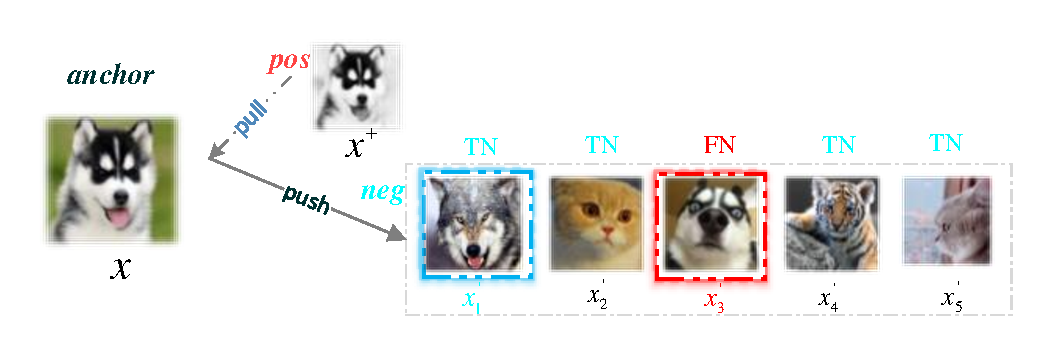
\includegraphics[width=0.9\textwidth]{pucon.pdf}
	\caption{自监督对比学习的伪负例去偏和硬负例挖掘示意图}
	\label{Fig:illustrative}
\end{figure*}
%*******************************

对比学习的任务是拉近正样本,推远负样本,一方面使得用户潜在喜欢的正例距离用户锚点较近,即出现在推荐列表排靠前的位置;另一方面,使得用户不喜欢的负例距离用户锚点较远,即出现在推荐列表靠后的位置。由于随机负样本可能是真负例或者伪负例,那么根据未标注样本的标签不同,就存在两个不同的考量:
\begin{itemize}
\item \textit{伪负例去偏}:对于与锚点同类的伪负例$x_3^\prime$,应当防止它被推离锚点,保持“狗”这个类的样本距离比较近,也称为对齐(alignment)。在推荐系统中,这有助于实现用户喜欢的物品出现在排序列表靠前的位置。
\item \textit{硬负例挖掘}:对于与锚点不同类的真负例$x_1^\prime$,应当把它推远离锚点,保持“狗”和“狼”这两个类之间的样本距离比较远,也称为均匀(uniformity)。在推荐系统中,这有助于实现用户不喜欢的物品出现在排序列表靠后的位置。
\end{itemize}
对于一个未标注样本,由于不知道它的所属类别,因此不知道应该把它推远以实现均匀性,还是应该防止它被推远以实现对齐性。这一问题,被称为均匀性和对齐性困境\cite{zhang:cl,Feng:2021:CVPR}。

一个可行的方案是枚举未标注样本的真实标签的情况,然后进行极大似然估计。考虑$\{x_1^\prime,x_2^\prime,x_3^\prime,x_4^\prime,x_5^\prime\}$的标签,每个标签只有两种可能:用户喜欢时为真负例,用户不喜欢时为伪负例。根据二项式定理,五个未标注样本的真实标签共有$2^5=32$种可能的情况。当N很大时,枚举每一种情况,并对每一种情况进行极大似然估计是非常困难的,上一章的思想难以向较大负例个数N推广。

受到经典的重要性采样(Importance Sampling)技术的启发,可以在每个未标注样本$x_i^\prime$添加一个重要性权重$\omega_i$,从而灵活的实现样本的均匀性和对齐性,以解决对比损失在PU的隐式反馈数据集中优化目标偏离的问题。那么包含重要性权重的对比损失函数可以重写为
\begin{eqnarray}
	\small
	\mathcal{L} &=& \mathbb E_{ \substack{x \sim p_d\\~x^+ \sim p^+\\{~x^\prime \sim p_d}}}
	[-\log \frac{e^{f(x)^Tf(x^+)}}{e^{f(x)^Tf(x^+)} + \sum_{i=1}^{N} \omega_i \cdot e^{f(x)^Tf(x_i^\prime)}}] \nonumber \\
	&=& \mathbb E_{ \substack{x \sim p_d\\~x^+ \sim p^+\\{~x^\prime \sim p_d}}}
	[-\log \frac{\hat{x}^+}{{\hat{x}^+} + \sum_{i=1}^{N} \omega_i \cdot \hat{x}_i}] \label{eq:debias}
\end{eqnarray}
式~\eqref{eq:debias}是把正例与锚点的相似度得分$e^{f(x)^Tf(x^+)}$记为$\hat{x}^+$,把未标注样本与锚点的相似度得分$e^{f(x)^Tf(x^\prime)}$记为$\hat{x}$,以保持分析过程中符号的简洁性。
		
下面考察在包含重要性权重后,权重$\omega_i$是如何控制未标记样本$x^\prime_i$对模型的参数学习与更新。损失函数相对于模型的参数$\Theta$的梯度可以计算为:
\begin{eqnarray}
\frac{\partial\mathcal{L}}{\partial \Theta} &=& \frac{\partial\mathcal{L}}{\partial \hat{x}_i^\prime} \cdot \frac{\partial \hat{x}_i}{\partial\Theta} \\
&=&  \frac{ \omega_i\hat{x}_i} {\hat{x}^+ + \sum_{i=1}^{N} \omega_i \cdot \hat{x}_i}\cdot \frac{\partial \hat{x}_i}{\partial\Theta} \label{eq:rule}
\end{eqnarray}
式~\eqref{eq:rule}是微分的链式法则的结果,第一项$\frac{ \omega_i\hat{x}_i} {\hat{x}^+ + \sum_{i=1}^{N} \omega_i \cdot \hat{x}_i}$由损失函数的具体形式决定的,第二项$ \frac{\partial \hat{x}_i}{\partial\Theta}$由编码器和评分函数的形式决定的。可以看到,重要性权重$\omega_i$出现在第一项的分子,作用类似一个调节器,它直接控制了未标注样本$x_i^\prime$对模型参数更新的贡献大小,进而控制了这个未标注样本被推多远。

从正例对齐、负例均匀的任务目标考虑,合意的权重$\omega_i$应该满足如下要求:
\begin{itemize}
\item 如果未标注样本$x_i^\prime$是一个和锚点同类的伪负例,合意的权重$\omega_i$应该取值较小,最好是0,以防止正样本被推远,使得同类样本距离较近,体现\textit{伪负例去偏原则}。伪负例可以看作负样本中出现的噪声,较小的$\omega_i$可以使得式~\eqref{eq:rule}的梯度消失,能够防止模型学到噪声样本的模式,避免推荐模型误判用户的兴趣边界。
\item 如果未标注样本$x_i^\prime$是一个和锚点不同类的真负例,合意的权重$\omega_i$应该取值较大,以推远硬负样本,使得不同类样本距离较远,体现\textit{硬负例挖掘原则}。困难负样本可以看作难以拟合的负样本,较大的$\omega_i$可以使得式~\eqref{eq:rule}的梯度幅度增加,激励模型去学习难以区分的样本,从而学习更加准确的用户兴趣边界。
\end{itemize}

综合上面的分析,合意的$\omega_i$与相应的未标注样本$x^\prime_i$的所属类别相联系:\textit{未标注样本$x^\prime_i$是真负例的概率越低,权重$\omega_i$值应该越小(伪负例去偏要求);未标注样本$x^\prime_i$是真负例的概率越高,权重$\omega_i$应该越大(硬负例挖掘要求)}。下面章节将介绍如何计算一个合意的重要性权重,满足上述要求。

\subsection{重要性权重计算}
\subsubsection{相似度分数分布}
根据重要性采样的规定步骤,需要目标抽样群体的硬负例的分布,和实际抽样群体的未标注样本的分布,那么重要权重为目标抽样群体和实际抽样群体分布的密度比。为了得到这个权重,首先聚焦于未标注样本与锚点的相似度分数$\hat{x}$,它更一般的形式化表示方式为$\exp(\text{sim}(f(x),f(x^\prime))/t)$,其中$f(\cdot)$是基于深度神经网络的编码器编码的表示向量,$\text{sim}(f(x),f(x^\prime))$表示锚点嵌入和未标记样本嵌入的相似度,如内积余弦相似度等。$t$为温度系数。

视未标注样本$x^\prime$为随机变量,则相似度分数$\hat{x} = \exp(\text{sim}(f(x),f(x^\prime))/t)$的分布的影响因素众多:与锚点$x$的选择有关,与神经网络$f(\cdot)$的结构有关,也与相似度函数$\text{sim}(\cdot,\cdot)$的具体形式有关。第\ref{cha:2}章的引理~\ref{Lemma2:AprioriDistribution}讨论了,在取似度函数$\text{sim}(\cdot,\cdot)$为向量内积时,即使是简单的两个高斯随机向量的相似度,其分布表达式也是非常复杂的,经过非线性函数$\exp(\cdot/t)$映射以后,想获取其密度表达式更加困难。因此,第\ref{cha:2}章的方法,以及现有的研究\cite{Xia:2022:ICML}通过高斯混合模型\cite{Lindsay:1995}、Beta混合模型~\cite{Xia:2022:ICML}等参数化方法来拟合未标注样本的相似度分数$\hat{x}$分布,引入了过强的假设,不具一般性。此外,用于密度估计的学习算法是昂贵的,因为混合系数是隐藏变量,只能通过EM算法~\cite{Dempster:1977:RSS}的迭代数值计算来获得,且算法对初始值非常敏感。

本节提出了一种方法,无需显式地估计相似度分数分布,即可实现对密度比的解析计算。对于固定的锚点,假设该锚点与其他未标注样本的相似度分数$\hat{x}$独立同分布于某个锚点特定的未知分布$\phi$,即
\begin{eqnarray}
\hat{x} \sim \phi(\hat{x})
\end{eqnarray}
相应的累积分布函数$\Phi(\hat{x})=\int_{-\infty}^{\hat{x}} \phi(t) dt$。注意,分布$\phi$是特定于锚点的,不同锚点对应的相似度分数分布不必相同。由于不对分布$\phi$做出任何假设,因此本方法属于非参数方法。根据上述抽象表达式,结合第\ref{cha:intro1}章介绍的次序统计量知识,可以写出它对应的次序统计量分布为:
\begin{align}
	\phi_{(1)}(\hat{x}) &= 2\phi(\hat{x}) [1-\Phi(\hat{x})] \label{eq:order1} \\
	\phi_{(2)}(\hat{x}) &= 2\phi(\hat{x}) \Phi(\hat{x}) \label{eq:order2}
\end{align}

\subsubsection{目标采样群体}
对于固定的锚点,若未标注样本是伪负例,则记该未标注样本与锚点的相似度分数$\hat{x} \in \textsc{Fn}$,表明这是一个来自伪负例的相似度分数,所有的伪负例相似度分数总体对应的类条件概率密度记为$\phi_\textsc{Fn}$。类似地,若随机样本是真负例,则记该未标注样本与锚点的相似度分数$\hat{x} \in \textsc{Tn}$,表明这是一个来自伪负例的相似度预测分数,所有的真负例相似度分数总体的类条件概率密度记为$\phi_\textsc{Fn}$。

接下来,可以通过正样本和负样本的表示在超球面上的相对位置,解析真负例的类条件概率密度$\phi_{\textsc{Tn}}$表达式。考虑一个锚点、正例和真负例构成的$(x, x^+, x^-)$三元组,其得分预测有且只有两种可能的情况:(a) 负例得分预测小一些,即 $ \hat{x}^- < \hat{x}^+ $, (b) 负例得分预测大一些,即 $ \hat{x}^+ \leq \hat{x}^- $。


%存在一个以$ f(x) $为中心、半径为$ d^+ $的闭球$ \mathfrak{B}[f(x),d^+] =\{f(\cdot)| d(f(x),f(\cdot)) \leq d^+ \}$,其中$ d^+ = \|f(x)-f(x^+)\|$是锚点嵌入$ f(x) $和正样本嵌入$ f(x^+) $之间的距离。那么,真负例的相对位置有且只有两种可能情况:$ f(x^-) \in \mathfrak{B}[f(x),d^+] $或$ f(x^-) \notin \mathfrak{B}[f(x),d^+] $。

\begin{figure}[!]
	\centering
	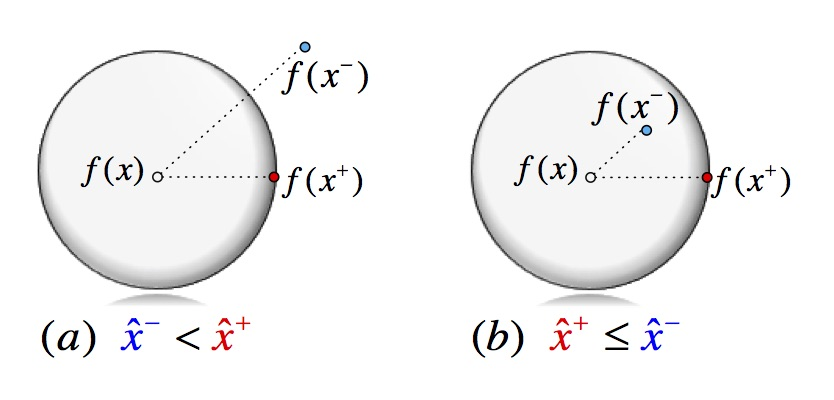
\includegraphics[scale=0.35]{openball.jpeg}
	\caption{正负样本对相对位置示意图}
	\label{Fig:openball}
\end{figure}

图~\ref{Fig:openball}描述了这两种可能的情况:图~\ref{Fig:openball}(a)情况对应正例与锚点距离更近,即$ d^+ < d^- $;图~\ref{Fig:openball}(b)情况对应于负例与锚点距离更近,即$ d^- \leq d^+ $,其中$ d^{-}=\|f(x) - f(x^-)\|$是欧式距离度量。对于情况(a),必有$ \hat{x}^- < \hat{x}^+ $,对于情况(b),必有$ \hat{x}^+ \leq \hat{x}^- $。这是因为所有嵌入$ f(\cdot) $都在半径为$ 1/t $的超球面上,那么欧氏距离与相似度分数一一对应,存在如下关系:$ d^\pm = \sqrt{2/t^2 - 2f(x)^\mathsf{T} f(x^\pm)}$。

对于关心的真负例相似度分数$ \hat{x}^- $,在图~\ref{Fig:openball}中用蓝色进行了标记,在情况(a)下,它是次序统计量$ X_{(1)} $的一个取值,在情况(b)下是次序统计量$ X_{(2)} $的一个取值。记情况(a)发生的概率为$\alpha$,情况(b)发生的概率为$1-\alpha$。那么,真负例的相似度分数观测值的生成过程可以描述如下:以概率$\alpha$选择情况(a),然后从次序统计量分布$\phi_{(1)}$生成观测值$\hat{x}$;或者以概率$1-\alpha$选择情况(b),然后从次序统计量分布$\phi_{(2)}$生成观测值$\hat{x}$。也就是说,真负例的类条件概率密度是$\phi_{\textsc{Tn}}$是成分$\phi_{(1)}$和成分$\phi_{(2)}$以系数$\alpha$进行混合构成:
\begin{eqnarray}
	\phi_{\textsc{Tn}}(\hat{x}) = \alpha \phi_{(1)}(\hat{x}) + (1-\alpha)\phi_{(2)}(\hat{x}) \label{eq:phitn}
\end{eqnarray}

类似地,伪负例相似度分数的类条件概率密度$\phi_{\textsc{Fn}}$是成分$\phi_{(2)}$和成分$\phi_{(1)}$以系数$\alpha$进行混合构成:
\begin{eqnarray}
	\phi_{\textsc{Fn}}(\hat{x}) = \alpha \phi_{(2)}(\hat{x}) + (1-\alpha)\phi_{(1)}(\hat{x})\label{eq:phifn}
\end{eqnarray}

需要说明的是,次序统计量$X_{(1)}$的定义是满足$X_{(1)}\leq X_{(2)}$。在情况(a)下$\hat{x}^- < \hat{x}^+$,将真负例的相似度分数$\hat{x}^-$视作次序统计量$X_{(1)}$的一个取值,忽略了$\hat{x}^- = \hat{x}^+$的特殊情况。对于这种特殊情况$\hat{x}^-$的概率测度为0,因为$\phi$是由Lebesgue测度控制的连续密度函数。直观地理解,对于任意连续概率密度函数如高斯分布,随机变量取任意离散点的概率为0。下面的引理证明了,类条件概率密度$\phi_{\textsc{Tn}}$和$\phi_{\textsc{Fn}}$满足概率密度函数的非负性和归一性要求。

\begin{lemma}[类条件概率密度]
若相似度分数的分布$\phi(\hat x)$是连续的概率密度函数,满足正定性$\phi(\hat x) \geq 0 $和归一性$\int_{-\infty}^{+\infty}\phi(\hat x) d\hat x =1 $,那么

(1) $\phi_{\textsc{Tn}}(\hat{x})$是概率密度函数,满足$\phi_{\textsc{Tn}}(\hat{x})\geq 0$,且$\int_{-\infty}^{+\infty}\phi_{\textsc{Tn}}(\hat{x})d\hat x =1 $。

(2) $\phi_{\textsc{Fn}}(\hat{x})$是概率密度函数,满足 $\phi_{\textsc{Fn}}(\hat{x})\geq 0$,且  $\int_{-\infty}^{+\infty}\phi_{\textsc{Fn}}(\hat{x})d\hat x =1 $。
\begin{proof}
由于 $\phi(\hat x) \geq 0 $ 且 $\int_{-\infty}^{+\infty}\phi(\hat x) d\hat x =1 $, 因此
	\begin{eqnarray}
		\phi_{\textsc{Tn}}(\hat{x}) &=& \alpha \phi_{(1)}(\hat{x}) + (1-\alpha)\phi_{(2)}(\hat{x}) \nonumber \\ 
		&=& 2\alpha\phi(\hat{x}) [1-\Phi(\hat{x})]+ 2(1-\alpha)\phi(\hat{x}) \Phi(\hat{x}) \nonumber \\ 
		&\geq& 0,
	\end{eqnarray}
其中 $\Phi(\hat{x}) \in [0,1]$. 
	\begin{eqnarray}
		\int_{-\infty}^{+\infty}\phi_{\textsc{Tn}}(\hat{x})d\hat x &=& \int_{-\infty}^{+\infty}2\alpha\phi(\hat{x}) [1-\Phi(\hat{x})]+ 2(1-\alpha)\phi(\hat{x}) \Phi(\hat{x}) d\hat x \nonumber \\
		&=&2\alpha\int_{-\infty}^{+\infty}\phi(\hat{x}) [1-\Phi(\hat{x})] d\hat x+  2(1-\alpha)\int_{-\infty}^{+\infty} \phi(\hat{x}) \Phi(\hat{x}) d\hat x \nonumber \\
		&=&2\alpha\int_{-\infty}^{+\infty} [1-\Phi(\hat{x})] d\Phi(\hat{x}) +  2(1-\alpha)\int_{-\infty}^{+\infty}  \Phi(\hat{x}) d\Phi(\hat{x}) \nonumber \\
		&=& 2\alpha\int_{0}^{1} (1-\mu) d\mu +  2(1-\alpha)\int_{0}^{1}  \mu d\mu  \label{Eq:sub}\\
		&=& [\alpha(2\mu-\mu^2) +(1-\alpha)\mu^2] \big|_0^1 \nonumber \\
		&=&1,
	\end{eqnarray}
其中,公式~\ref{Eq:sub}是对$\Phi(\hat{x})$和$\mu$进行换元积分。同样地,
	\begin{eqnarray}
		\phi_{\textsc{Fn}}(\hat{x}) &=& \alpha \phi_{(2)}(\hat{x}) + (1-\alpha)\phi_{(1)}(\hat{x}) \nonumber\\
		&=& 2\alpha \phi(\hat{x}) \Phi(\hat{x}) +2(1-\alpha)\phi(\hat{x}) [1-\Phi(\hat{x})] \nonumber \\ 
		&\geq& 0,
	\end{eqnarray}
且
	\begin{eqnarray}
		\int_{-\infty}^{+\infty}\phi_{\textsc{Fn}}(\hat{x})d\hat x &=& 2\alpha\int_{-\infty}^{+\infty}  \phi(\hat{x}) \Phi(\hat{x})d\hat x +2(1-\alpha)\int_{-\infty}^{+\infty}\phi(\hat{x}) [1-\Phi(\hat{x})] d\hat x \nonumber \\
		&=& 2\alpha\int_{-\infty}^{+\infty} \Phi(\hat{x})d\Phi(\hat{x}) +2(1-\alpha)\int_{-\infty}^{+\infty}[1-\Phi(\hat{x})] d\Phi(\hat{x}) \nonumber \\
		&=& 2\alpha\int_{0}^{1}  \mu d\mu +2(1-\alpha)\int_{0}^{1} (1-\mu) d\mu \nonumber \\
		&=& [\alpha \mu^2 + (1-\alpha) (2\mu - \mu^2) ]\big|_0^1 \nonumber \\
		&=&1.
	\end{eqnarray}
证毕。
\end{proof}
\end{lemma}

通过查看图~\ref{Fig:openball},有助于进一步理解混合系数$\alpha$的含义:$\alpha$描述了情况(a)发生的概率,即编码器将伪负例(正例)编码到比负例更近的距离的概率,也即正例评分高于负例评分的概率。对于一个随机盲猜的最差编码器$ f $,$\alpha=0.5$;而对于一个完美的编码器$\alpha=1$。因此,合理的$\alpha$值应在$[0.5, 1]$范围内。实际上,$\alpha$的含义就是当前训练时点的编码器的AUC,它对应于数据集$\mathcal{D}$中所有锚点$ x $宏平均的AUC经验估计:
%*******************************
\begin{figure}[!]
	\centering
	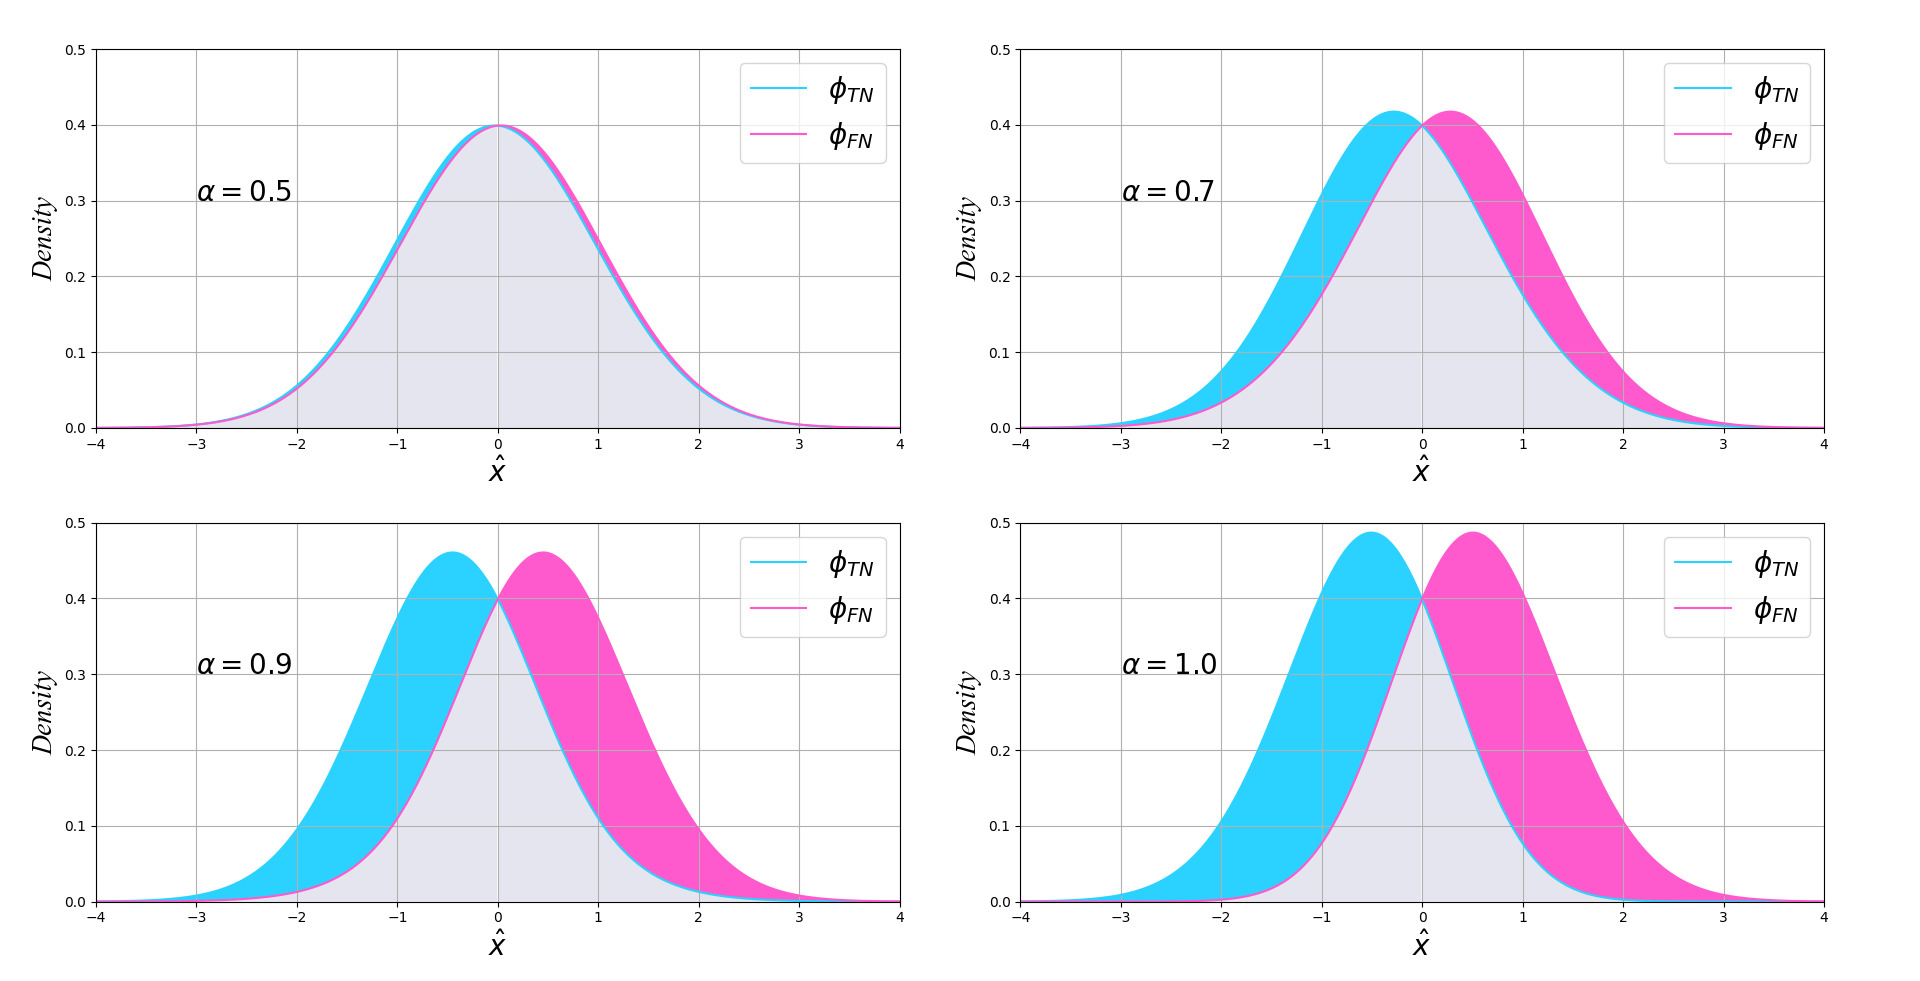
\includegraphics[width=\textwidth]{theorydist.png}
	\caption{不同$\alpha$设定下类条件概率密度示意图}
	\label{Fig:theorydist}
\end{figure}
%*******************************
\begin{eqnarray}
	\small
	\alpha &=& \int\limits_{x \in \mathcal{X}}  \int\limits_{0}^{+\infty} \int\limits_{0}^{+\infty} \mathbb I (\hat{x}^+ \ge \hat{x}^-)  p(\hat{x}^+ , \hat{x}^-) p(x) d\hat{x}^+  d\hat{x}^- dx\nonumber\\
	&\simeq& \frac{1}{|\mathcal{D}|} \frac{1}{|\mathcal{D}^+| |\mathcal{D}^-|} \sum_{\mathcal{D}^+}\sum_{\mathcal{D}^-}  \mathbb I (\hat{x}^+ \ge \hat{x}^-) \nonumber \\
	&=& \frac{1}{|\mathcal{D}|} AUC
\end{eqnarray}
因此$\alpha$的值可以通过少部分标记的样本进行经验估计,或者作为超参数。因此,本章不再局限于第\ref{cha:thirdsection}章负采样算法所提出的“负例分数小于正例”的序关系假设。

通过将公式~\eqref{eq:order1}和公式~\eqref{eq:order2}中的似度分数分布$\phi(\hat{x})$设定为$\mathcal{N}(0,1)$,可以作为一个实例,帮助了解$\alpha$如何影响公式~\eqref{eq:phitn}和公式~\eqref{eq:phifn}中的类条件概率密度$\phi_{\textsc{Tn}}(\hat{x})$和$\phi_{\textsc{Fn}}(\hat{x})$,如图~\ref{Fig:theorydist}所示。较大的$\alpha$值导致$\phi_{\textsc{Tn}}(\hat{x})$与$\phi_{\textsc{Fn}}(\hat{x})$之间的区分度更高,因为更好的编码器会将具有不同类标签的样本编码得更正交~\cite{Chuang:2020:NIPS}。需要说明的是,将布$\phi(\hat{x})$设定为$\mathcal{N}(0,1)$只是为了解释说明,后续计算不涉及任何对$\phi(\hat{x})$的具体形态的假设。

真负例分数的类条件概率密度$\phi_{\textsc{Tn}}(\hat{x})$,就是理想的\textit{目标抽样群体},描述了来自真负样本群体的相似度分数分布。使用来自这部分的样本计算得到的损失函数,即为有监督损失。它由两个成分组成:抵押给组成成分是~\ref{Fig:illustrative}中$x_1^\prime$(狼)这个困难负样本的相似度分数,它是与锚点类别不同的负样本,但是由于和锚点很相似,导致它被投影到了一个距离锚点更近的距离,这种情况对应于图\ref{Fig:openball}(b)中所描述的情况,即真负例距离锚点更近,属于被错分的样本。这类硬负例的相似度分数密度对应于式\eqref{eq:phitn}中的第二项,即$(1-\alpha)\phi_{(2)}(\hat{x})$,称为\textit{困难负样本成分};另外一类容易负样本如\ref{Fig:illustrative}中$x_5^\prime$(猫),它容易区分,被投影到了一个距离锚点更远的距离,对应于图\ref{Fig:openball}(a)中所描述的情况,这类容易负样本的相似度分数密度对应于式\eqref{eq:phitn}中的第一项,即$\alpha\phi_{(1)}(\hat{x})$,称为\textit{容易负样本成分}。

困难负样本由于与锚点非常相似,难以区分,总是被编码到锚点比较近的距离,不利于下游分类任务。为了加大对真负例总体$\phi_{\textsc{Tn}}(\hat{x})$中困难负样本成分$(1-\alpha)\phi_{(2)}(\hat{x})$的采用力度,引入一个参数$\beta \in [0.5, 1]$,对真负例的群体$\phi_{\textsc{Tn}}(\hat{x}) $进行细分,从困难负样本成分中抽样$\beta$的比例,从容易负样本成分中抽样$1-\beta$的比例,构成新的抽样目标:
\begin{eqnarray}
	\phi_{\textsc{Thn}}(\hat{x}) 
	&=& (1-\beta)\alpha  \phi_{(1)}(\hat{x}) +\beta (1-\alpha)  \phi_{(2)}(\hat{x}) \label{eq:tnhard} 
\end{eqnarray}
参数$1-\beta$控制着\textit{易负样本成分}$\alpha \phi_{(1)}(\hat{x})$的比例,而$\beta$控制着被分类器错误分类的\textit{困难负样本成分}$(1-\alpha)\phi_{(2)}(\hat{x})$的比例。$\beta= 1$时,新的目标抽样群体$\phi_{\textsc{Thn}}(\hat{x}) $只有困难负样本成分;$\beta = 0.5$时,容易负样本成分和困难负样本的比例与原始抽样目标是一致的;$\beta = 0$时,新的目标抽样群体$\phi_{\textsc{Thn}}(\hat{x}) $只有容易负样本成分;因此,公式~\eqref{eq:tnhard}可以解释为具有困难级别(Hardness Level)为$\beta$的困难负样本分布,较大的$\beta$值(接近1)导致目标抽样群体中包含更高比例的被分类器错误分类的困难负样本成分。

\subsubsection{实际采样群体}
实际采样的样本来自未标注样本,通过正样本和负样本的类条件密度,可以应用全概率公式将边缘概率与条件概率联系起来,从而获得未标记数据的密度$\phi_{\textsc{Un}}$
\begin{eqnarray}\label{eq:unlabel}
	\phi_{\textsc{Un}} &=& \tau^-\phi_{\textsc{Tn}} +\tau^+\phi_{\textsc{Fn}}  
\end{eqnarray} 
未标注样本的概率密度决定性因素是伪负例的类先验概率$\tau$。一个伪负例占比为50\%的数据集,和伪负例占比为5\%的数据集,相似度的分数分布差别是很大的。

为了避免混淆,表\ref{table:density}梳理了本章出现的密度的符号及含义。需要特别强调的是相似度分数分布$\phi(\hat{x})$与未标记样本的相似度分数分布$\phi_{\textsc{Un}}(\hat{x})$的区别:前者由锚点$x$,相似度函数,以及编码器结构$f$决定,包含了所有的可能的类先验$\tau$可能的取值的分布;而后者未标记样本的相似度分数分布$\phi_{\textsc{Un}}(\hat{x})$由特定的类先验$\tau$决定。
\begin{table*}[h!]
	\centering
	\caption{概率密度一览表}\label{table:density}
	\resizebox{1\textwidth}{!}{
		\begin{tabular}{cllc}
			\toprule[1.2pt]	
			\textbf{符号}&\textbf{含义}& \textbf{描述}&是否包含参数化假设 \\ \hline		
			$\phi(\hat{x})$ & 特定于锚点的相似度分数分布 & 由锚点$x$,相似度函数,以及编码器结构$f$决定 & 否 \\
			$\phi_{(1)}(\hat{x})$ &次序统计量$X_{(1)}$的分布& 由$\phi(\hat{x})$决定& 否\\
			$\phi_{(2)}(\hat{x})$ &次序统计量$X_{(2)}$的分布& 由$\phi(\hat{x})$决定 & 否 \\\hline
			$\phi_{\textsc{Tn}}(\hat{x})$&真负例相似度分数的类条件概率密度& \textbf{目标抽样群体} & 否 \\
			$\phi_{\textsc{Fn}}(\hat{x})$&伪负例相似度分数的类条件概率密度& -- & 否 \\
			$\phi_\textsc{Thn}(\hat{x})$& 硬负例的相似度分数分布&通过细分$\phi_{\textsc{Tn}}(\hat{x})$得到的\textbf{新的目标抽样群体}& 否  \\\hline
			$\phi_{\textsc{Un}}(\hat{x})$& 未标记样本的相似度分数分布&\textbf{实际抽样群体}& 否  \\
			\hline
			\bottomrule[1.2pt]
			
			~		\end{tabular}
	}
\end{table*}


\subsubsection{蒙特卡洛重要性采样}
上面的分析只得到了目标抽样群体和实际抽样群体密度函数的抽象表达式,足以解析地计算重要性权重$\omega_i$。根据经典的蒙特卡洛重要性采样~\cite{Hesterberg:1988,Bengio:2008:TNN}的计算步骤,重要性权重的计算公式为目标抽样群体与实际抽样群体的密度比
%\begin{eqnarray}
%	\mathbb E_{\hat{x} \sim \psi}  \hat x 	&=& \int_{+\infty}^{+\infty} \hat x  \frac{\phi_\textsc{Thn}(\hat{x};\alpha, \beta)}{\phi_{\textsc{Un}}(\hat{x})} \phi_{\textsc{Un}}(\hat{x}) d\hat{x} \nonumber \\
%	&=&   \mathbb E_{\hat{x} \sim \phi_{\textsc{Un}}} \hat x  \frac{\phi_\textsc{Thn}(\hat{x};\alpha, \beta)}{\phi_{\textsc{Un}}(\hat{x})} \nonumber\\
%	&\simeq&\frac{1}{N}  \sum_{i=1}^{N} \omega_i \hat{x}_i  \label{eq:impor}
%\end{eqnarray}
\begin{eqnarray}
	\omega_i(\hat x_i;\alpha, \beta)&=& \frac{\phi_\textsc{Thn}(\hat{x};\alpha, \beta)/Z}{\phi_{\textsc{Un}}(\hat{x})} \label{eq:ome} \\
	&=& \frac{1}{Z} \frac{(1-\beta)\alpha + (\beta-\alpha)\Phi(\hat{x})}{\alpha\tau^- + (1- \alpha)\tau^+  + (1-2\alpha)\Phi(\hat{x})(\tau^- -\tau^+)}  \label{eq:ome1}
\end{eqnarray}
其中Z为目标抽样分布$\phi_\textsc{Thn}$的归一化配分因子,可以通过边缘积分准确计算如下:
\begin{eqnarray}
	Z &=& \int_{ - \infty } ^{\infty} \phi_{\textsc{Thn}}(\hat{x})  d \hat{x} \nonumber \\
	&=& \int_{-\infty}^{\infty}  [(1-\beta)\alpha  \phi_{(1)}(\hat{x}) +\beta (1-\alpha)  \phi_{(2)}(\hat{x})]  d \hat{x} \nonumber \\
	&=& (1-\beta)\alpha + \beta (1-\alpha)
\end{eqnarray}

可以看到式\eqref{eq:ome1}中的重要性权重$\omega_i(\hat x_i;\alpha, \beta)$是累积分布函数(CDF)$\Phi (\hat{x})$的函数, 而概率密度函数$\phi{(\hat{x})}$由于式\eqref{eq:ome1}的分式形式,可以通过约分被消去,进而无需对密度函数的具体形式做出任何参数化假设。只需要累计分布函数(C.D.F)
$\Phi (\hat{x})$的值,就可以计算相应的重要性权重。

下面介绍如何计算累积分布函数(C.D.F)$\Phi (\hat{x})$。
%\begin{eqnarray}
%	\phi_{\textsc{Un}}(\hat{x}) &=& \tau^-\phi_{\textsc{Tn}}(\hat{x}) +\tau^+\phi_{\textsc{Fn}}(\hat{x}) \nonumber \\
%	&=& 2\phi(\hat{x})[\alpha\tau^- + (1- \alpha)\tau^+  + (1-2\alpha)\Phi(\hat{x})(\tau^- -\tau^+)] \label{eq:unlabel1}
%\end{eqnarray}
对公式\eqref{eq:unlabel}等号两侧进行积分,可得:
\begin{eqnarray}
\int_{-\infty}^{\hat x}  \phi_{\textsc{Un}}(t) dt 
	&=& \int_{-\infty}^{\hat x} \tau^-\phi_{\textsc{Tn}}(t) +\tau^+\phi_{\textsc{Fn}}(t) dt \label{eq:un}\\
	&=& \int_{-\infty}^{\hat x} 2\phi(t)[\alpha\tau^- + (1- \alpha)\tau^+  + (1-2\alpha)\Phi(t)(\tau^- -\tau^+)] dt\nonumber\\ 
	&=&  2[\alpha\tau^- + (1- \alpha)\tau^+]\int_{-\infty}^{\hat x} \phi(t) dt + (1-2\alpha)(\tau^- -\tau^+)\int_{-\infty}^{\hat x} 2 \phi(t) \Phi(t) dt \nonumber\\
	&=& 2[\alpha\tau^- + (1- \alpha)\tau^+] \Phi(\hat{x}) + (1-2\alpha)(\tau^- -\tau^+)\Phi^2(\hat{x}) \label{eq:unlabel33}
\end{eqnarray}
式\eqref{eq:un}等号左侧对密度函数积分,正是累积分布函数$\Phi_{\textsc{Un}}(\hat{x})$。记
\begin{eqnarray}
	a &=&  (1-2\alpha)(\tau^- -\tau^+)\nonumber \\
	b &=& 2[\alpha\tau^- + (1- \alpha)\tau^+] \nonumber
\end{eqnarray}
那么式\eqref{eq:unlabel33}可以简化为一个一元二次方程
\[\Phi_{\textsc{Un}}(\hat{x})= a\Phi^2(\hat{x}) + b\Phi(\hat{x})\]
根据求根公式有
\begin{eqnarray}\label{eq:Phi}
	\Phi(\hat{x}) = \frac{-b+\sqrt{b^2+4a\Phi_{\textsc{Un}}(\hat{x})}}{2a}
\end{eqnarray}
另外一个解$\Phi(\hat{x}) = \frac{-b-\sqrt{b^2+4a\Phi_{\textsc{Un}}(\hat{x})}}{2a}$ 小于0舍去,因为它不在累积分布函数的取值区间内。上式建立了两个累积分布函数之间的关系,只要给出未标注样本的累积分布函数$\Phi_{\textsc{Un}}(\hat{x})$,就可以计算得到所需的$\Phi(\hat{x})$,从而用于计算重要性权重。
%%*******************************Fig~\ref{fig:cdf_trans} illustrates the transformation of two cumulative distribution functions $\Phi(\hat{x})$ and $\Phi_{\textsc{Un}}(\hat{x})$, where we fixed $\tau^+=0.1$. 
%\begin{figure*}[h!]
%	\centering
%	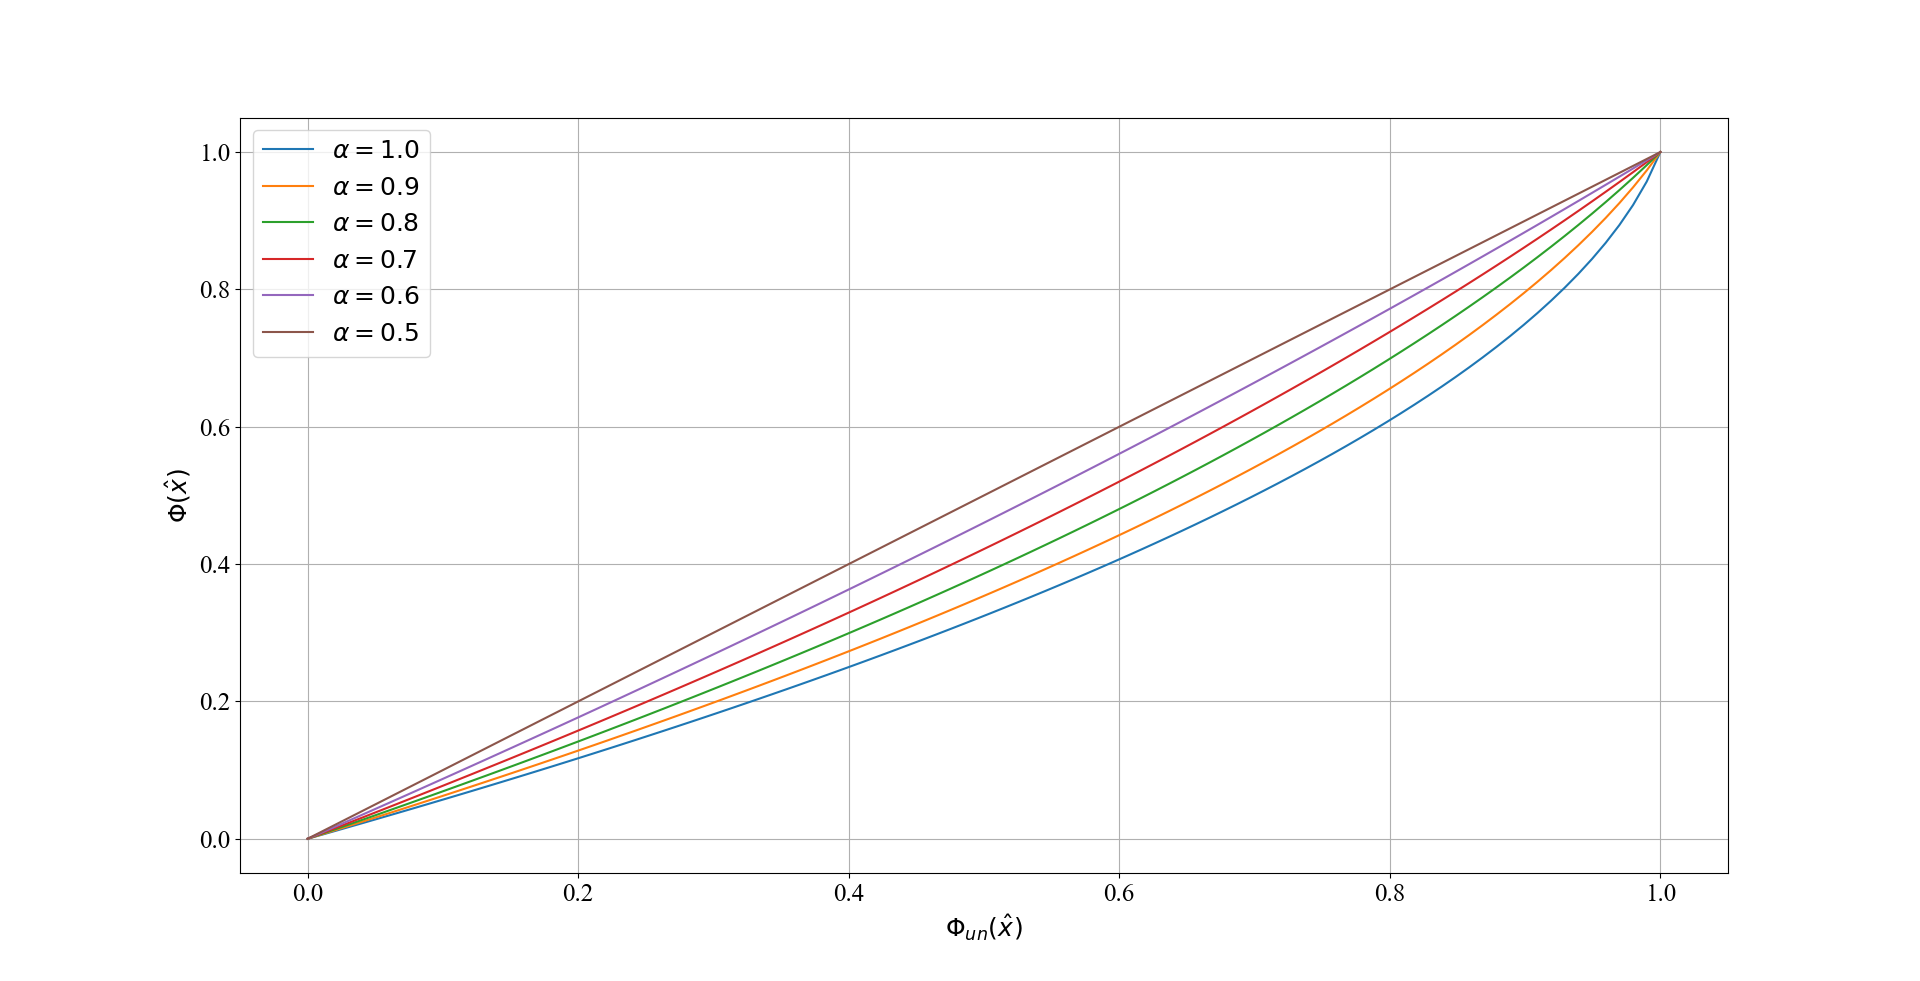
\includegraphics[width=\textwidth]{cdf_trans.png}
%	\caption{The transformation of two cumulative distribution functions $\Phi(\hat{x})$ and $\Phi_{\textsc{Un}}(\hat{x})$, where x-axis is the  C.D.F of unlabeled samples $\hat{\Phi}_{\textsc{Un}}$ , and y-axis is the anchor specific C.D.F $\Phi(\hat{x})$. From Eq~\eqref{eq:unlabel1}, it can be seen that when $\alpha=0.5$, which means the encoder makes random guesses, or when $\tau^+=0.5$, which means the prior class probabilities of positive and negative examples are equal, $\Phi(\hat{x})=\Phi_{\textsc{Un}}(\hat{x})$.}
%	\label{fig:cdf_trans}
%\end{figure*}
%%*******************************

最后只剩下如何计算未标注样本的累积分布函数$\Phi_{\textsc{Un}}(\hat{x})$。可以使用如下经验分布函数进行近似:
\begin{equation}\label{eq:puedf}
	\hat \Phi_{\textsc{Un}} (\hat{x}) = \frac{1}{N} \sum_{i=1}^{N}\mathbb{I}_{|X_i \leq \hat{x}|},
\end{equation}
第\ref{cha:intro1}章第\ref{ecdf}小节提供了一个经验分布函数的计算实例。根据根据Glivenko定理~\cite{glivenko:1933}所述,经验累积分布函数$\hat{\Phi}_{\textsc{Un}}(\hat{x})$收敛于标准的累积分布函数(C.D.F) $\Phi_{\textsc{Un}}(\hat{x}) = \int_{-\infty}^{\hat{x}} \phi_{\textsc{Un}}(t)dt$。

%通过使用宏$AUC$度量对编码器进行表征,引入可计算的经验累积分布函数作为似然度量来构建后验估计器,

到目前为止,重要性权重的计算已经介绍完毕。它们的计算只涉及以下内容:(1) $\hat{\Phi}_{\textsc{Un}} (\hat{x}) \in [0,1]$,它代表了贝叶斯视角下的\textit{样本信息},可以直接从N个未标注样本计算得出。它包含了当前模型对未标注样本是伪负例$\hat x \in \textsc{Fn}$的概率解释:对于较大的$\hat{x}$值(与锚点的嵌入距离更接近),$\hat{\Phi}_{\textsc{Un}} (\hat{x})$输出一个更接近于1的值,表明$\hat{x}$是一个来自伪负例的相似度观测值。换言之,$\hat{\Phi}_{\textsc{Un}} (\hat{x})$反映了当前模型对未标注样本的分类结果。(2)类别先验概率$\tau$。由样本信息和先验信息计算到的权重$\omega_i$自然包含后验信息,因此把经过上述重要性权重加权的自监督对比损失成为贝叶斯自监督对比损失(Bayesian self-supervised Contrastive Loss, BCL)。定理~\ref{the:poster}分析了权重$\omega$与样本是真负例的后验概率之间的联系,它们是严格的线性关系。


参数$\alpha\in [0.5,1]$对应于当前训练轮次下,编码器的宏AUC度量,控制着样本信息的置信水平。在训练过程中,可以通过验证数据集进行经验估计。参数$\beta\in [0.5,1]$对应于真负例群体中被错误分类的\textit{困难负样本成分}的比例,是一个根据任务场景所需的硬负例挖掘困难等级(Hardness Level)决定的超参数。在计算对比损失时,仍然是使用随机均匀采样的未标记样本$x_i^\prime$,但使用相应的重要性权重$\omega(\hat{x},\alpha, \beta)$进行加权,以校正目标采样群体和实际采样群体之间的偏差。那么,给定N个随机负采样的未标注样本$\{x_i^\prime\}_{i=1}^N$,校正后的损失函数形式为
\begin{eqnarray}\label{eq:bcl}
	\mathcal{L}_\textsc{~Bcl}=  \mathbb E_{\substack{x \sim p_d\\~x^+ \sim p^+\\\color{blue}{~x^\prime \sim p_d}}} [-\log \frac{e^{f(x)^Tf(x^+)}}{e^{f(x)^Tf(x^+)} +  \sum_{i=1}^N  \omega_i \cdot e^{f(x)^Tf(x^\prime_i)} }]
\end{eqnarray}

BCL和现有的工作HCL\cite{Robinson:2021:ICLR}都是通过重要性加权校正对比损失,但有以下不同:(1)从目标抽样群体来看,HCL假设未标记样本服从参数化的vMF分布,而BCL未假定任何参数化的分布;(2)从权重的计算方式来看,HCL的权重计算方式为$\omega_i^\textsc{Hcl} = \frac{g(\mathbf{x}^\prime_j)^\beta}{\frac{1}{N} \sum_{j=1}^{N}g(\mathbf{x}^\prime_j)^\beta}$,它是为标记样本相似度分数的函数,会因为用户物品嵌入的过度平滑(相似度分数趋同)导致权重消失。BCL的权重是经验分布函数$\Phi_{\textsc{Un}}(\hat{x})$的函数,它不受相似度分数趋同的影响,只受相对排序位置的影响;(3)从任务属性来看,HCL分配给相似度分数高的样本(困难样本)大权重,给相似度分数第的样本(容易样本)小权重,只考虑了硬负例挖掘任务;BCL根据样本是真负例的后验概率分配权重,给伪负例较小的权重,给硬负例较大的权重,兼顾了硬负例挖掘和伪负例去偏两个任务。

\section{算法实现与时间复杂度分析}
\subsection{算法步骤}
需要注意的是,蒙特卡洛重要性采样并不涉及显式地负采样。未标注样本仍然是基于随机样本,但额外地对随机样本进行重要性加权。重要性权重计算的逻辑有一些复杂,主要是解析目标采样分布和实际采样分布的抽象函数表达式,但计算步骤是很简单的,相对于标准的对比损失函数,只涉及三个额外计算步骤,如下伪代码所示。
\begin{algorithm}[!]
	\counterwithin{algorithm}{chapter}
	\SetKwInput{KwIn}{输入}  %<---细节与重点
	\SetKwInput{KwOut}{输出}  %<---细节与重点
	\SetAlgoLined
	\small
	\caption{贝叶斯自监督对比学习算法(BCL)伪代码}\label{5-Alg:1}
	\KwIn{数据条目组织形式为(锚点$x$,正例$x^+$,N个随机负采样的未标注样本$x_1^\prime, \cdots x_n^\prime$)的训练集$\mathcal{D}$,正例类先验$\tau^+$,去偏超参数$\alpha$, 硬负例难度超参数$\beta$。}
	\KwOut{模型参数$\Theta \in \mathbb{R}^d$。}
	~~计算正例分数$\hat{x}^+ = e^{f(x)^Tf(x^+)}$;\\
	计算N个未标注样本分数$\hat{x}_i = e^{f(x)^Tf(x^\prime_i)}$, $i = 1,2,\cdots, N$ ;
	
	\For{$i = 1,2,\cdots, N$}{
		~~通过公式\eqref{eq:puedf}计算经验分布函数$\hat \Phi_{\textsc{Un}} (\hat{x}_i)$; \\
		通过公式\eqref{eq:Phi}计算分布函数$\Phi(\hat{x}_i)$;\\
		通过公式\eqref{eq:ome1}计算重要性权重$\omega_i$;\\
		计算损失函数$\mathcal{L} = -\log \frac{\hat{x}^+}{\hat{x}^+ + \sum_{i=1}^N \omega_i \cdot \hat{x}_i}$;\\
		根据$\mathcal{L}$相对于$\Theta$的梯度更新参数$\Theta$;
	}
	\KwResult{模型参数$\Theta$。}
\end{algorithm}

将数据条目组织为(锚点$x$,正例$x^+$,N个随机负采样的未标注样本$x_1^\prime, \cdots x_n^\prime$)的元组结构,可以通过重写Pytorch的\verb|get_item|方法或\verb|collate_fn|方法实现,二者类似。第\ref{cha:fourthsection}章的算法\ref{4Alg2:1}提供了重写\verb|collate_fn|方法的算法伪代码,本章不再赘述。

\subsection{时间复杂度分析}
本章所介绍的方法,是上一章从$N=1$个负例向多个负例的更一般的对比损失的推广,但基本思想都是估计校正,不涉及显式的负采样,仍然使用随机负样本计算对比损失,因此也不涉及对mini-batch以外的额外计算和存储开销。由于BCL要计算重要性权重校正对比损失,从而引入了额外的时间复杂度。下面以标准的InfoNCE损失为基准,分析本章所提出的方法的计算的额外开销。

在计算标准的InfoNCE损失时,也需要正向计算正例的相似度分数以及未标注样本的相似度分数,然后反向传播按照梯度下降算法更新参数,那么InfoNCE也要执行算法\ref{5-Alg:1}最开始的两行。因此贝叶斯自监督对比学习的额外计算开销主要是:(1)通过公式\eqref{eq:puedf}计算经验分布函数$\hat \Phi_{\textsc{Un}} (\hat{x}_i)$,时间复杂度为$\mathcal{O}(N)$;(2)通过公式\eqref{eq:Phi}计算分布函数$\Phi(\hat{x}_i)$,时间复杂度为$\mathcal{O}(1)$;(3)通过公式\eqref{eq:ome1}计算重要性权重$\omega_i$,时间复杂度为$\mathcal{O}(1)$。计算重要性权重的公式\eqref{eq:ome1}尽管看起来很复杂,但是都是标量计算,因此是常数时间复杂度。因此,一个样本的重要性权重$\omega_i$额外计算开销为$\mathcal{O}(N)$。此时$N$为负例个数,而非物品总数,通常远低于编码样本$f(x)$的时间复杂度,是可以忽略的。在本章实验部分对比了实际的运行时间,本方法和基准方法InfoNCE相比,有着几乎相同的实际运行时间。

\section{贝叶斯自监督对比损失的理论分析}
本章的\ref{subsec:fh}小节分析了,基于对比学习“正例对齐、负例均匀”的任务考量,合意的权重$\omega_i$与相应的未标注样本$x^\prime_i$的所属类别相联系:未标注样本$x^\prime_i$是真负例的概率越低,权重$\omega_i$值应该越小(伪负例去偏要求);未标注样本$x^\prime_i$是真负例的概率越高,权重$\omega_i$应该越大(硬负例挖掘要求)。那么,本章的$\omega_i$值是否满足上述要求?本章计算的$\omega_i$与样本是真负例的概率有什么联系?此外,经过对随机样本的重要性加权以后计算得到的贝叶斯自监督对比损失,与完全监督数据计算得到的对比损失有什么联系?
%*******************************
\begin{figure}[!]
	\centering
	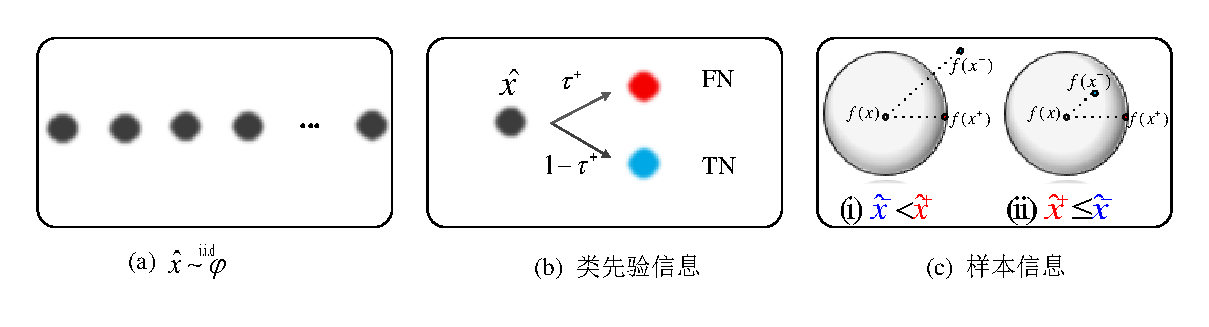
\includegraphics[width=\textwidth]{PCU.pdf}
	\caption{抽象数学模型示意图}
	\label{Fig:formulation}
\end{figure}
%*******************************
\subsection{小样本性质}
首先考察BCL损失计算的单个权重与样本是真负例的后验概率之间的联系。为了回答这个的问题,首先考虑一个如图\ref{Fig:formulation}描述的抽象数学模型:图\ref{Fig:formulation}(a)表示未标注样本$x^\prime_i$与锚点的相似度观测值$\hat{x}$为随机变量,假设它独立同分布于某个未知分布$\phi$,图\ref{Fig:formulation}(b)表示未标注样本观测值中,来自正类的占比为$\tau^+$,相应的观测值记为$\hat{x}^+$;未标注样本观测值中,来自负类的占比为$\tau^- = 1-\tau^+$,相应的观测值记为$\hat{x}^-$。图\ref{Fig:formulation}(c)表示正例的观测值以$\alpha$的概率小于负例的观测值。

图\ref{Fig:formulation}(a)是一个并不严格的假设,因为并没有对未知分布$\phi$的具体形态做出规定。对于不同的锚点,锚点与未标记样本的相似度分数观测值的分布$\phi$可以不同;图\ref{Fig:formulation}(b)不是假设,而是已知条件。正例类先验概率$\tau^+$通常是可以获得的,例如在类别均匀的10分类数据集中,遇到一个与锚点同类(狗)的同类样本的占比,就是1/10。更多面向复杂场景如类别不平衡、PU数据集的类先验$\tau^+$的估计方法可以参考文献\cite{Jain:2016:NIPS,Christoffel:2016:ACML};图\ref{Fig:formulation}(c)也不是假设,而是已知条件。前面的章节讨论了,$\alpha$的含义为当前模型参数下编码器的AUC,可以通过少部分标注样本进行经验估计,或者设定为超参数。

\begin{theorem}[后验概率估计]\label{the:poster}
设$\hat{x}$独立同分布于某未知分布$\phi$。其中,正例$\hat x^+$的占比为$\tau^+$,且$\mathbb P (\hat x^- < \hat x^+)= \alpha$ 。取$\beta = 0.5$,则重要性权重$\omega_i$与样本为真负例的后验概率$P(\textsc{Tn}|\hat{x}_i)$存在如下关系
\[\omega_i = \mathbb P(\textsc{Tn}|\hat{x}_i)/\tau^-\]
\begin{proof}
对于独立同分布于$\phi$的随机变量$\hat{x}$,其次序统计量$X_{(1)}$和$X_{(2)}$的分布为:
\begin{eqnarray}
	\phi_{(1)}(\hat{x}) &=& 2\phi(\hat{x}) [1-\Phi(\hat{x})] \nonumber \\
	\phi_{(2)}(\hat{x}) &=& 2\phi(\hat{x}) \Phi(\hat{x}) \nonumber
\end{eqnarray}
其中$\Phi(\hat{x}) = \int_{ - \infty }^{\hat{x}} \phi(t) dt$ 是概率密度函数$\phi(\hat{x})$对应的累积分布函数。

由于$\mathbb P (\hat x^- < \hat x^+)= \alpha$,则
\[\mathbb P (\hat x^- \geq \hat x^+)=1- \alpha\]

那么$\hat{x}$中的负例类别$\hat x^-$的概率密度是次序统计量$X_{(1)}$和$X_{(2)}$的概率密度以系数$\alpha$进行混合
\begin{eqnarray}
	\phi_{\textsc{Tn}}(\hat{x}) = \alpha \phi_{(1)}(\hat{x}) + (1-\alpha)\phi_{(2)}(\hat{x}) \nonumber
\end{eqnarray}
其中,负例类别$\hat x^-$的概率密度,也称类条件概率密度。类似地,正例类别$\hat x^+$的类条件概率密度为
\begin{eqnarray}
	\phi_{\textsc{Fn}}(\hat{x}) = \alpha \phi_{(2)}(\hat{x}) + (1-\alpha)\phi_{(1)}(\hat{x})\nonumber
\end{eqnarray}
那么,观测到的未标注样本的概率密度为
\begin{eqnarray}
	\phi_{\textsc{Un}}(\hat{x}) &=& \tau^-\phi_{\textsc{Tn}}(\hat{x}) +\tau^+\phi_{\textsc{Fn}}(\hat{x}) \nonumber 
\end{eqnarray} 
其中$\tau^- = 1- \tau^+$代表负类的占比。以上是本章方法部分已有结论,不再详细论述。那么式\eqref{eq:ome}给出的$\omega_i(\hat{x}_i;\alpha,\beta=0.5)$可以计算为
\begin{eqnarray}
	\omega_i&=& \frac{\phi_\textsc{Thn}(\hat{x};\alpha, \beta=0.5)/Z}{\phi_{\textsc{Un}}(\hat{x})}  \nonumber \\
 &=&\frac{ (1-0.5)\alpha  \phi_{(1)}(\hat{x}) +0.5 (1-\alpha)  \phi_{(2)}(\hat{x}) }{(1-0.5)\alpha + 0.5 (1-\alpha)} \cdot \frac{1}{\phi_{\textsc{Un}}(\hat{x})}\nonumber\\
	&=& [\alpha\phi_{(1)}(\hat{x})+(1-\alpha)  \phi_{(2)}(\hat{x})] \cdot  \frac{1}{\phi_{\textsc{Un}}(\hat{x})} \nonumber\\
	&=& \phi_\textsc{Tn}(\hat{x})/ \phi_{\textsc{Un}}(\hat{x})\label{eq:ratio}
\end{eqnarray}
上式结论的直观解释是,如果$\beta=0.5$,那么$1-\beta = \beta$,即等比例地从目标抽样群体$\phi_{\textsc{Tn}}(\hat{x})$中选取\textit{容易负样本成分}$\alpha  \phi_{(1)}(\hat{x})$和\textit{困难负样本成分}$(1-\alpha)  \phi_{(2)}(\hat{x})$,那么新的目标抽样群体$\phi_\textsc{Thn}(\hat{x};\alpha, \beta=0.5)/Z$的概率密度与真负例的类条件概率密度$\phi_\textsc{Tn}(\hat{x})$相等,从而重要性权重为真负例类条件概率密度$\phi_\textsc{Tn}(\hat{x})$与未标注样本概率密度$\phi_{\textsc{Un}}(\hat{x})$的比值。

对式\ref{eq:ratio}的结果进行简单的代数变换,有
\begin{align}
\omega_i &= \frac{\phi_\textsc{Tn}(\hat{x})\cdot \tau^-}{\phi_\textsc{Un}(\hat{x})} \cdot \frac{1}{\tau^-} \label{eq:oper1}\\
&=\frac{\phi_\textsc{Tn}(\hat{x}) \tau^-}{\tau^-\phi_{\textsc{Tn}}(\hat{x})  +\tau^+\phi_{\textsc{Fn}}(\hat{x})} \cdot \frac{1}{\tau^-}\label{eq:oper2}\\
&= p(\textsc{Tn}|\hat{x}_i) \frac{1}{\tau^-} \label{eq:oper3}
\end{align}
式\eqref{eq:oper1}是先乘以负例的类先验$\tau^-$,然后再除以负例的类先验。式\eqref{eq:oper2}中,第一项分子类条件概率密度$\phi_\textsc{Tn}(\hat{x})$的含义是真负例类的条件概率密度$p(\hat{x}|\textsc{Tn})$,乘以负例的类先验$\tau^-$,得到联合概率分布$p(\hat{x},\textsc{Tn})$。同样地,分母的含义为$p(\hat{x},\textsc{Tn})+p(\hat{x},\textsc{Fn})=p(\hat{x})$。因此,式\eqref{eq:oper3}正是贝叶斯公式的结果。证毕。
\end{proof}
\end{theorem}
定理\ref{the:poster}的结果表明,本方法计算得到的重要性权重与样本为真负例的后验概率之间的严格线性关系。一个未标注样本是真负例的后验概率越低,计算得到的权重$\omega_i$越小,满足伪负例去偏原则;一个未标注样本是真负例的后验概率越低,计算得到的权重$\omega_i$越大,满足硬负例挖掘原则。因此,本方法计算得到的重要性权重本章\ref{subsec:fh}小节所分析的合意的重要性权重的要求。这也是本方法与现有的基于重要性加权的方法HCL~\cite{Robinson:2021:ICLR}的主要区别,HCL的权重只和未标注样本相似度分数$\hat{x}^\beta$相联系,相似度分数越高的样本分配的权重越大。

\subsection{大样本性质}
下面考察当样本个数N趋于无穷大时,BCL损失与有监督的对比损失的联系。

\begin{theorem}[渐进无偏估计]
设$\hat{x}$独立同分布于某未知分布$\phi$。其中,正例$\hat x^+$的占比为$\tau^+$,且$\mathbb P (\hat x^- < \hat x^+)= \alpha$ 。取$\beta = 0.5$,当负例个数$N\rightarrow \infty$时,有
\[ \mathcal{L}_\textsc{~Bcl}\rightarrow\mathcal{L}_\textsc{~Sup} \]

\begin{proof}
主要思路是通过勒贝格控制收敛定理\cite{tao:shi}对极限运算和积分运算交换运算次序,然后使用重要采样的性质进行代数变换。
\begin{align}
	\lim_{N\rightarrow \infty} \mathcal{L}_\textsc{~Bcl} &= \lim_{N\rightarrow \infty}   \mathbb E_{\substack{x \sim p_d\\~x^+ \sim p^+\\~x^\prime \sim p_d}} -\log[ \frac{e^{f(x)^Tf(x^+)}}{e^{f(x)^Tf(x^+)} +  \sum_{i=1}^N  \omega_i\cdot e^{f(x)^Tf(x^\prime_i)} }]  \label{eq:lebes1}\\ 
	&=  \mathbb E_{\substack{x \sim p_d\\~x^+ \sim p^+\\~x^\prime \sim p_d}} \lim_{N\rightarrow \infty} -\log[ \frac{e^{f(x)^Tf(x^+)}}{e^{f(x)^Tf(x^+)} +  \sum_{i=1}^N  \omega_i\cdot e^{f(x)^Tf(x^\prime_i)} }]  \label{eq:lebes}\\ 
	&= \mathbb E_{\substack{x \sim p_d\\~x^+ \sim p^+} }	\lim_{N\rightarrow \infty}[-\log \frac{e^{f(x)^Tf(x^+)}}{e^{f(x)^Tf(x^+)} + N\cdot \mathbb{E}_{\hat{x} \sim \phi_{\textsc{Un}} } \omega\hat x  }] \label{eq:bcldenomitor}
\end{align}
其中,式\eqref{eq:lebes1}是先对损失函数求期望(即积分运算),然后求极限运算。根据勒贝格控制收敛定理\cite{tao:shi},对于一个有界的可测函数序列$f_n$,有$\lim\limits_{n\rightarrow \infty} \int_{\Omega} f_n =\int_{\Omega} \lim\limits_{n\rightarrow\infty}f_n $。应用该结论,可以交换期望算子和极限算子的运算次序,得到式\eqref{eq:lebes}。

式\eqref{eq:lebes}中,极限运算只作用在分母的第二项中,因为只有分母的第二项包含$N$。由于
\begin{eqnarray}
\lim_{N\rightarrow \infty} \sum_{i=1}^N  \omega_i\cdot e^{f(x)^Tf(x^\prime_i)} &=& \lim_{N\rightarrow \infty} \sum_{i=1}^N  \omega_i\cdot \hat x_i \nonumber \\
&=&  N\mathbb{E}_{\hat{x} \sim \phi_{\textsc{Un}} } \omega \cdot \hat x \nonumber
\end{eqnarray}
于是得到式\eqref{eq:bcldenomitor}。应用式\eqref{eq:ratio}的结论,有
\[\omega(\hat x;\alpha, \beta) = \frac{\phi_\textsc{Tn}(\hat{x})}{\phi_{\textsc{Un}}(\hat{x})}
\]
将上式带入式\eqref{eq:bcldenomitor}分母中的第二项可得
\begin{align}
	N\mathbb{E}_ {\hat{x} \sim \phi_{\textsc{Un}}} \omega \hat{x} &= N\int \omega \hat{x}\phi_{\textsc{Un}}(\hat{x}) d\hat{x} \label{eq:imp1}\\
	&= N\int \hat{x} \frac{\phi_\textsc{Tn}(\hat{x})}{\phi_{\textsc{Un}}(\hat{x})}  \phi_{\textsc{Un}}(\hat{x}) d\hat{x} \label{eq:imp2} \\
	&= N\int  \hat{x}\phi_\textsc{Tn}(\hat{x})d\hat{x} \nonumber\\
	&= N \mathbb{E}_ {x^-\sim p^-} e^{f(x)^Tf(x_i^-)}\label{eq:sumtn}\\
	&= \lim_{N\rightarrow \infty} \sum_{i=1}^Ne^{f(x)^Tf(x_i^-)} \label{eq:imp3}
\end{align}
式\eqref{eq:imp1}是期望的定义,式\eqref{eq:imp2}是带入重要性权重的结果,式\eqref{eq:sumtn}也是期望的定义。这正是重要性采样的基本性质:使用重要性权重加权来自$\phi_{\textsc{Un}}$总体中的样本,等于目标总体$\phi_{\textsc{Tn}}$的期望。
把式\eqref{eq:imp3}的结果代回式~\eqref{eq:bcldenomitor}中可得
\begin{align}
	\lim_{N\rightarrow \infty} \mathcal{L}_\textsc{~Bcl} &=  \mathbb E_{\substack{x \sim p_d\\~x^+ \sim p^+\\~x^- \sim p^-} }	\lim_{N\rightarrow \infty}[-\log \frac{e^{f(x)^Tf(x^+)}}{e^{f(x)^Tf(x^+)} + \sum_{i=1}^Ne^{f(x)^Tf(x_i^-)}}] \nonumber\\
	&= \lim_{N\rightarrow \infty} \mathbb E_{\substack{x \sim p_d\\~x^+ \sim p^+\\~x^- \sim p^-} }	[-\log \frac{e^{f(x)^Tf(x^+)}}{e^{f(x)^Tf(x^+)} +  \sum_{i=1}^Ne^{f(x)^Tf(x_i^-)} }] \label{eq:dominate}\\
	&= \lim_{N\rightarrow \infty} \mathcal{L}_\textsc{~Sup}
\end{align}
式\eqref{eq:dominate}是再次运用勒贝格支配收敛定理\cite{tao:shi}交换积分和极限的运算顺序。证毕。
	\end{proof}
\end{theorem}

上述证明过程体现了BCL方法的核心思想:通过重要性加权未标注样本(实际抽样总体)的相似度分数,以近似真负样本(目标抽样总体)的相似度分数的期望值,从而间接地实现对有监督损失的近似。这与第\ref{cha:fourthsection}章通过概率进行近似不同,主要是因为较大的N值导致真实的标签有$2^N$种可能,难以枚举。但与第\ref{cha:fourthsection}章的落脚点是一致的,都是获取有监督损失的一致估计。

\textbf{获得一个与有监督损失一致的估计量,是提升自监督学习泛化性能的重要途径}。损失函数$\mathcal{L}(x,\Theta)$是模型参数$\Theta$与训练样本$x$的函数,如果给定样本$x$,无监督损失$\mathcal{L}(x,\Theta)$与有监督损失$\mathcal{L}_\textsc{Sup}(x,\Theta)$对于所有可能的模型参数$\Theta$几乎处处(almost everywhere)相等,那么给定相同的训练样本,无监督损失$\mathcal{L}(x,\Theta)$与有监督损失$\mathcal{L}_\textsc{Sup}(x,\Theta)$有相同的极值点$\Theta$,从而在无监督的情况下学到接近于有监督的情况下学到的模型参数,从而取得与有监督学习类似的泛化性能。这是第\ref{cha:fourthsection}章与本章通过估计校正获取一个与有监督损失一致的估计量的意义所在。
%*******************************
\begin{figure}[!]
	\centering
	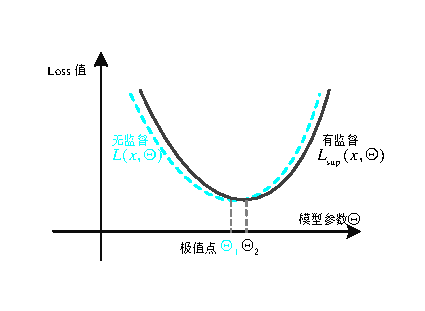
\includegraphics[width=0.8\textwidth]{suploss.pdf}
	\caption{估计校正的的直观阐释示意图}
	\label{Fig:suploss}
\end{figure}
%*******************************

图\ref{Fig:suploss}提供了一个阐释性的例子,固定训练样本$x$,损失值可以看作模型参数$\Theta$的函数。如果,对于所有的模型参数$\Theta$的可能取值,无监督损失函数和有监督损失函数非常接近,那么它们的极值点$\Theta_1$和$\Theta_2$也非常接近,即在无监督数据集中学到接近于有监督数据的模型参数。

需要注意的是,无监督损失和有监督损失的一致性往往以样本数量$N\rightarrow \infty$为前提条件,这是一个理想的情况,在现实中难以实现,有限的样本数量导致估计误差的产生。在有限样本时,$\mathcal{L}_\textsc{~Bcl}$的估计误差具体体现在三个方面:(1)经验分布函数$\hat{\Phi}_\textsc{Un}(\hat{x})$的估计误差,它是未知的分布函数${\Phi}_\textsc{Un}(\hat{x})$的估计;(2) $\alpha$的估计误差,它是编码器的宏AUC估计;(3)重要性采样的估计误差,它是真负样本的相似度分数期望值的估计。由于涉及因素众多,本章不讨论$\mathcal{L}_\textsc{~Bcl}$估计误差的解析表达式。但是,可以明确的是,较大的N值可以使得上述三个误差都减小,进而$\mathcal{L}_\textsc{~Bcl}$的估计误差会确定性地减小。在数值实验部分也印证了这个结论。此外,较大地N值会推高互信息地下界。因此,在实践中,在GPU显存可承受的范围内,应该选择一个尽可能大的N值。

%%*******************************
%\begin{figure*}[!]
%	\centering
%	\subfloat[Fixed $\alpha$ with different $\beta$ settings.]
%	{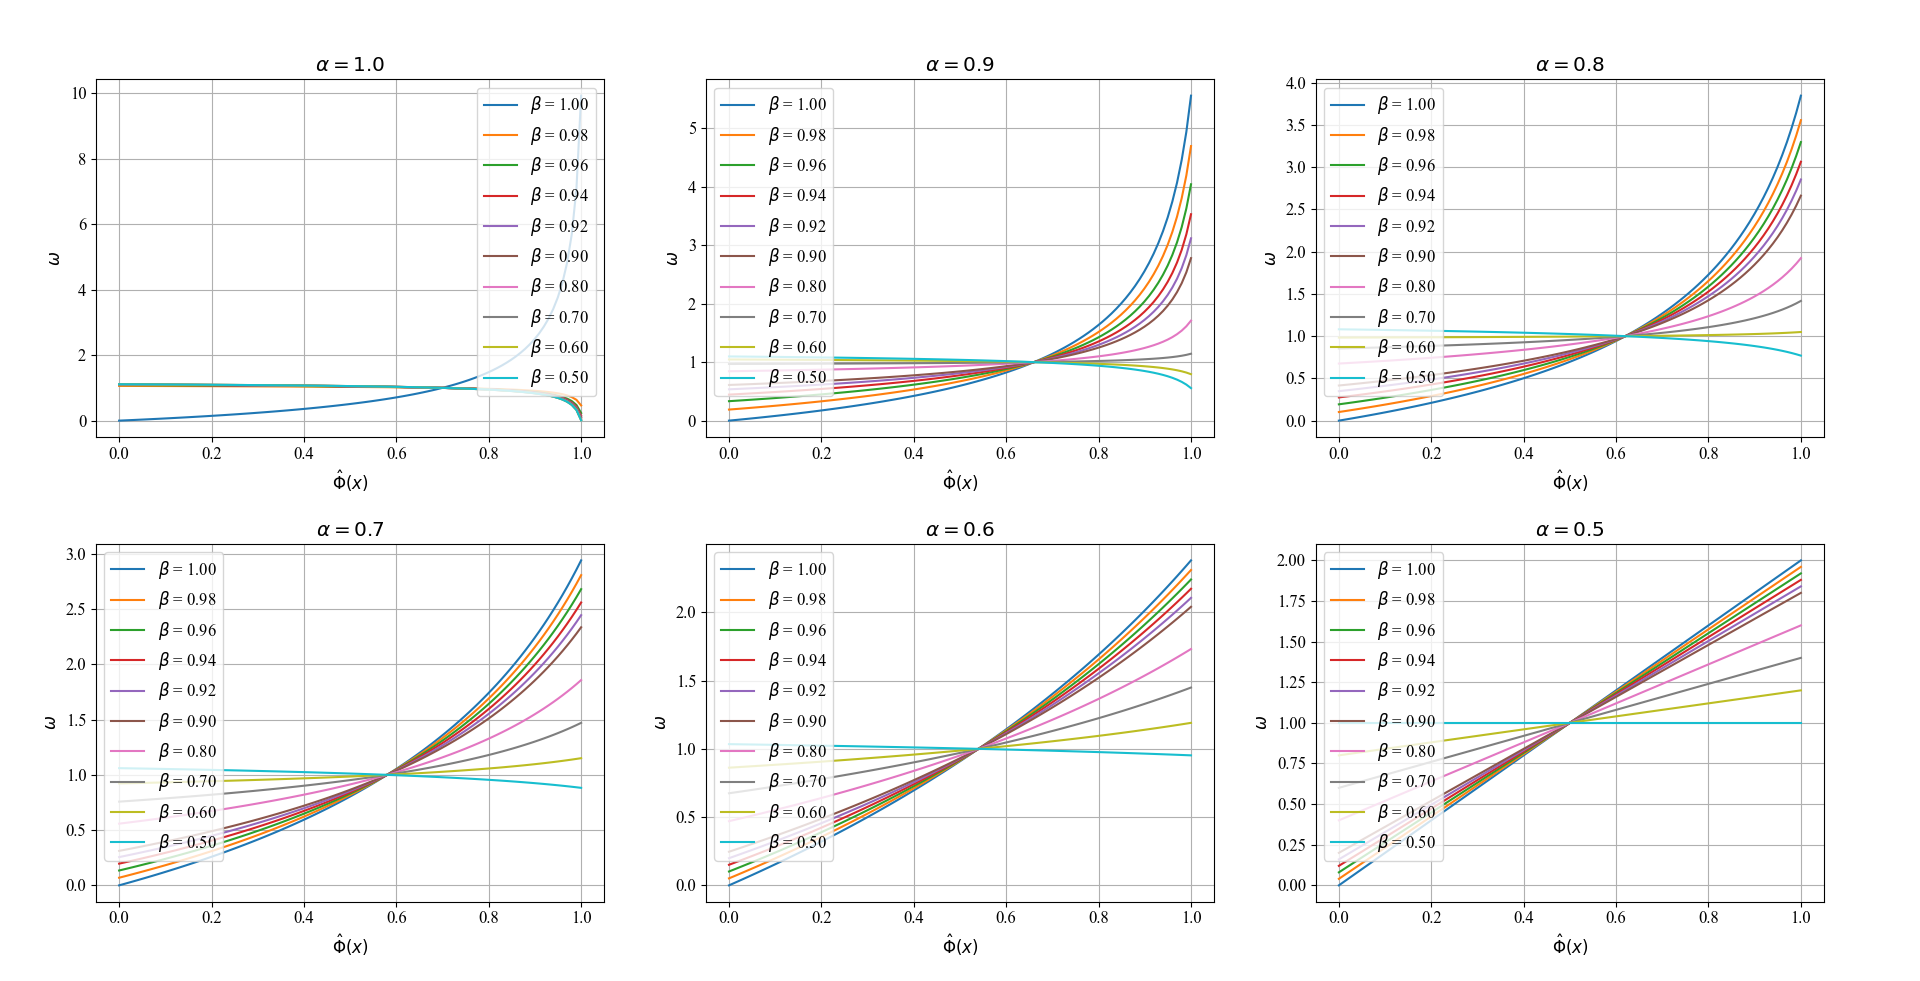
\includegraphics[width=1\textwidth, height=0.5\hsize]{omega_fixalpha.png}\label{fig: omega_a}}\hspace{0.1cm}
%	\subfloat[Fixed $\beta$ with different $\alpha$ settings.]
%	{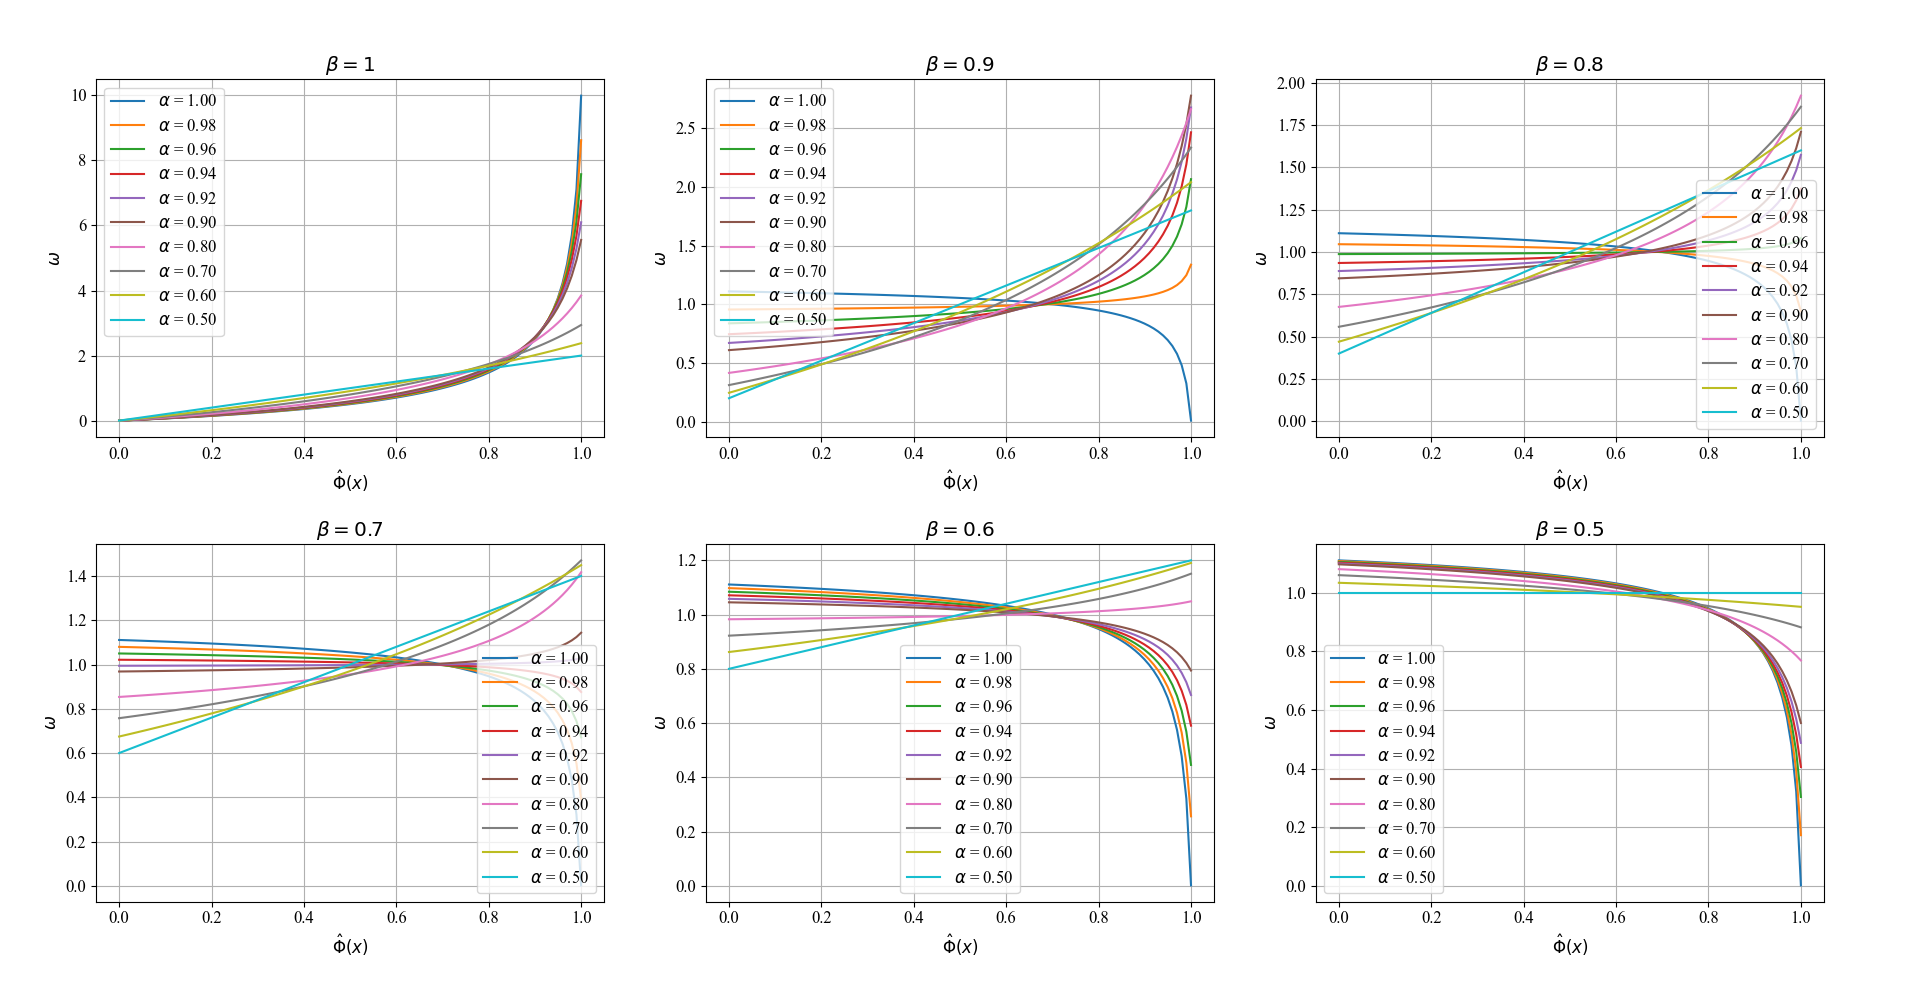
\includegraphics[width=1\textwidth, height=0.5\hsize]{omega_fixbeta.png}\label{fig:omega_b}}
%	\caption{This figure illustrates how the weight $\omega$ changes with respect to $\hat{\Phi}_{\textsc{Un}} (\hat{x})$ under various settings of $\alpha$ and $\beta$, where  $\tau^+$ is fixed at 0.1. X-axis is the empirical C.D.F function $\hat{\Phi}_{\textsc{Un}}$ of unlabeled samples. A value of $\hat{\Phi}_{\textsc{Un}}(\hat{x})=1$ indicates that the instance is the nearest to the anchor, i.e., the highest scored sample. The x-axis can be understood as the hardness level of the samples, with values closer to 1 indicating higher hardness level. The y-axis represents the importance weight $\omega$ calculated based on the BCL computation process. Since $\omega$ is calculated in terms of the empirical C.D.F (relative ranking position) rather than an absolute similarity score, leading it more robust to different temperature scaling settings and encoders. Different values of $\alpha$ and $\beta$ provide flexible options for up-weighting or down-weighting negative samples.}
%	\label{fig:omega}
%\end{figure*}
%%*******************************

\section{实验结果及分析}
由于InfoNCE损失在诸多领域的广泛使用,本章的实验考虑仿真数值实验以及真实数据集实验,在真实数据集上的实验包括个性化推荐任务以及图像分类任务。
\subsection{数值实验}
\subsubsection{实验设置}
\newpage
前面提到,BCL是通过重要性加权未标注样本(实际抽样总体)的相似度分数$\sum_{i=1}^N \omega_i \cdot \hat{x}_i$,以近似真负样本(目标抽样总体)的相似度分数的期望值,从而间接地
实现对有监督损失的近似。那么,对真负样本(目标抽样总体)的相似度分数的期望值估计质量的好坏,决定了是否能够获取与监督损失一致的估计量。在数值实验部分,探讨对真负样本(目标抽样总体)的相似度分数的期望值估计质量的好坏,它决定了与监督损失的一致性,也体现了权重$\omega_i$估计质量的好坏。

前面获得了类条件概率密度(目标抽样群体),以及未标注样本的概率密度(实际抽样群体)的抽象表达式。只要给出任意的相似度分数分布$\phi$,就可以获得类条件概率密度及未标注样本的概率密度的具体表达式。从真负例的类条件概率密度中,可以生成真负例的样本,从而得到期望值;类似地,从伪负例类条件概率密度中,可以生成伪负例样本。两个类被的混合构成了观测到的未标注本。按照BCL的计算步骤得到估计值$\sum_{i=1}^N \omega_i \cdot \hat{x}_i$。对比期望值和估计值,可以评估估计质量的好坏。下面介绍样本生成过程。

\subsubsection{样本生成过程}
\textbf{样本生成过程概述:}
为了生成样本,首先随机初始化一个相似度分数分布$\phi$,如均匀分布,高斯分布等。然后就可以生成对应的样本,见图~\ref{fig:generateN}所示,共分为三步:
\par
\textbf{(1)} 以正类先验概率$\tau^+$选择伪负例的标签, 表明一个观测值以$\tau^+$概率来自伪负例$\textsc{Fn}$总体;以负类先验概率$\tau^-=1-\tau^+$选择真负例的标签, 表明一个观测值以$\tau^-$概率来自真负例$\textsc{Tn}$。

\par
\textbf{(2)} 根据所属类别,从类条件概率密度$\phi_{\textsc{Fn}}$ (或 $\phi_{\textsc{Tn}}$)生成随机样本。需要说明的是,即使将$\phi$设置为简单分布,相应的类条件密度$\phi_{\textsc{Fn}}$(或$\phi_{\textsc{Tn}}$)也不再是简单分布。可以使用接受-拒绝采样~\cite{casella2004generalized}技术,只要给出概率密度表达式,就可以生成服从相应分布的样本。具体的技术细节在后面介绍。
%从$\phi_{\textsc{Fn}}$(或$\phi_{\textsc{Tn}}$)中生成样本的细节见算法\ref{Alg:AccRetTN}和算法\ref{Alg:AccRetFN}。
\par
\textbf{(3)} 将生成的样本$\hat{x}$ 映射为 $\exp(\hat{x}/t)$,并混合两个类,作为最终的未标注样本相似度分数观测值。需要说明的是,前面的方法部分没有讨论将观测值$\hat{x}\rightarrow \exp(\hat{x}/t)$的影响,这是因为这是一个严格单调的变换,经过函数映射以后,经验分布函数保持不变:$\Phi_n(\hat{x}) = \Phi_n(\exp(\hat{x}/t))$,因此完全不影响BCL的估计。

重复图~\ref{fig:generateN}描述的过程$N$次,以生成一个锚点的$N$个观测值,并对$M$个锚点重复此过程,就可以得到$M$个锚点所对应的$M$个观测值序列。完整的样本生成过程描述如算法~\ref{Alg:numer}所示。
%*******************************
\begin{figure*}[!]
	\centering
	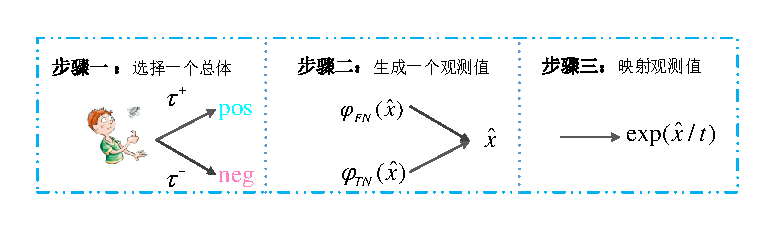
\includegraphics[width=\textwidth]{numerical.pdf}
	\caption{未标注样本相似度分数生成过程示意图}
	\label{fig:generateN}
\end{figure*}
%*******************************
\begin{algorithm}[!]
	\small
	\counterwithin{algorithm}{chapter}
	\SetKwInput{KwIn}{输入}  %<---细节与重点
	\SetKwInput{KwOut}{输出}  %<---细节与重点
	\SetAlgoLined
	\caption{未标注样本相似度分数观测值生成过程}\label{Alg:numer}
	\KwIn{参数$\alpha$,温度系数$t$,未标注样本数量$N$,锚点个数$M$。 }
	\KwOut{未标注样本观测值$\hat{x}$及其对应的标签。}
	\BlankLine
	\For{锚点 $m=1, 2, ..., M$}{
		~~$\backslash$$\backslash$ \textit{选定一个任意参数的相似度分数分布$\phi$} \\
		随机选择$[a,b] \subseteq [-1/t^2, 1/t^2]$;\\
		设定$\phi\sim U(a,b) $; 
		
		\For{负例 $ j=1, 2, ..., N$}{
			~~$\backslash$$\backslash$ \textit{step1:选择一个总体} \\
			~~$p$ = random.uniform(0,1);
			
			\If{$p \leq \tau^+$}{~~$\backslash$$\backslash$ \textit{step2:从伪负例类条件分布 $\phi_{\textsc{Fn}}$中生成样本} 
				
				~~$\hat{x}_j$ = AccRejetSamplingFN($\phi_{\textsc{Fn}}$);\\
				label = False;
			}
		
			\Else{~~$\backslash$$\backslash$ \textit{step2:从真负例类条件分布$\phi_{\textsc{Tn}}$}中生成样本\\
				~~$\hat{x}_j$ = AccRejetSamplingTN($\phi_{\textsc{Tn}}$); \\
				label = True;
			}
			~~$\backslash$$\backslash$ \textit{step3:函数映射} \\
			$\hat{x}_j = \exp(\hat{x}_j/t)$; \\
			收集$\hat{x}_j$数值及标签;
		}
	}
	\KwResult{未标注样本观测值$\hat{x}$及其对应的标签。}
\end{algorithm}

相似度分数分布$\phi$可以是任意的,也称为建议分布(Proposal Distribution)。对于投影到半径为$1/t$的超球面的表示,相似度观测值的值域为$[-1/t^2, 1/t^2]$。为了方便地控制观测值在其理论最小和最大区间$[-1/t^2,1/t^2]$内,并且先前的研究表明,对比损失在渐近情况下优化了负样本的均匀性~\cite{Wang:2020:ICML},将$\phi$设置为$U(a,b)$以进行数值实验,其中$-1/t^2\leq a \leq b \leq 1/t^2$是针对每个锚点随机选择的。具体而言,原始区间设置为$a=-0.5$,$b=0.5$,并使用$\gamma \in [0,1]$来控制从原始区间的变异程度。$\gamma=1$时,不同锚点之间参数$a,b$参数变异程度最大;$\gamma=0$时,不同的参数$a,b$参数变异程度最小,都为$a=-0.5$,$b=0.5$。

%更规范的$\hat{x}$样本生成过程见如下随机过程描述。
%\begin{definition}[样本函数空间]
%	考虑一个定义在$\mathcal{X} \times \Omega$上的两个变量的函数$X(x,e)$。对于一个锚点$x\in \mathcal{X}$,函数$X(x,e)$是与样本$x_i$相关的随机变量;对于固定的$e\in \Omega$,$X(x,e)$是与锚点相关的样本函数。称${X(x,e): x\in \mathcal{X}, e\in \Omega}$为样本函数空间。
%\end{definition}
%在样本函数空间中,一个锚点$x$确定了分布$\phi$的参数。由于对不同的锚点,$\phi$不要求相同,它模拟了不同锚点可能导致不同观测分布的情况。
%得到了对应于样本函数空间${X(x,e): x\in \mathcal{X}, e\in \Omega}$中的经验观测的集合${\exp(\hat{x}_{mi}/t): m=1,...,M, i=1,\cdots N}$。

\textbf{接受-拒绝采样实现}:生成样本的第二步(图~\ref{fig:generateN}),涉及从从类条件密度$\phi_{\textsc{Tn}}(\hat{x})$生成相应的样本$\hat{x}$,使得$\hat{x} \sim \phi_{\textsc{Tn}}(\hat{x})$。由于类条件概率密度的表达式通常很复杂,不再是简单的均匀分布或者高斯分布,难以直接采样。本节采用标准的接受-拒绝采样方法实现,其基本思想是从建议分布$\phi$中生成样本$\hat{x}$,并以接受概率$p_{\textsc{Tn}}$接受该样本。为了计算接受概率$p_{\textsc{Tn}}$,首先将$\phi_{\textsc{Tn}}(\hat{x})$写为$\phi$的函数
\begin{eqnarray}
	\phi_{\textsc{Tn}}(\hat{x}) &=& \alpha \phi_{(1)}(\hat{x}) + (1-\alpha)\phi_{(2)}(\hat{x}) \nonumber\\
	&=& [2\alpha+(2-4\alpha)\Phi(\hat{x})]\phi(\hat x), \nonumber
\end{eqnarray}
其中$\Phi(\hat{x})$是$\phi(\hat{x})$对应的累积分布函数。接下来,寻找一个最小值$c$满足如下不等式
\[c \cdot \phi(\hat{x}) \geq \phi_{\textsc{Tn}}(\hat{x}),\]
即
\[c \cdot \phi(\hat{x}) \geq  [2\alpha+(2-4\alpha)\Phi(\hat{x})]\phi(\hat x).\]
因此
\begin{eqnarray}
	c &=& min [2\alpha+(2-4\alpha)\Phi(\hat{x})], \Phi(\hat{x}) \in [0,1]\nonumber\\
	&=&2\alpha, \nonumber
\end{eqnarray}
最小值$c$在$\Phi(\hat{x})=0$时取得,由于$2-4\alpha \leq 0$。因此接受概率
\begin{eqnarray}
	p_{\textsc{Tn}} &=& \frac{\phi_{\textsc{Tn}}(\hat{x})}{c \cdot \phi(\hat{x}) } \nonumber \\
	&=& [\alpha + (1-2 \alpha)\cdot \Phi(\hat{x})] /\alpha \nonumber
\end{eqnarray}
从建议分布$\phi(\hat{x})$生成的样本$\hat{x}$以概率$p_{\textsc{Tn}}$被接受,得到了服从分布$ \phi_{\textsc{Tn}}(\hat{x})$的样本,如算法~\ref{Alg:AccRetTN}描述。
\begin{algorithm}[!]
	\counterwithin{algorithm}{chapter}
	\SetKwInput{KwIn}{输入}  %<---细节与重点
	\SetKwInput{KwOut}{输出}  %<---细节与重点
	\SetAlgoLined
	\small
	\caption{~生成服从$\phi_{\textsc{Tn}}$分布的样本的接受拒绝采样算法AccRejetSamplingTN($\phi_{\textsc{Tn}}$)}\label{Alg:AccRetTN}
	\KwIn{参数$\alpha$, 建议分布$\phi$。 }
	\KwOut{服从分布$\phi_{\textsc{Tn}}$的样本$\hat{x}$。}
	\BlankLine
	~~从分布$\phi$中采样一个随机样本$\hat{x}_j$;\\
	cdf = $\int_{-\infty}^{\hat{x}_j} \phi(t)dt$; \\
	u = random.uniform$(0,1)$; 
	
	\While{u $ > [\alpha + (1-2 \alpha)\cdot cdf] /\alpha ~$~ }{
		~~$\backslash$$\backslash$ \textit{样本$\hat{x}_j$被拒绝,重新采样} \\
		从分布$\phi$中采样一个随机样本$\hat{x}_j$;\\
		cdf = $\int_{-\infty}^{\hat{x}_j} \phi(t)dt$; \\
		u = random.uniform$(0,1)$;
	}
	\KwResult{服从分布$\phi_{\textsc{Tn}}$的样本$\hat{x}_j$。}
\end{algorithm}

同样地,对于类条件概率密度$\phi_{\textsc{Fn}}$,接受概率的计算步骤类似,为
\[p_{\textsc{Fn}} = [1 - \alpha + (2 \alpha - 1)\cdot \Phi(\hat{x})] / \alpha \]
从建议分布$\phi(\hat{x})$生成的样本$\hat{x}$以概率$p_{\textsc{Fn}}$被接受,得到了服从分布$ \phi_{\textsc{Fn}}(\hat{x})$的样本,如算法~\ref{Alg:AccRetFN}描述。
\begin{algorithm}[!]
	\counterwithin{algorithm}{chapter}
	\SetKwInput{KwIn}{输入}  %<---细节与重点
	\SetKwInput{KwOut}{输出}  %<---细节与重点
	\SetAlgoLined
	\small
	\caption{~生成服从$\phi_{\textsc{Fn}}$分布的样本的接受拒绝采样算法AccRejetSamplingFN($\phi_{\textsc{Fn}}$)}\label{Alg:AccRetFN}
	\KwIn{参数$\alpha$, 建议分布$\phi$。}
	\KwOut{服从分布$\phi_{\textsc{Fn}}$的样本$\hat{x}$。}
	\BlankLine
	~~从分布$\phi$中采样一个随机样本$\hat{x}_j$;\\
	cdf = $\int_{-\infty}^{\hat{x}_j} \phi(t)dt$; \\
	u = random.uniform$(0,1)$; 
	
	\While{u $ > [1 - \alpha + (2 \alpha - 1)\cdot cdf ] /\alpha ~$~ }{
		~~$\backslash$$\backslash$ \textit{样本$\hat{x}_j$被拒绝,重新采样} \\
		从分布$\phi$中采样一个随机样本$\hat{x}_j$; \\
		cdf = $\int_{-\infty}^{\hat{x}_j} \phi(t)dt$; \\
		u = random.uniform$(0,1)$;
	}
	
	\KwResult{服从分布$\phi_{\textsc{Fn}}$的样本$\hat{x}$。}
\end{algorithm}
\begin{figure}[!]
	\centering
	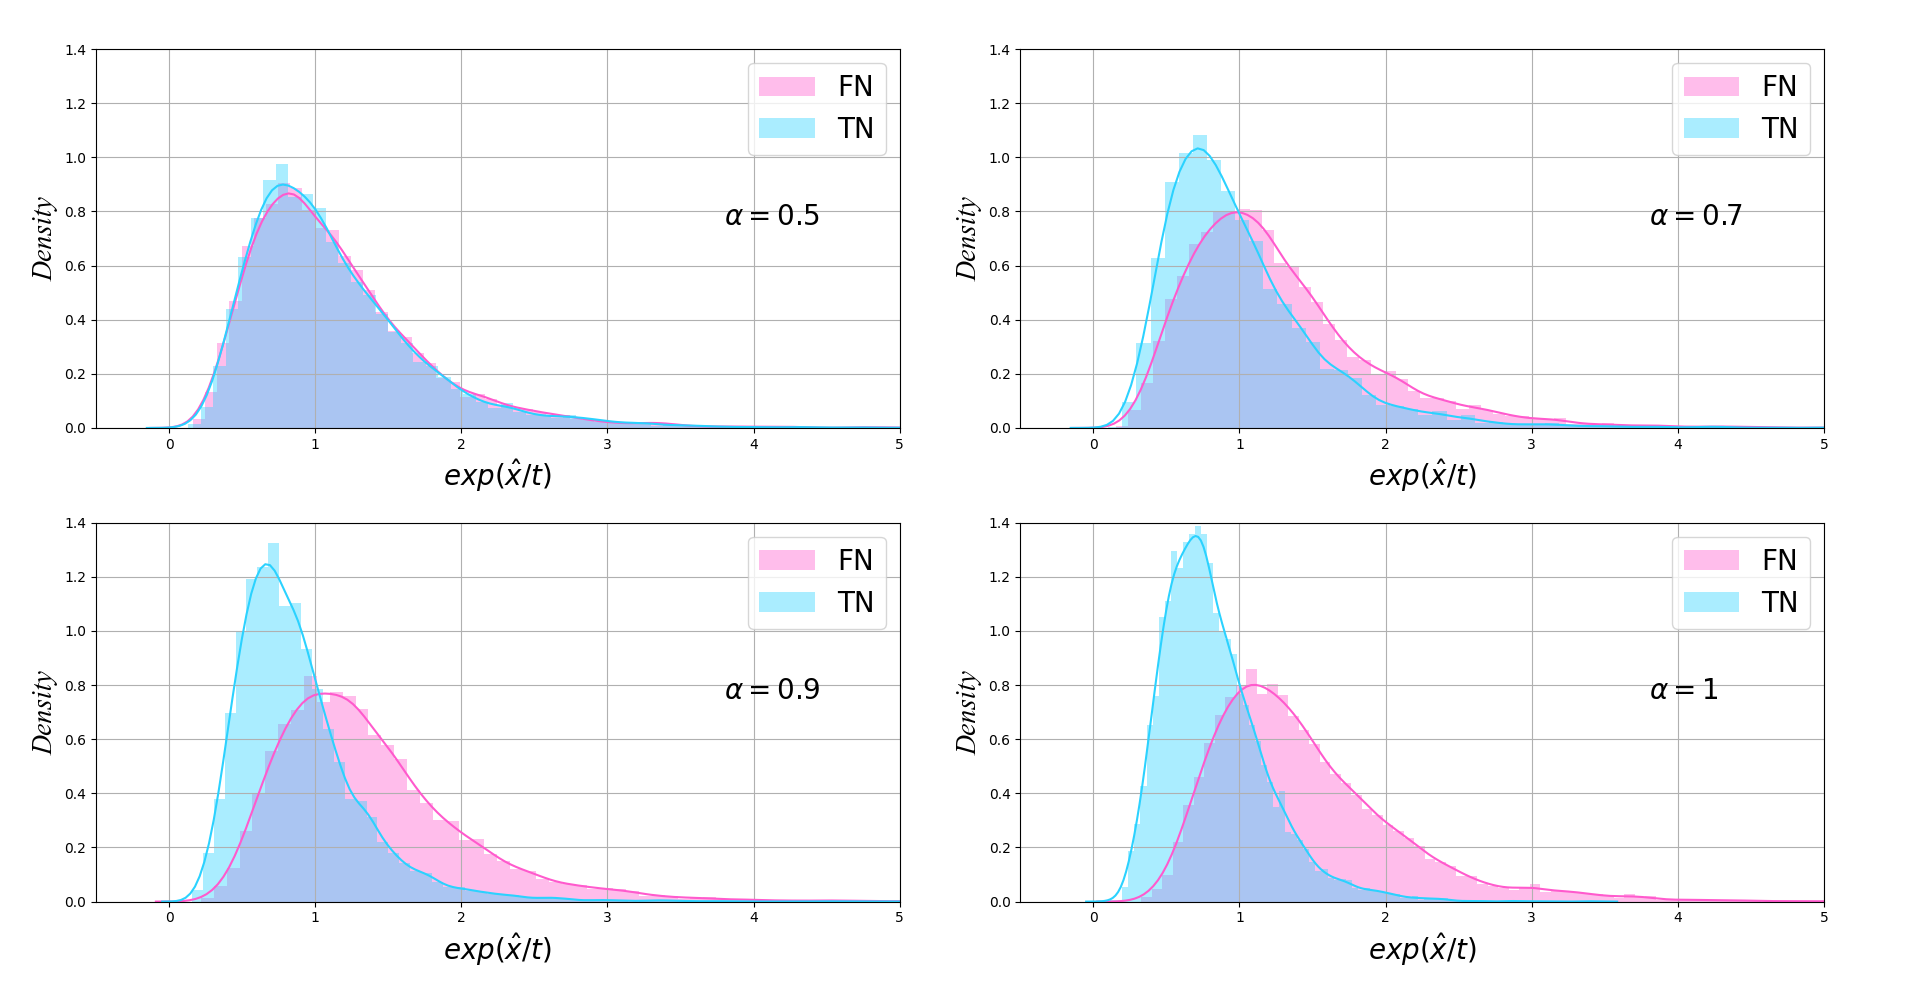
\includegraphics[width=\textwidth]{empiricaldist.png}
	\caption{不同$\alpha$设置下相似度分数的经验分布}
	\label{Fig:empiricaldist}
\end{figure}
\par
根据上述生成过程,图~\ref{Fig:empiricaldist}绘制了生成的样本$\exp(\hat{x}/t)$的经验分布,其中$\phi$设定为标注正态分布,与图~\ref{Fig:theorydist}相对应。其中,$t=2$,$M=1$和$N=20000$。可以看到,图~\ref{Fig:empiricaldist}中的经验分布展现出与使用实际数据集报告的分布~\cite{Robinson:2021:ICLR, Xia:2022:ICML}相似的结构,表明所提出的对样本$\hat{x}$的生成过程描述的有效性。

\subsubsection{对比方法}
在实践中,通常是使用均值作为期望值的经验估计~\cite{Oord:2018:arxiv,Chuang:2020:NIPS,Chen:2020:ICML},因此使用$N$个随机样本中真负例相似度分数的均值作为真值的参考,可以通过如下方式计算
\begin{equation}\label{eq:true}
	\theta_{\textsc{Sup}} = \frac{\sum_{i=1}^N \mathbb{I}(\hat x_i) \cdot \hat{x}_i  }{ \sum_{i=1}^N \mathbb I(\hat{x}_i) },
\end{equation}
其中,$\mathbb{I}(x_i)$是指示函数,如果$\hat{x}_i \in \textsc{Tn}$,则$\mathbb{I}(\hat x_i)=1$;否则,$\mathbb{I}(\hat x_i)=0$,那么式\eqref{eq:true}分子的含义是真负例分数和,分母是真负例的个数,因此式\eqref{eq:true}的含义是真负例分数均值。

对比方法如下:
\begin{eqnarray}
	&&\hat{\theta}_\textsc{Biased} =\frac{1}{N} \sum_{i=1}^{N} \hat{x}_i \label{5Eq:BiasedEstimator} \\
	&&\hat{\theta}_\textsc{Dcl} =  \frac{1}{N\tau^-}  (\sum_{i=1}^{N} \hat{x}_i - N\tau^+ \cdot \frac{\sum_{j=1}^{K} \hat{x}_j^+}{K} ) \label{5Eq:DCLEstimator} \\
	&& \hat\theta_\textsc{Bcl} =\frac{1}{N}  \sum_{i=1}^N \omega_i \cdot \hat{x}_i\label{5Eq:BCLEstimator}
\end{eqnarray}
式~\eqref{5Eq:BiasedEstimator}是标准的InfoNCE损失\cite{Oord:2018:arxiv}对应的估计量,含义为未标注样本的相似度分数均值。式\eqref{5Eq:DCLEstimator}是DCL\cite{Chuang:2020:NIPS}方法所对应的估计量,其含义在第\ref{cha:fourthsection}章的实验部分介绍了,这里不再赘述。此外HCL~\cite{Robinson:2021:ICLR}方法是从任务需求的角度考量,而非从统计量优良性的角度考量。由于上加权困难样本,过度高估真负例分数的均值,在数值实验中不考虑该对比方法。类似地,式\eqref{5Eq:BCLEstimator}中,设定$\beta=0.5$,即不考虑额外的硬负例挖掘任务,只考虑BCL方法估计量的优良性。
%*******************************
\begin{figure*}[h!]
	\centering
	\subfloat[$\alpha$(即编码器$f$性能)的影响]
	{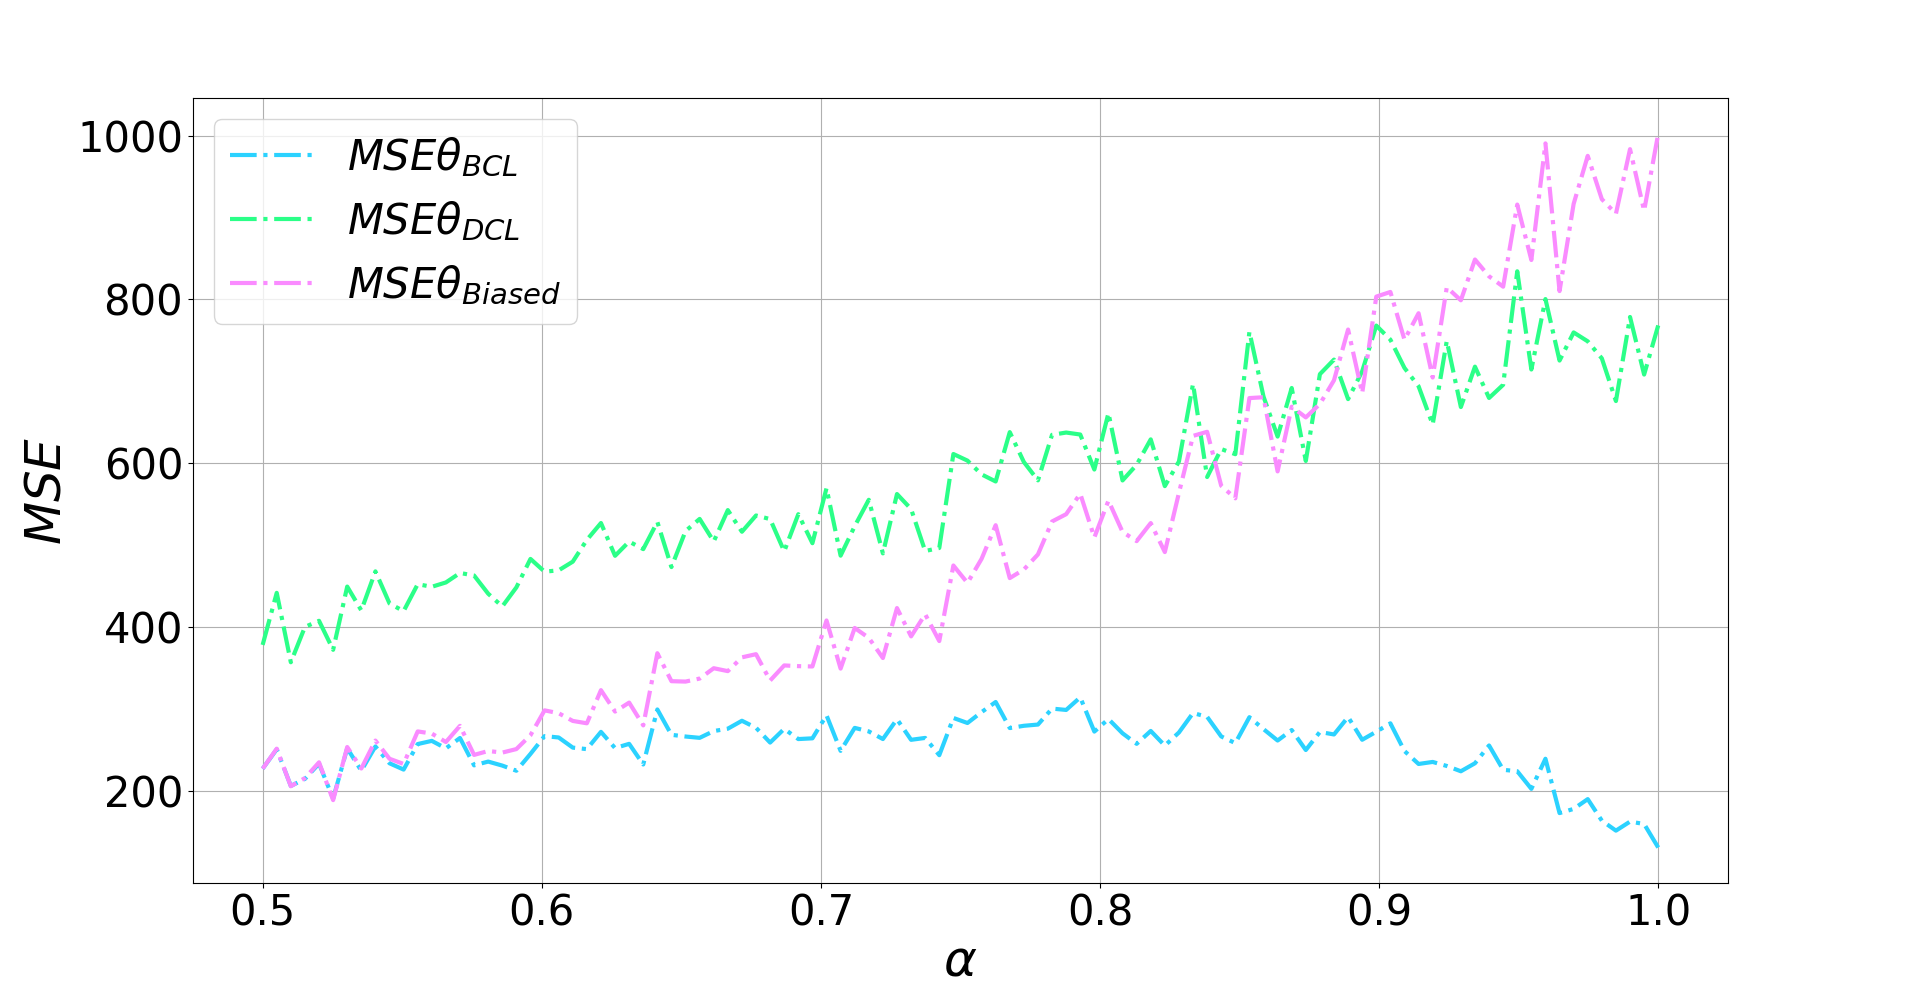
\includegraphics[width=0.5\textwidth, height=0.3\hsize]{numer_alpha.png}\label{fig:msealpha}}
	\subfloat[负例个数N的影响]
	{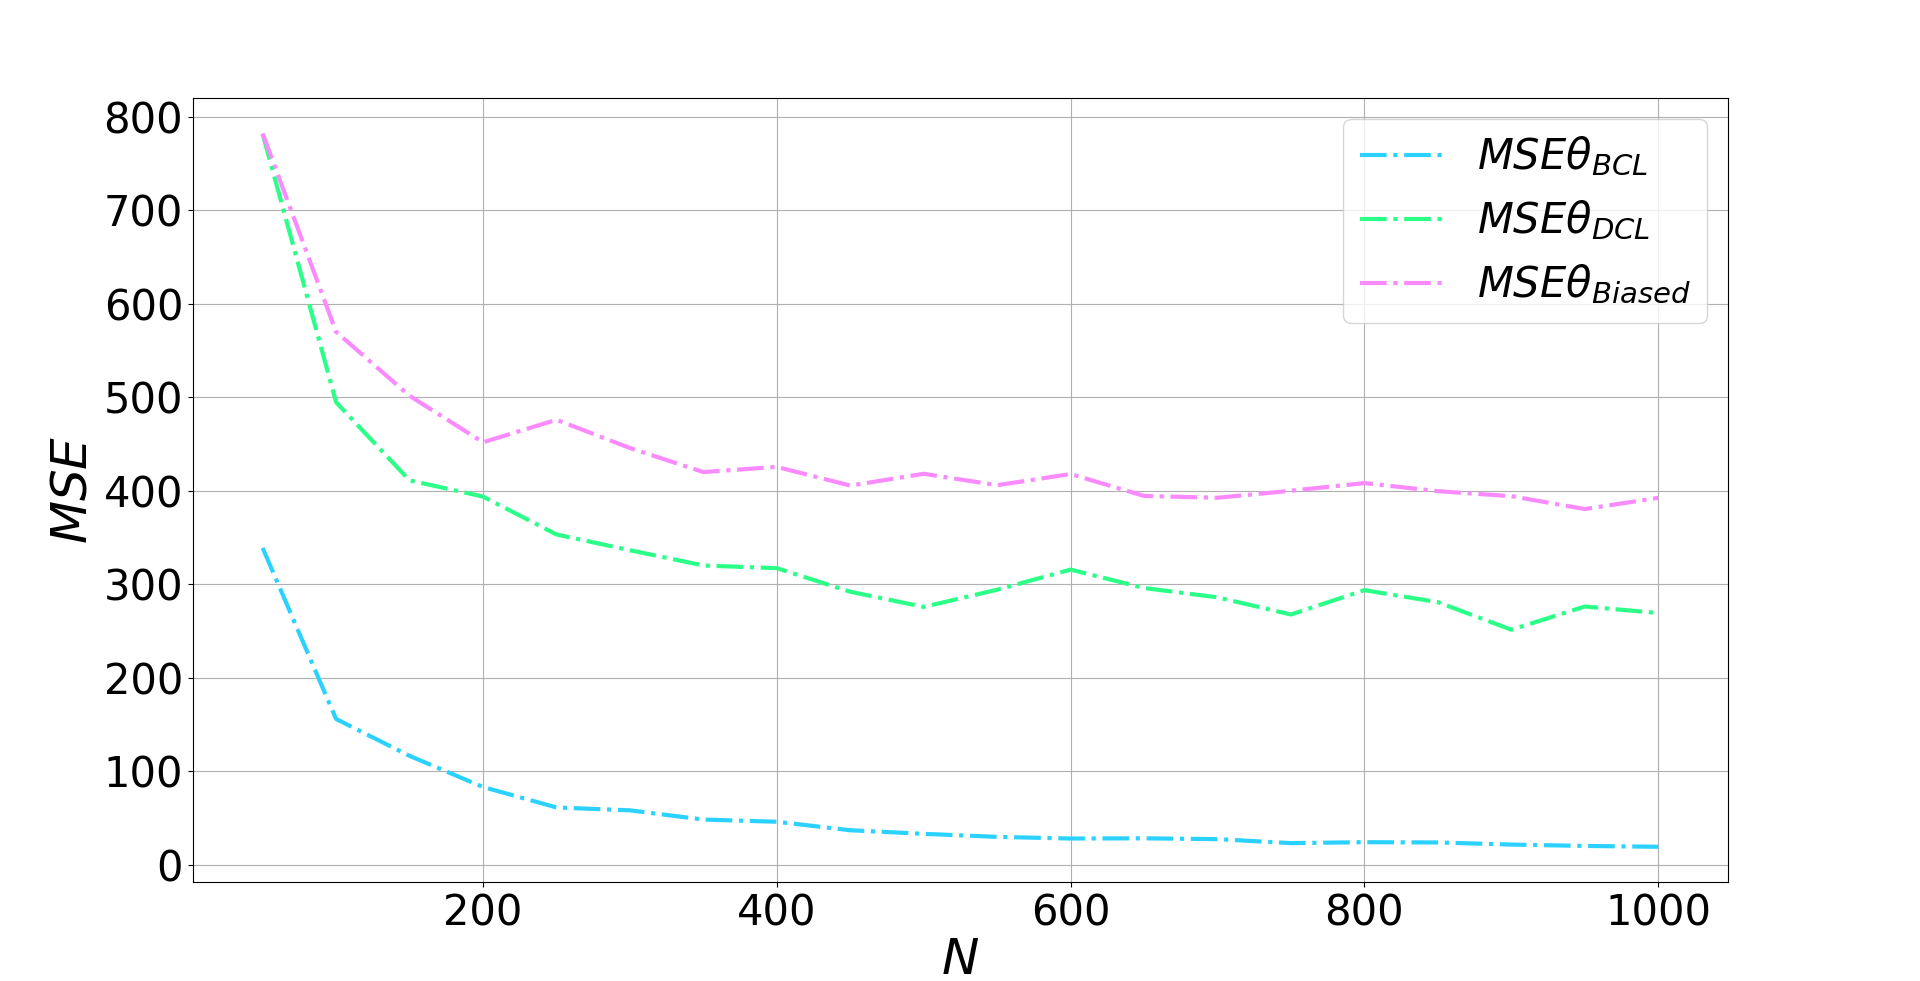
\includegraphics[width=0.5\textwidth, height=0.3\hsize]{numer_N.png}\label{fig:mseN}}\\
	\subfloat[类先验概率的影响]
	{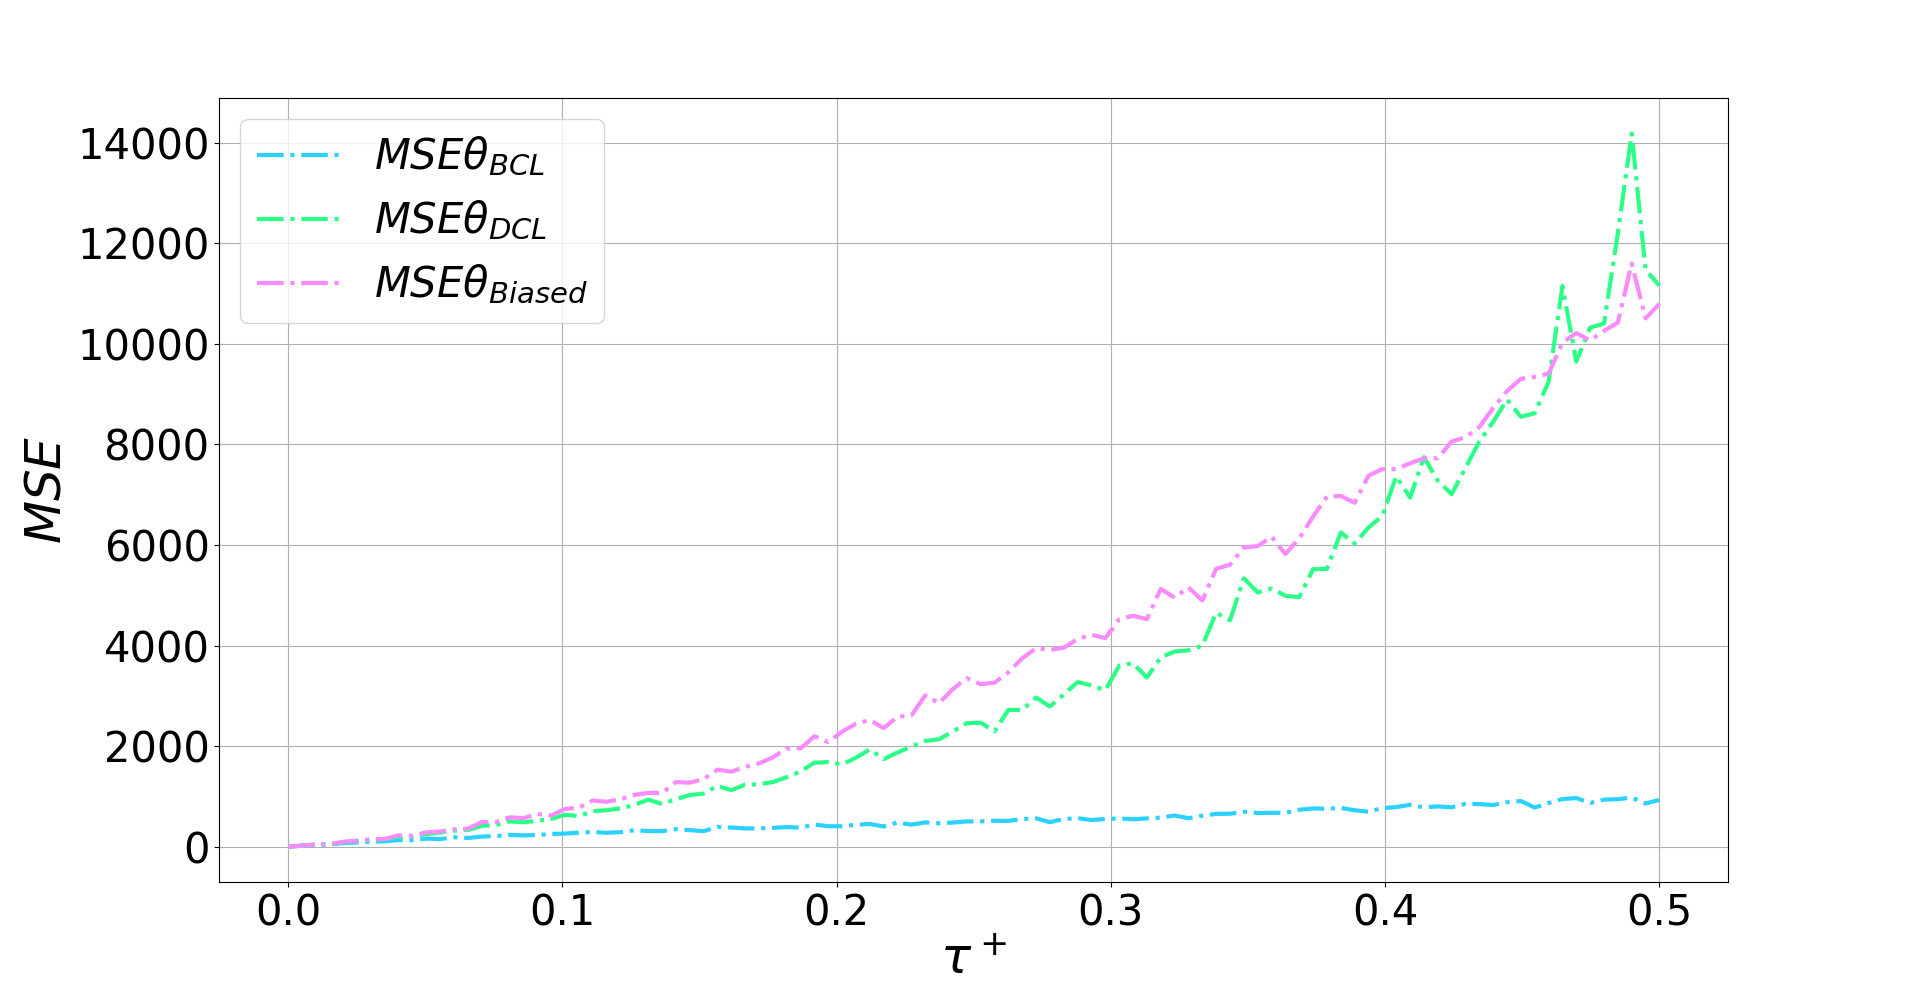
\includegraphics[width=0.5\textwidth, height=0.3\hsize]{numer_tau.png}\label{fig:msetau}}
	\subfloat[不同锚点的$\phi$变异程度的影响]
	{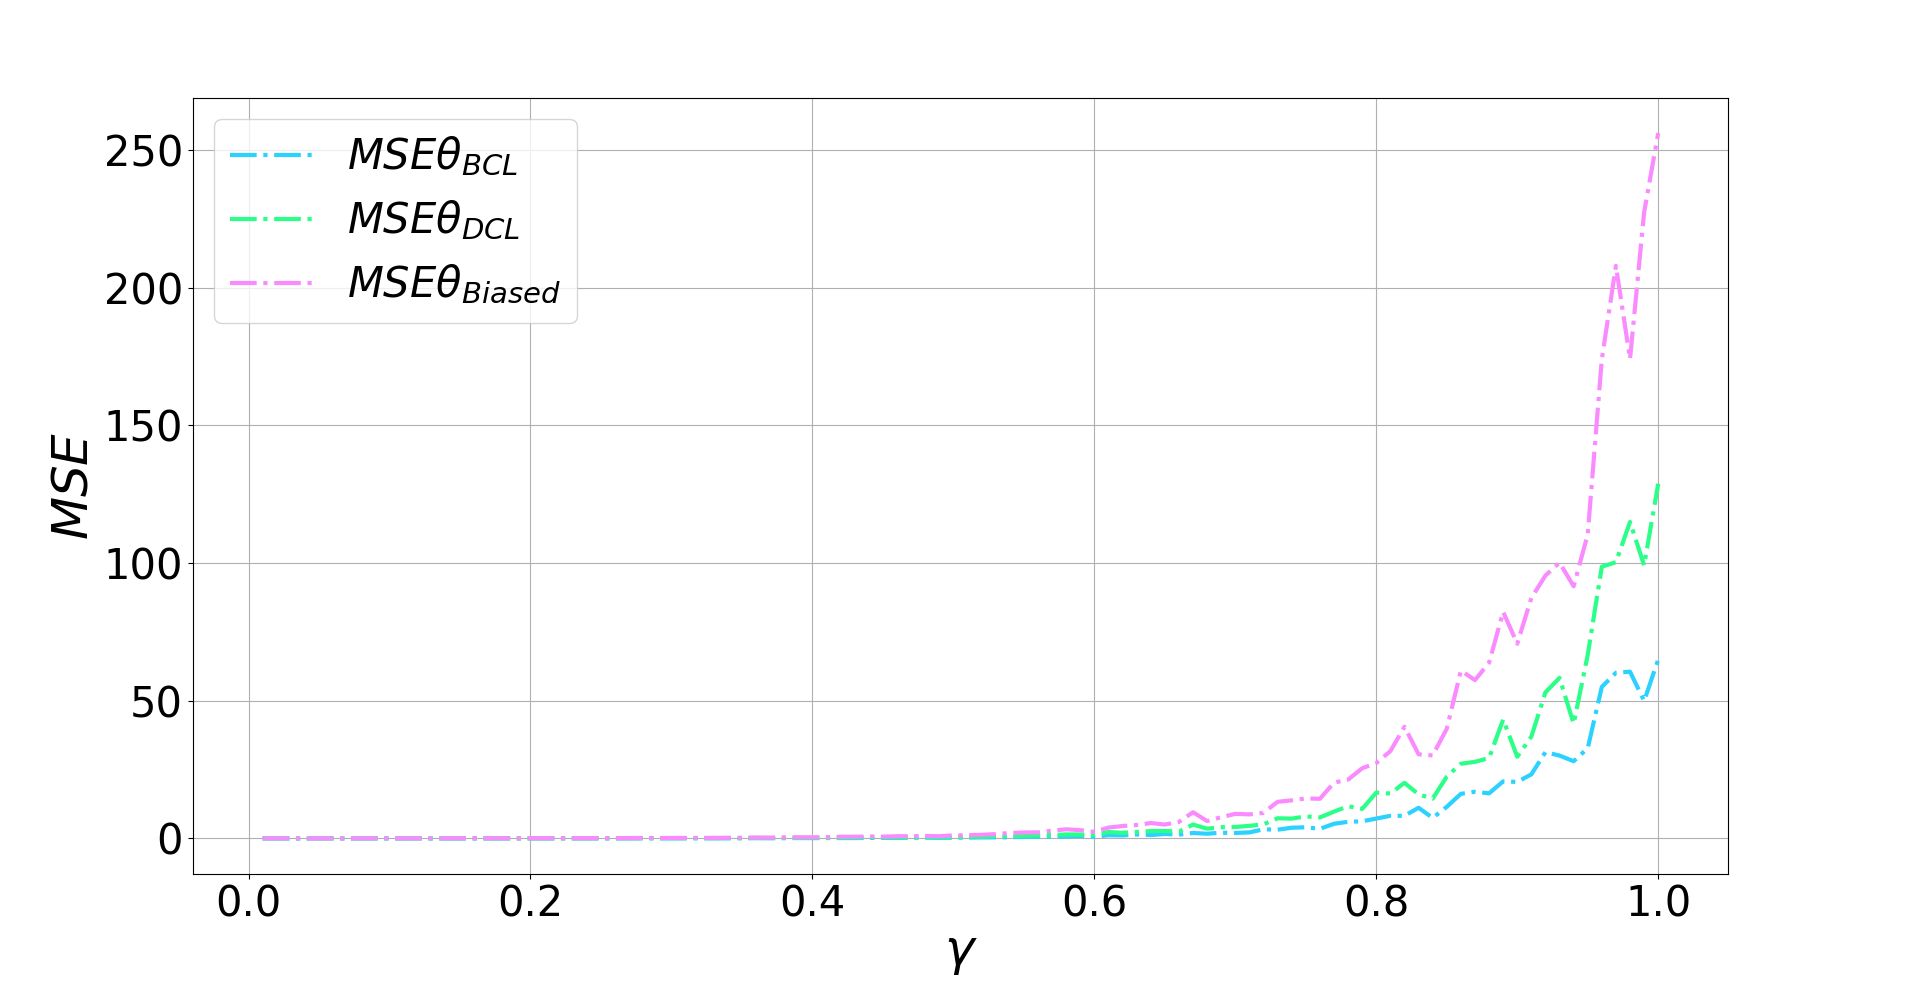
\includegraphics[width=0.5\textwidth, height=0.3\hsize]{numer_gamma.png}\label{fig:msegamma}}\\
	\subfloat[温度放缩系数$t$的影响]
	{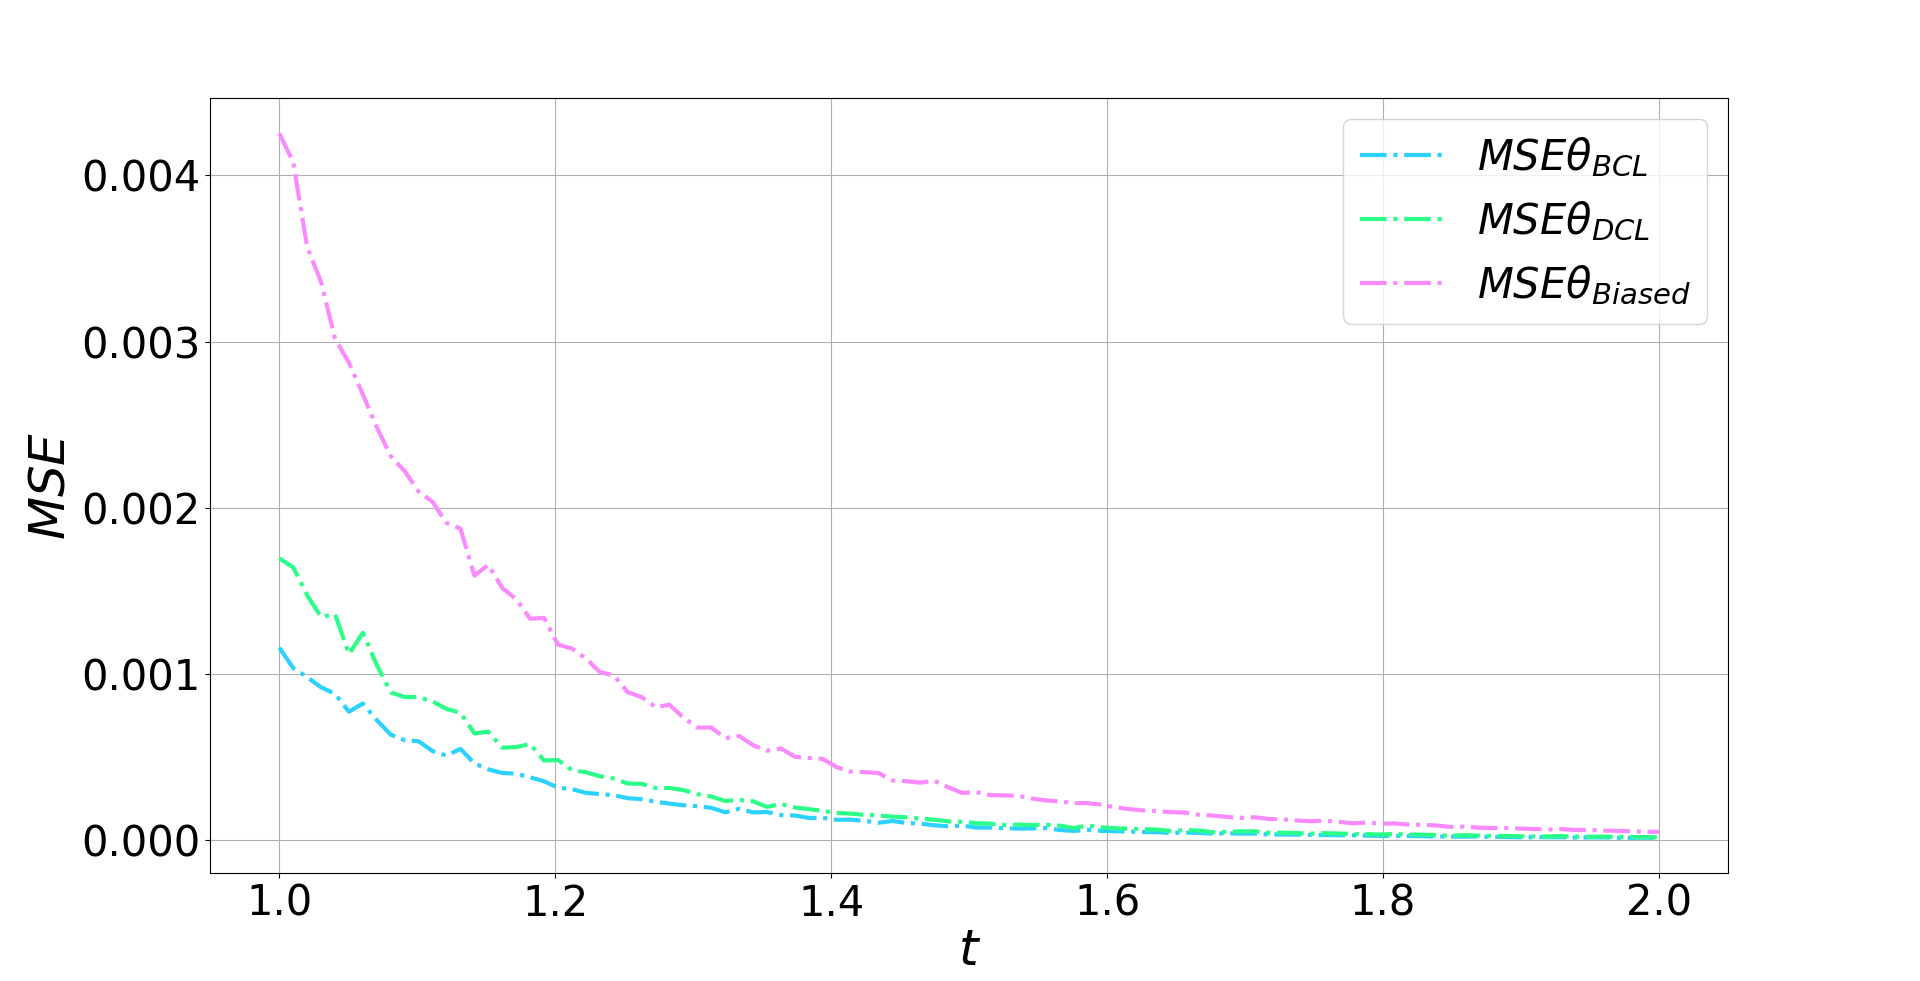
\includegraphics[width=0.5\textwidth, height=0.3\hsize]{numer_t.png}\label{fig:mset}}
	\subfloat[锚点数量M的影响]
	{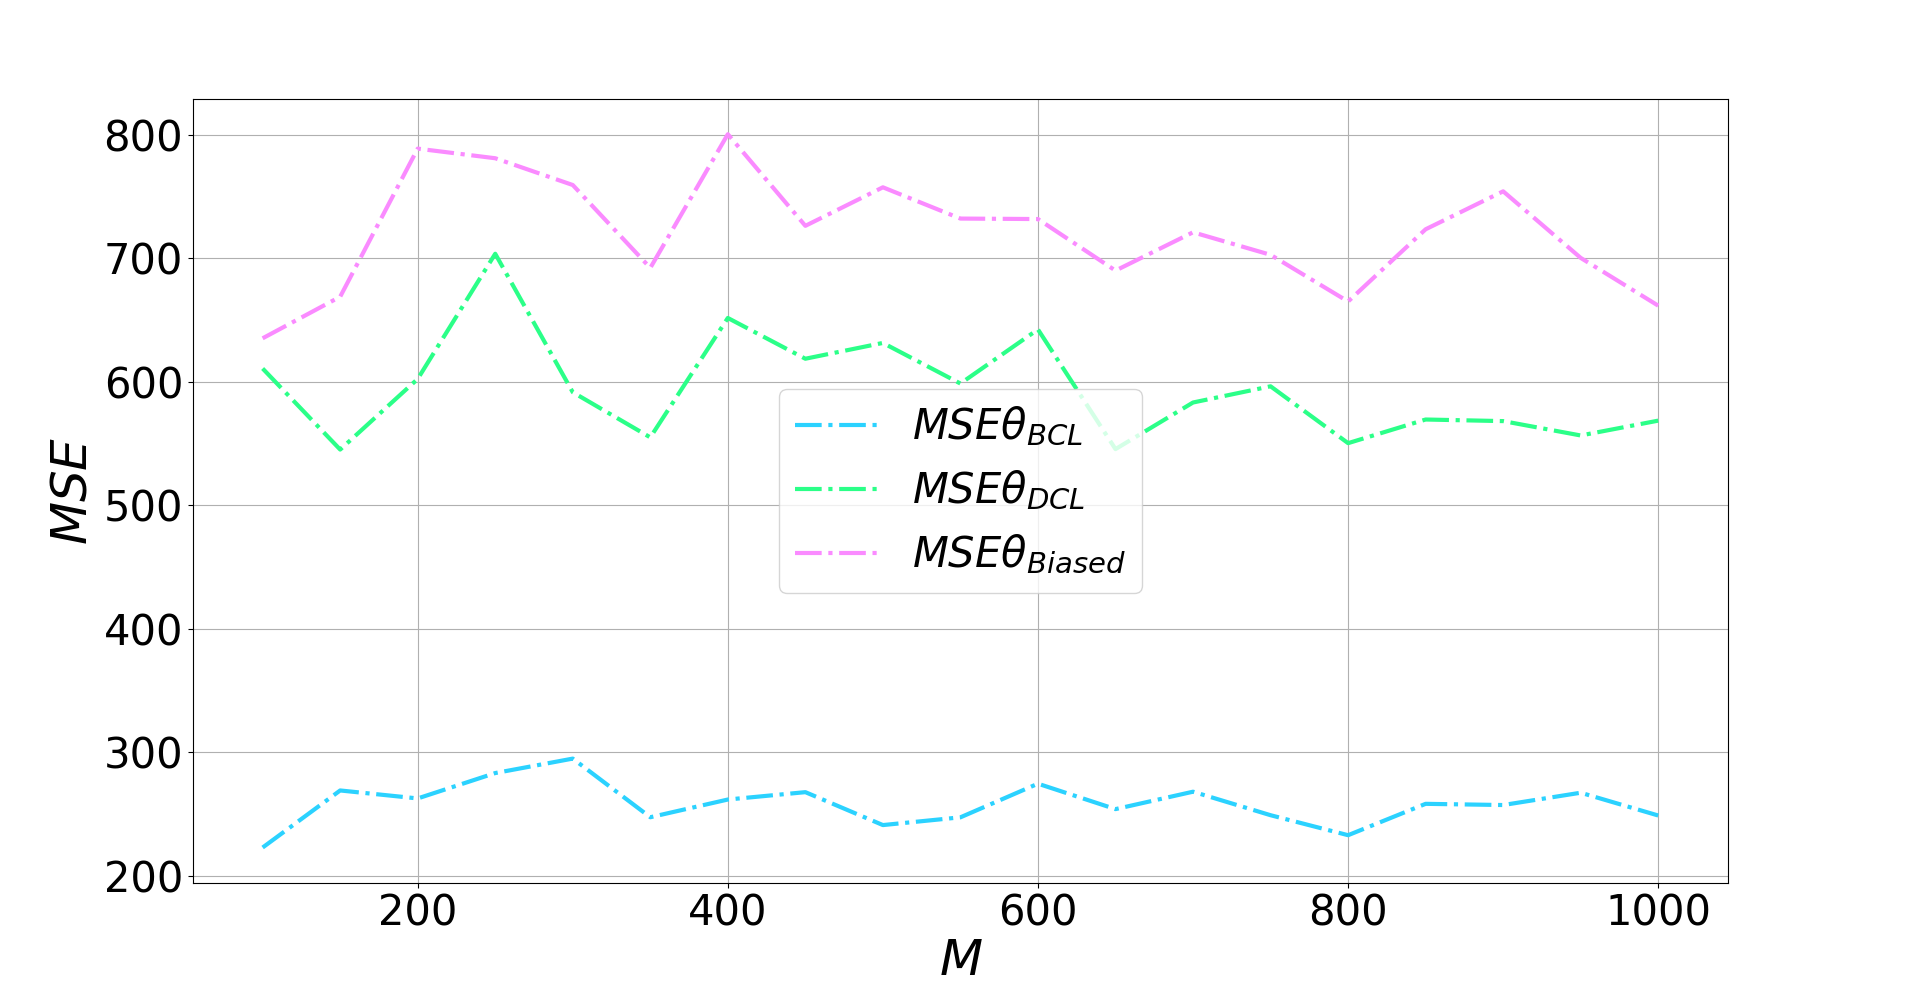
\includegraphics[width=0.5\textwidth, height=0.3\hsize]{numer_M.png}\label{fig:mseM}}
	\caption{不同参数设置下估计量的均方误差比较}
	\label{Fig:MSE}
\end{figure*}
%*******************************

%*******************************
\begin{figure}[h!]
	\centering
	\subfloat[]
	{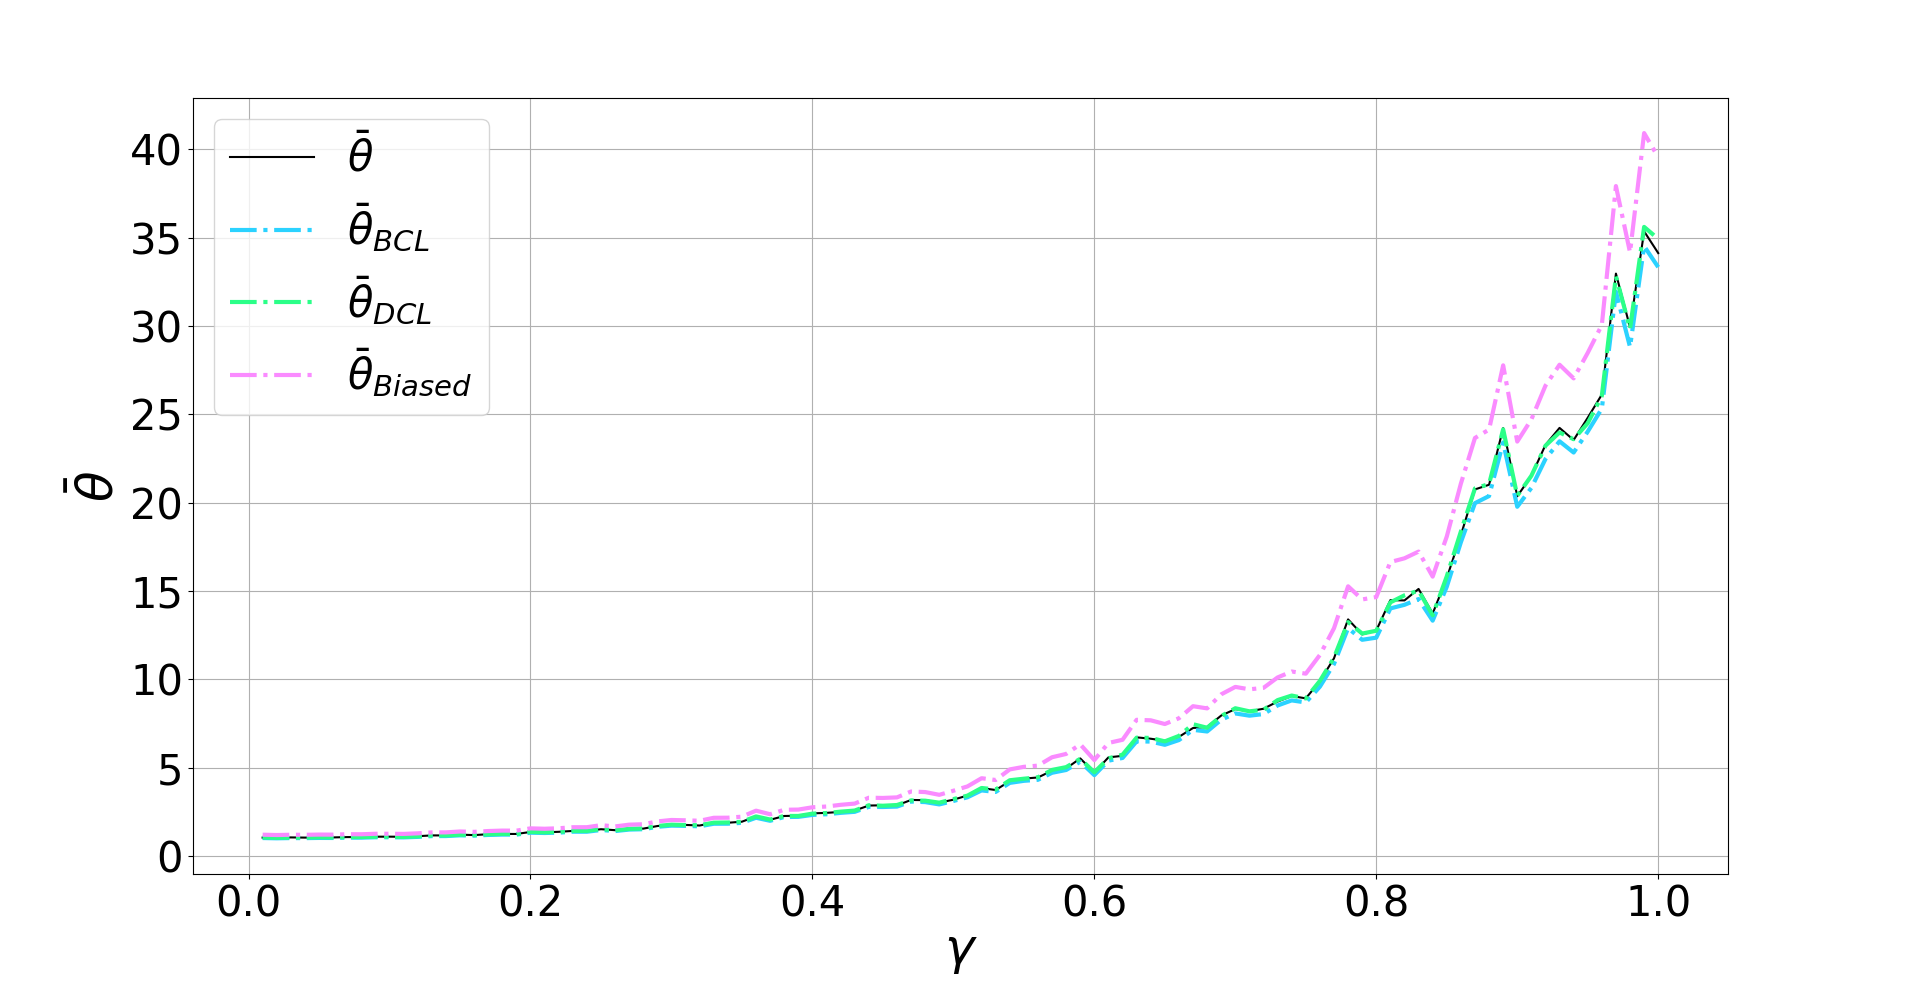
\includegraphics[width=0.49\textwidth, height=0.3\hsize]{numer_bargamma.png}\label{fig: numerbar_gamma}}\hspace{0.1cm}
	\subfloat[]
	{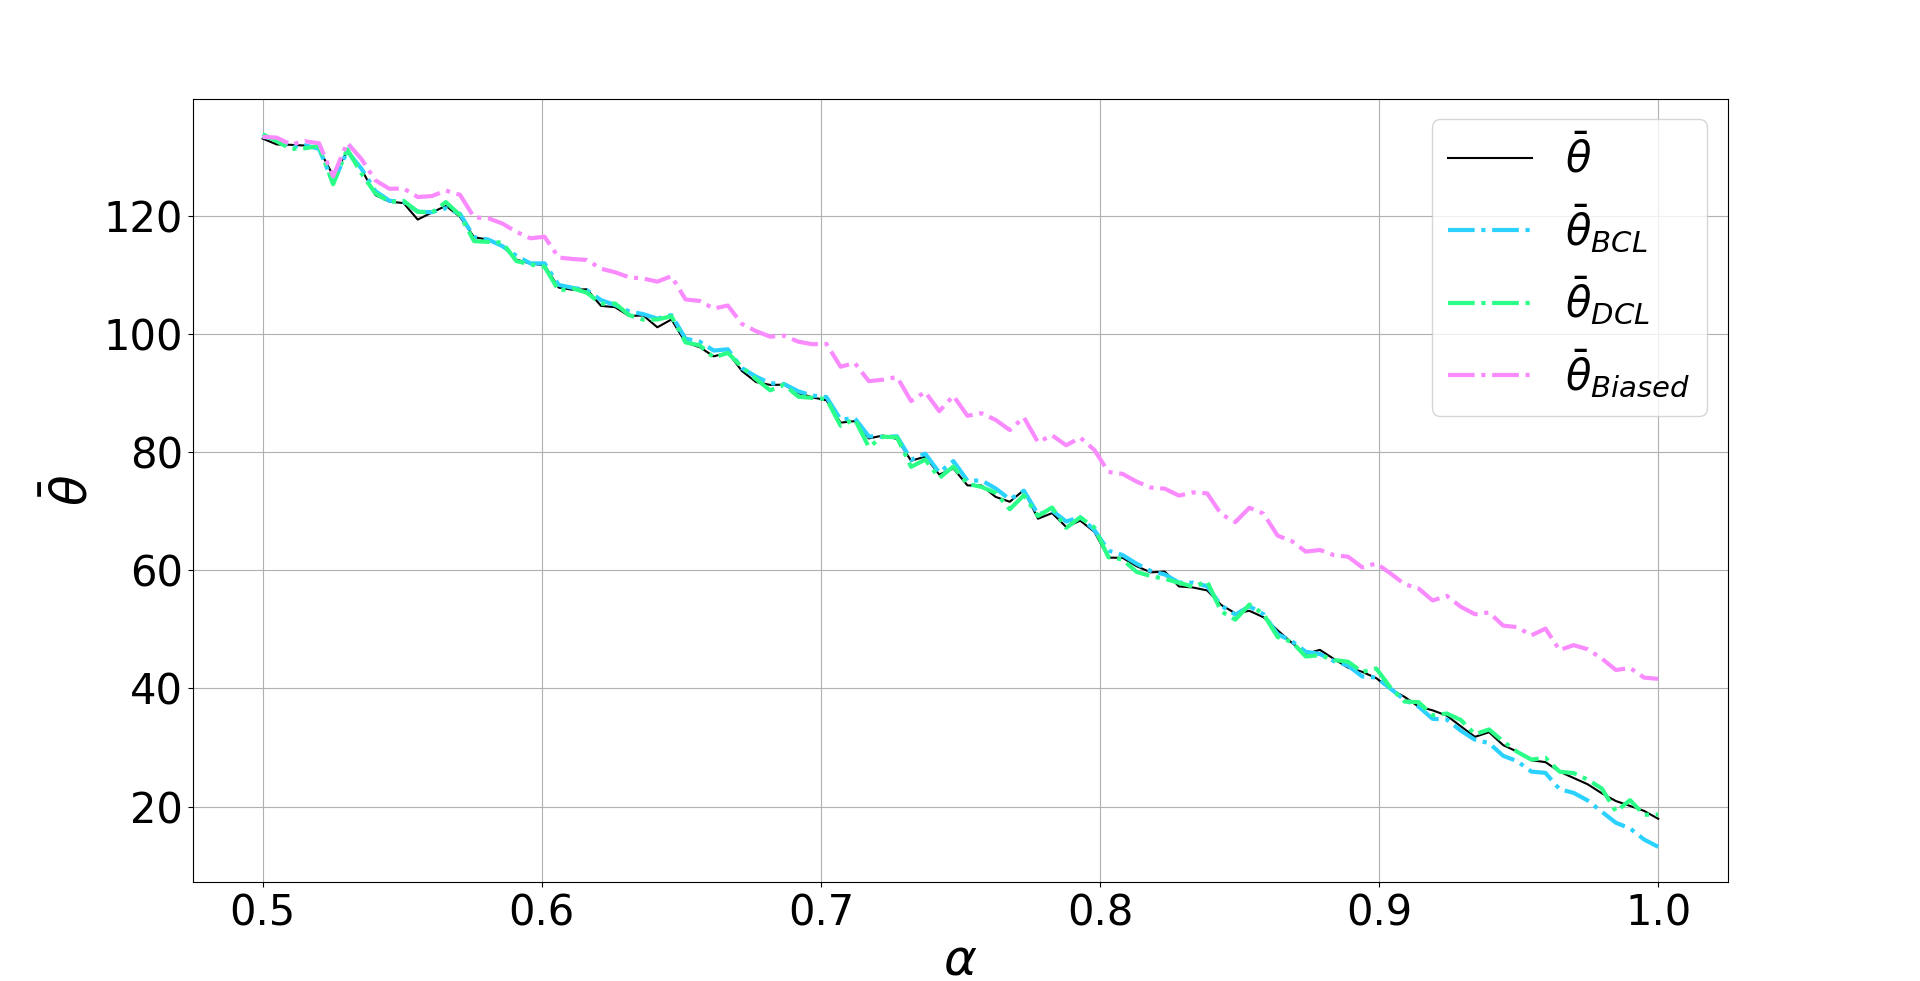
\includegraphics[width=0.49\textwidth, height=0.3\hsize]{numer_bar.png}\label{fig:numerbar_alpha}}
	\caption{不同参数设置下估计量的均值比较}
	\label{fig:numer_bar}
\end{figure}
%*******************************

\subsubsection{实验结果}
对于第$m$个锚点,可以计算得到真负例分数均值的真值,记为$\theta_{\textsc{Sup}, m}$;然后按照对比方法计算一个真负例分数的估计值,记为$\hat{\theta}_{m}$。进而,对于$M$个锚点,可以计算估计量的均方误差:
\[\textsc{Mse}\hat{\theta} = \frac{1}{M}\sum_{m=1}^M (\hat{\theta}_{m} -\theta_{\textsc{Sup}, m})^2 \]
首先固定参数设置如下:$\alpha=0.9$,$\gamma=0.1$,$\tau^+=0.1$,温度缩放$t=0.5$,锚点数量$M=1e3$,负样本数量$N=64$。然后变动不同的参数,统计不同估计量的均方误差。图\ref{Fig:MSE}对不同参数下不同估计量的均方误差MSE进行了比较。可以观察到,在不同的参数设置下,$\hat{\theta}_{\textsc{Bcl}}$估计量相对于其它估计量具有更低的均方误差。DCL方法主要受制于额外正样本得个数,在实践中,通常只有非常有限得额外正例个数可供使用。需要重点关注的是,随着负例个数N的增大,$\hat{\theta}_{\textsc{Bcl}}$的均方误差变小,与前面的分析一致。

除了MSE之外,图~\ref{fig:numerbar_alpha}还报告了不同估计量$\hat\theta$的均值在不同参数下的变化。受限于篇幅,重点关注分布$\phi$或编码器$f$的选择是否会影响估计器的一致性。图~\ref{fig: numerbar_gamma}显示了$\phi$变异对均值的影响。图~\ref{fig:numerbar_alpha}显示了编码器性能对均值的影响。
可以看到,$\hat\theta_\textsc{~Bcl}$、$\hat\theta_\textsc{~Dcl}$和$\theta$序列的均值非常接近,这是由切比雪夫大数定律保证的,即,当$\mathbb E ~\hat\theta_m = \theta_m$时,$\lim\limits_{M\rightarrow\infty} \mathbb{P}\{|\frac{1}{M}\sum_{m=1}^{M} \hat{\theta}_m-\frac{1}{M}\sum_{m=1}^{M} \theta_m |< \epsilon \} =1
$。这个结论不受建议分布$\phi$或编码器$f$的选择影响。$\hat\theta_\textsc{~Bcl}$、$\hat\theta_\textsc{~Dcl}$都是真负例分数均值的无偏估计量,这是重要性采样的性质以及均值估计量的性质决定的。此外,图\ref{fig:numerbar_alpha}也可以看作是训练过程的模拟:性能更好的编码器,即更高的$\alpha$,将真负样本编码得与锚点不相似(相似度分数更小),将正例编码得与锚点更近(相似度分数更大)。因此,观察到真负例分数均值$\bar\theta$的减少,对应于训练过程中损失值的减少,以及偏差$|\bar\theta_\textsc{Biased} -\bar\theta|$的增加,因为随着$\alpha$的增加,$\bar\theta_\textsc{Biased}$中包含的伪负样本得分更高。



\subsection{个性化推荐}
\subsubsection{数据集}
在个性化推荐任务上,与第\ref{cha:fourthsection}章相同的五个公开数据集:MovieLens-100k,MovieLens-1M,Yahoo!-R3,Yelp2018和Gowalla。数据预处理方法也一样:前三个数据集包含用户评分,按照~\cite{Steffen:2009:UAI,Zhang:2013:SIGIR,Steffen:2014:WSDM} 的方法将所有有评分的物品转换为隐式反馈。对于每个数据集,随机将其中20\%的数据作为测试数据,剩下的80\%用于训练。数据集的统计信息如表\ref{5Table:Dataset-1}所示。
\begin{table*}[h!]
	\centering
	\small
	\caption{数据集统计信息}\label{5Table:Dataset-1}
	\begin{tabular}{lrrrrrr}
		\toprule[1.2pt]
		数据集          & 用户数  & 物品数  &总交互数 & 训练集交互数  &测试集交互数&密度 \\ \cline{1-7}
		MovieLens-100k   &   943    &  1,682   &100,000&    80k	   & 20k &0.06304\\
		MovieLens-1M    &   6,040  &  3,952   &1,000,000&  800k     & 200k&0.04189  \\
		Yahoo!-R3       &   5,400  &  1,000  &182,000 &   146k      & 36k&0.03370\\
		Yelp2018       &   31,668  &  38,048&   1,561,406&   1,249k     & 312k&0.00130  \\
		Gowalla       &   29,858 &  40,981  &1,027,370 &   821k     & 205k&0.00084 \\
		\bottomrule[1.2pt]
	\end{tabular}
\end{table*}
\subsubsection{对比算法}
由于本章的出发点是通过对负样本加权,以纠正对比损失的优化目标偏差。因此使用两个具有代表性的编码器MF和LightGCN,以考察BCL损失在不同编码器上的适用性。对比方法以推荐算法中广泛使用的InfoNCE损失为基准,并进一步地选择了针对伪负例去偏任务和硬负例挖掘任务的代表性对比损失函数如下:

\begin{itemize}
	\item InfoNCE~\cite{Oord:2018:arxiv}(arXiv, 2018):InfoNCE损失是BPR损失向多个负例的推广,也是机器学习领域中最广泛使用的损失函数。在推荐领域中,优化InfoNCE损失将导致排序列表的NDCG指标的优化\cite{Jiancan:2022:arxiv}。InfoNCE损失具体表达式见式\eqref{Eq:BiasLoss},正例相似度得分通过用户和以交互物品的特征表示计算得到,负例相似度得分通过用户和其未交互物品的特诊表示计算得到。由于未交互物品中存在用户潜在感兴趣的伪负例,此时InfoNCE损失与有监督的对比损失存在偏差。
	\item DCL~\cite{Chuang:2020:NIPS}(NeurIPS Spotlight, 2020): 仅替换InfoNCE损失为DCL损失。由于未标记数据中存在伪负例,DCL提出了一个估计量见式\eqref{5Eq:DCLEstimator}来修正InfoNCE损失分母中的第二项中真负例分数和的估计。 
	\item HCL~\cite{Robinson:2021:ICLR}(ICLR, 2021): 仅替换InfoNCE损失为HCL损失。HCL损失在DCL的去偏框架的基础上,进一步使用每个随机选择的未标记样本的相似度分数加权进行困难样本挖掘。DCL是$\beta=0$时HCL的一个特例。
\end{itemize}
这些对比算法的含义在上一章实验部分已有介绍,不再赘述。

\subsubsection{超参数设置}

本章使用两种经典的推荐模型,包括经典的矩阵分解(Matrix Factorization,MF)\cite{Koren:2009:Computer},以及轻量级图卷积神经网络(LightGCN)\cite{Xiangnan:2020:SIGIR}。为了公平比较,对于所有对比算法,推荐模型的参数相同。具体参数为:(a) MF:学习率对于所有的模型和数据集都固定为$1e-3$;正则化常数:在100K和Yahoo!-R3数据集上为$1e-5$,在1M数据集上为$1e-6$,在Gowalla和Yelp2018上分别为$1e-8$; 嵌入维度:在100K数据集上为32,在1M和Yahoo!-R3数据集上为64,在Gowalla和Yelp2018上分别为128; 正例类先验$\tau^+$:在100K, 1M和Yahoo!-R3三个数据集是都设置为数据集的密度,在Gowalla和Yelp2018数据集上,由于密度太低,正例类先验都设定为$1e-2$。(b) LightGCN~\cite{Xiangnan:2020:SIGIR}:学习率、正则化常数、正例类先验概率$\tau^+$与矩阵分解模型设置一样;LightGCN层数:在100K,1M和Yahoo!-R3数据集上为1,在Gowalla和Yelp2018上设定为2;负例个数N在100K、Yahoo!-R3和1M数据集上为4,在Gowalla和Yelp2018数据集上分别为6。

对于上述两个推荐模型,BCL的去偏参数$\alpha$:在100K、1M数据集上为0.8,在Yahoo!-R3、Gowalla和Yelp2018上分别为0.7;BCL的硬负例挖掘参数$\beta$都设定为1。训练轮数固定为100,都由Pytorch实现。
100K,1M和Yahoo!-R3三个数据集的计算是在一台运行Windows 10操作系统的个人计算机上进行的,该计算机配备了2.1 GHz的CPU、一张RTX 1080Ti GPU(11GB 显存)和32 GB的RAM。Gowalla和Yelp2018两个数据集的计算是在一台运行Linux操作系统的云服务器上进行的,该服务器配备了一颗Xeon(R) Platinum 8358P CPU、一张RTX A40 GPU(40GB 显存)和56GB的RAM。

为了评估推荐的性能,采用常用的指标来评估Top-K推荐,这些指标包括精确度(Precision)、召回率(Recall)和归一化折损累积增益(NDCG),其中K的取值为5、10和20。由于这些指标的广泛使用,不在此处提供它们的定义,详细的定义请参考\cite{ml:2018}。

\subsubsection{实验结果及分析}
\begin{table*}[h!]
	\centering
	\caption{Top-k推荐性能比较}\label{5Table:Recommendation}
	\resizebox{1\textwidth}{!}{
		\begin{tabular}{lllccccccccccc}
			\toprule[1.2pt]
			\multirow{2}*{\textbf{数据集}} & \multirow{2}*{\textbf{模型}} & \multirow{2}*{\textbf{学习算法}} & \multicolumn{3}{c}{Top-5评估} &~& \multicolumn{3}{c}{Top-10评估}&~&\multicolumn{3}{c}{Top-20评估}\\ \cline{4-6} \cline{8-10} \cline{12-14}
			~ & ~ & ~ & Precision& Recall& NDCG& ~ &Precision& Recall& NDCG& ~ &Precision& Recall& NDCG \\ \hline
			
			\multirow{12}*{\textbf{MovieLens-100k}} & \multirow{6}*{\textbf{MF}} &  InfoNCE  &0.4081 & 0.1388 & 0.4324 & ~ & 0.3452 & 0.2266 & 0.4095 & ~ & 0.2793 & 0.3497 & 0.4118 \\
			~ & ~ & DCL &0.4168 & 0.1434 & 0.4458 & ~ & 0.3513 & 0.2291 & 0.4202 & ~ & 0.2835 & 0.3546 & 0.4207 \\ 
			~ & ~ & HCL  & 0.4263 & 0.1463 & 0.4539 & ~ & 0.3565 & 0.2323 & 0.426 & ~ & 0.2849 & 0.3564 & 0.4242 \\	
			~ & ~ &DPL    &\underline{0.4348} & \underline{0.1523} & \underline{0.4643} & ~ & \underline{0.3635} & \underline{0.2379} & \underline{0.4356} & ~ & \underline{0.2914} & \underline{0.3588} &\underline{0.4338} \\
			~ & ~ &BCL(proposed)    &\textbf{0.4374} & \textbf{0.1552} & \textbf{0.4674} & ~ & \textbf{0.3658} & \textbf{0.2405} & \textbf{0.4380} & ~ & \textbf{0.2931} & \textbf{0.3588} & \textbf{0.4357} \\ 
			\cline{2-14}
			
			~ & \multirow{6}*{\textbf{LightGCN}}  & InfoNCE & 0.3924 & 0.1343 & 0.4209 & ~ & 0.3349 & 0.2183 & 0.4006 & ~ & 0.2679 & 0.3289 & 0.3976 \\ 
			~ & ~ & DCL & 0.3962 & 0.1367 & 0.4243 & ~ & 0.3361 & 0.2194 & 0.4022 & ~ & 0.2695 & 0.3329 & 0.4006 \\ 
			~ & ~ & HCL & 0.4197 & 0.1461 & 0.4501 & ~ & 0.3458 & 0.2256 & 0.4188 & ~ & 0.2802 & 0.3446 & 0.4182 \\
			~ & ~ & DPL & \underline{0.4333} & \underline{0.1486} & \underline{0.4627} & ~ & \underline{0.3596} & \underline{0.2344} & \underline{0.4324} & ~ & \underline{0.2919} & \underline{0.3585} & \underline{0.4331} \\ 
			~ & ~ & BCL(proposed) & \textbf{0.4366} & \textbf{0.1512} & \textbf{0.4652} & ~ & \textbf{0.3626} & \textbf{0.2367} & \textbf{0.4351} & ~ & \textbf{0.2936} & \textbf{0.3599} & \textbf{0.4347} \\ \hline\hline
			
			
			\multirow{12}*{\textbf{MovieLens-1M}} & \multirow{6}*{\textbf{MF}} & InfoNCE & 0.3820 & 0.0879 & 0.4003 & ~ & 0.3339 & 0.1478 & 0.3728 & ~ & 0.2821 & 0.2358 & 0.3605 \\ 
			~ & ~ & DCL &  0.4009 & 0.0934 & 0.4209 & ~ & 0.3472 & 0.1546 & 0.3894 & ~ & 0.289 & 0.2423 & 0.3731\\ 
			~ & ~ & HCL & 0.4112 & 0.0969 & 0.4317 & ~ & 0.3552 & 0.1585 & 0.3991 & ~ & 0.2959 & 0.2475 & 0.3825 \\ 
			~ & ~ & DPL& \underline{0.4212} & \underline{0.0998} & \underline{0.4407} & ~ & \underline{0.3624} &\underline{ 0.1625} & \underline{0.4071} & ~ &\underline{ 0.2991} & \underline{0.2518} & \underline{0.3891} \\ 
			~ & ~ & BCL(proposed) & \textbf{0.4249} & \textbf{0.1041} & \textbf{0.4439} & ~ & \textbf{0.3652 }&\textbf{ 0.1657} & \textbf{0.4101} & ~ & \textbf{0.3012} & \textbf{0.2537} & \textbf{0.3920} \\
			\cline{2-14}
			~ & \multirow{6}*{\textbf{LightGCN}} & InfoNCE & 0.4101 & 0.0986 & 0.4386 & ~ & 0.359 & 0.1594 & 0.4041 & ~ & 0.2979 & 0.2482 & 0.3869 \\ 
			~ & ~ & DCL & 0.4104 & 0.0982 & 0.4291 & ~ & 0.3544 & 0.1597 & 0.3977 & ~ & 0.2965 & 0.2511 & 0.3842 \\ 
			~ & ~ & HCL & 0.4107 & 0.0948 & 0.4300 & ~ & 0.3514 & 0.1542 & 0.3950 & ~ & 0.2916 & 0.2413 & 0.3775 \\ 
			~ & ~ & DPL & \underline{0.4217} &\underline{ 0.1003} & \underline{0.4429} & ~ & \underline{0.3620} & \underline{0.1625} & \underline{0.1866} & ~ & \underline{0.2989} & \underline{0.2511}& \underline{0.3896} \\
			~ & ~ & BCL(proposed) & \textbf{0.4256} &\textbf{ 0.1047} &\textbf{ 0.4460} & ~ & \textbf{0.3651 }& \textbf{0.1658} & \textbf{0.1893} & ~ & \textbf{0.2998} &\textbf{ 0.2534}& \textbf{0.3911} \\\hline \hline
			
			\multirow{12}*{\textbf{Yahoo!-R3}} & \multirow{6}*{\textbf{MF}} &  InfoNCE & 0.1429 & 0.1065 & 0.1615 & ~ & 0.1080 & 0.1601 & 0.1664 & ~ & 0.0786 & 0.2316 & 0.1952 \\ 
			~ & ~ & DCL &0.1454 & 0.1083 & 0.1635 & ~ & 0.1091 & 0.1618 & 0.1692 & ~ & 0.079 & 0.2327 & 0.1974  \\ 
			~ & ~ & HCL & 0.1460 & 0.1079 & 0.1638 & ~ & 0.1096 & 0.1628 & 0.1697 & ~ & 0.0792 & 0.2336 & 0.1976 \\ 
			~ & ~ & DPL & \underline{0.1491}& \underline{0.1091} & \underline{0.1652} & ~ & \underline{0.1108} & \underline{0.1641} & \underline{0.1712} & ~ & \underline{0.0801} & \underline{0.2351} & \underline{0.2012} \\ 
			~ & ~ & BCL(proposed) & \textbf{0.1529}& \textbf{0.1122} & \textbf{0.1685} & ~ & \textbf{0.1124 }& \textbf{0.1667} & \textbf{0.1736} & ~ & \textbf{0.0815} & \textbf{0.2367} & \textbf{0.2029} \\
			\cline{2-14}
			~ & \multirow{6}*{\textbf{LightGCN}} & InfoNCE & 0.1417 & 0.1074 & 0.1676 & ~ & 0.1099 & 0.1633 & 0.1719 & ~ & 0.0798 & 0.2354 & 0.2007  \\ 
			~ & ~ & DCL & 0.1456 & 0.1092 & 0.1642 & ~ & 0.1089 & 0.1622 & 0.1697 & ~ & 0.079 & 0.2333 & 0.1982\\ 
			~ & ~ & HCL & \underline{0.1512} & \underline{0.1119} & \underline{0.1718} & ~ & 0.1130 & 0.1683 & 0.1766 & ~ & 0.0812 & 0.2394 & 0.2049 \\ 
			~ & ~ & DPL & 0.1504 & 0.1111 &  0.1706 & ~ & \underline{0.1131} & \underline{0.1670}  & \underline{0.1757} & ~ & \underline{0.0825} & \underline{0.2412} & \underline{0.2054}\\ 
			~ & ~ & BCL(proposed) & \textbf{0.1537} & \textbf{0.1140} &  \textbf{0.1725} & ~ & \textbf{0.1156} & \textbf{0.1696}  & \textbf{0.1771} & ~ & \textbf{0.0842} & \textbf{0.2428} & \textbf{0.2076}\\ \hline\hline
			
			
			\multirow{12}*{\textbf{Yelp2018}} & \multirow{6}*{\textbf{MF}} & InfoNCE  & 0.0429 & 0.0246 & 0.047 & ~ & 0.0365 & 0.0417 & 0.0491 & ~ & 0.0305 & 0.07 & 0.058 \\ 
			~ & ~ & DCL & 0.0486 & 0.0278 & 0.0531 & ~ & 0.0410 & 0.0466 & 0.0552 & ~ & 0.0342 & 0.0777 & 0.0648 \\
			~ & ~ & HCL & 0.0515 & 0.0305 & 0.0566 & ~ & 0.0459 & 0.0541 & 0.0622 & ~ & 0.0383 & 0.0894& 0.0736 \\ 
			~ & ~ & DPL & \underline{0.0543} & \underline{0.0325} & \underline{0.0595} & ~ & \underline{0.0463} & \underline{0.0551} & \underline{0.0630} & ~ & \underline{0.0389} & \underline{0.0914} & \underline{0.0749} \\
			~ & ~ & BCL(proposed) & \textbf{0.0566} &\textbf{ 0.0362} & \textbf{0.0615} & ~ & \textbf{0.0475} &\textbf{ 0.0581} & \textbf{0.0663} & ~ & \textbf{0.0409} & \textbf{0.0942} & \textbf{0.0773} \\
			\cline{2-14}
			~ & \multirow{6}*{\textbf{LightGCN}} & InfoNCE & 0.0553 & 0.0329 & 0.0607 & ~ & 0.0473 & 0.0558 & 0.0642 & ~ & 0.0390 & 0.0911 & 0.0754 \\ 
			~ & ~ & DCL & 0.0559 & 0.0331 & 0.0612 & ~ & 0.0472 & 0.0557 & 0.0642 & ~ & 	0.0391 & 0.0914 & 0.0756 \\ 
			~ & ~ & HCL & 0.0563 & 0.0335 & 0.0617 & ~ & 0.0477 & 0.0564 & 0.0648 & ~ & 0.0393 & 0.0920 & 0.0760 \\  
			~ & ~ & DPL & \underline{0.0604} & \underline{0.0364} &\underline{0.0657} & ~ & \underline{0.0513} & \underline{0.0615} & \underline{0.0696} & ~ &\underline{0.0423} & \underline{0.1003} & \underline{0.0821} \\
			~ & ~ & BCL(proposed) & \textbf{0.0642} & \textbf{0.0398} & \textbf{0.0696} & ~ & \textbf{0.0554} & \textbf{0.0656} &\textbf{ 0.0729} & ~ & \textbf{0.0442} & \textbf{0.1045} & \textbf{0.0847} \\\hline\hline
			
			
			\multirow{12}*{\textbf{Gowalla}} & \multirow{6}*{\textbf{MF}} & InfoNCE & 0.0739 &0.0757 & 0.1016 & ~ & 0.0560 & 0.1122 & 0.1076 & ~ & 0.0422 & 0.1650 & 0.1230\\ 
			~ & ~ & DCL & 0.0746 & 0.0769 &0.1023 & ~ & 0.0568 & 0.1147 & 0.1088 & ~ & 0.0426 & 0.1664 & 0.1238 \\ 
			~ & ~ & HCL & 0.0755 & 0.0774 & 0.1035 & ~ & 0.0574 & 0.1151 & 0.1098 & ~ & 0.0432& 0.1693 & 0.1256 \\ 
			~ & ~ & DPL & \underline{0.0815} & \underline{0.0827} & \underline{0.1100} & ~ & \underline{0.0628} & \underline{0.1243}& \underline{0.1174} & ~ & \underline{0.0473} & \underline{0.1815} & \underline{0.1340} \\
			~ & ~ & BCL(proposed) & \textbf{0.0827} & \textbf{0.0837} & \textbf{0.1121} & ~ & \textbf{0.0639} & \textbf{0.1257}& \textbf{0.1186} & ~ & \textbf{0.0485} & \textbf{0.1824} & \textbf{0.1353} \\
			\cline{2-14}
			~ & \multirow{6}*{\textbf{LightGCN}} &  InfoNCE & 0.0743 & 0.0760 & 0.1022 & ~ & 0.0566 & 0.1132& 0.1084 & ~ & 0.0423 & 0.1649 & 0.1231\\ 
			~ & ~ & DCL & 0.0748 & 0.0763 & 0.1027 & ~ & 0.0569 & 0.1132 & 0.1088 & ~ & 0.0424 & 0.1656 & 0.1236 \\ 
			~ & ~ & HCL & 0.0852 & 0.0874 & 0.1156 & ~ & 0.0658 &0.1321 & 0.1237 & ~ & \underline{0.0495} & 0.1930 & \underline{0.1409} \\ 
			~ & ~ & DPL &  \underline{0.0867} &   \underline{0.0891} &  \underline{0.1164} & ~ &  \underline{0.0662} &  \underline{0.1329} & \underline{0.1242} & ~ &  0.0494 &  \underline{0.1936} &  0.1407 \\ 
			~ & ~ & BCL(proposed) & \textbf{0.0893} & \textbf{ 0.0923} & \textbf{0.1203} & ~ &  \textbf{0.0690} &  \textbf{0.1372} & \textbf{0.1288} & ~ & \textbf{0.0502} &\textbf{ 0.1987} & \textbf{0.1476}  \\\hline
			\bottomrule[1.5pt]
			
		\end{tabular}
	}
\end{table*}

表\ref{5Table:Recommendation}对比了不同的学习算法在五个数据集上的top-k评估结果。可以看到BCL算法在不同数据集的所有top-k评估指标上取得了一致的最优,验证了BCL方法的伪负例去偏和硬负例挖掘的有效性。其次,有去偏机制的DCL, HCL, BCL, DPL表现普遍优于没有去偏机制的InfoNCE,尤其是在密度较高的数据集上有去偏机制的学习算法优势更明显,说明在密度较大(伪负例率较高)的场景进行伪负例去偏的重要性。第三,包含硬负例挖掘机制的HCL方法和BCL方法普遍优于不含硬负例挖掘机制的DCL和InfoNCE方法。在个性化推荐场景中,伪负例率普遍较低,含有硬负例挖掘机制的学习算法优势较为突出,说明硬负例挖掘机制的重要性。

需要着重强调的是HCL和BCL的差别,它们都包含困难负例挖掘和伪负例去偏机制,但是BCL优于HCL方法。这是由于两者重要性加权机制的不同所造成的:HCL的权重可以简单理解为未标注样本相似度分数的指数次方,相似度分数越大,重要性权重越大,可以很好地实现硬负例挖掘任务,但无法兼顾伪负例去偏任务;BCL的权重是未标注样本是真负例的后验概率,可以灵活地兼顾硬负例挖掘和伪负例去偏任务。此外,HCL的权重是样本相似度分数的函数,而BCL的权重是经验分布函数(相对排序位置)的函数。在推荐中,嵌入倾向于过度平滑,从而导致相似度分数趋同,那么HCL的权重可能会消失。而BCL的权重不会受到相似度分数具体值的影响,因此表现出了更好的鲁棒性。

\subsection{图像分类}
BCL虽然针对对比型推荐算法在自监督设置下的优化目标偏离问题设计,但是这一问题具有普遍性。考虑到InfoNCE对比损失的广泛使用,额外考虑无监督图像分类任务以验证BCL损失的有效性。

图像分类任务与个性化推荐任务类似,都是通过优化对比损失预训练模型学习样本的表示,根据学到的表示进行下游排序或者分类任务。以SimCLR\cite{Chen:2020:ICML}框架为例,其对比损失的计算方式为:同一个样本的两次增强的特征表示构成正样本对,得到正例相似度得分;该样本与其它未标注的样本的特征表示构成负样本对,得到负例相似度得分。尽管下游任务的评估协议略有差异:推荐任务是根据用户表示的K近邻物品表示生成top-K推荐(即内积相似度高的物品);图像分类任务是将学到的表示固定,然后训练一个线性分类器。但共同点是,学到的对比表示质量越好,即正例越对齐,负例越均匀,下游排序或者分类任务的泛化性能越好\cite{Arora:2019:ICML}。
\subsubsection{数据集}
在图像分类任务上,使用了四个公开数据集,CIFAR10,STL10,CIFAR100和tinyImageNet数据集。简单介绍CIFAR10数据集,CIFAR-10数据集包含10个类别的60000张尺寸为32x32的彩色图像,每个类别有6000张图像。其中,训练集包含50000张图像,测试集包含10000张图像。不同类别的训练样本完全互斥,且类别平衡。图\ref{Fig:cifar}提供了CIFAR10数据集的十个类别及相应的随机样本概览。其余三个数据集与CIFAR10数据集类似,都是类别平衡。除了STL10数据集以外,其他数据集都是完全标注的,但在训练过程中,都不使用训练集的样本的类别标签,仅在评估的时候使用类别标签。这四个数据集的统计信息如下表:
\begin{figure}[h!]
	\centering
	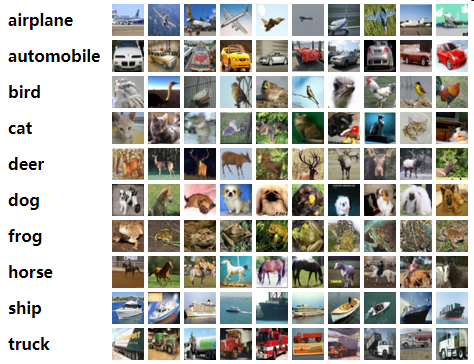
\includegraphics[width=0.7\textwidth]{cifar.png}
	\caption{CIFAR10数据集的十个类别及相应的随机样本概览}
	\label{Fig:cifar}
\end{figure}
\begin{table*}[h!]
	\centering
	\small
	\caption{图像多分类任务数据集统计信息}\label{5Table:Dataset}
	\resizebox{1\textwidth}{!}{
		\begin{tabular}{lcccccc}
			\toprule[1.2pt]
			数据集          & 类别总数  & 图像尺寸  &训练集数量  &验证集数量&测试集数量&是否完全标注   \\ \cline{1-7}
			CIFAR10   &   10    &  32x32(RGB)   &50,000&   /	   & 10,000 &是\\
			STL10    &   10  &  96x96(RGB)  &105,000&  /     & 8,000&否  \\
			CIFAR100       &   100 &  32x32(RGB)  &50,000 &  /      & 10,000&是\\
			tinyImageNet       & 200&  64x64(RGB) &  100,000&   10,000&    10,000    & 是 \\
			\bottomrule[1.2pt]
		\end{tabular}
	}
\end{table*}

此外,在正例类先验概率比较高的场景下,不同算法的表现是衡量去偏性能的一个重要标准。在上述数据集中,随机选定两个类别的所有样本,构造了新的二分类数据集,统计信息如表\ref{6Table:Dataset}所示。在二分类数据集中,对于一个锚点,随机的未标注样本中,与锚点同类(伪负例)的概率为50\%。其中,STL10数据集中,有标记的数据集合计5000张,二分类数据集从已标记的样本中选取。
\begin{table*}[h!]
	\centering
	\small
	\caption{图像二分类任务数据集统计信息}\label{6Table:Dataset}
	\resizebox{\textwidth}{!}{
		\begin{tabular}{lcccccc}
			\toprule[1.2pt]
			数据集           & 类别总数 & 图像尺寸  &训练集数量  &验证集数量&测试集数量&是否完全标注   \\ \cline{1-7}
			CIFAR10   &   2    &  32x32(RGB)   &10,000&   /	   & 2,000 &是\\
			STL10    &   2  &  96x96(RGB)  &1,000&  /     & 1600 &是 \\
			CIFAR100       &   2&  32x32(RGB)  &1,000 &  /      & 200&是\\
			tinyImageNet       & 2&  64x64(RGB) &  1,000&  100&    100    &是\\
			\bottomrule[1.2pt]
		\end{tabular}
	}
\end{table*}

\subsubsection{对比方法}
BCL通过对未标注样本进行加权,从而校准负例的梯度,不适用于两个网络分支分别采用梯度法和动量法更新的异步网络架构,因此主要考虑以SimCLR\cite{Chen:2020:ICML}为代表的端到端梯度下降的对比学习算法。固定编码器为ResNet50,其它对比方法具体如下:
\begin{itemize}
\item SimCLR\cite{Chen:2020:ICML}(ICML, 2020): 该方法包含4个关键组件,分别为随机数据增强模块、ResNet-50编码器,神经网络投影头,以及InfoNCE对比损失。由于训练时不使用样本标签,in-batch内的未标注样本被当作负例以计算对比损失,从而导致对比损失优化目标的偏离。

\item DCL\cite{Chuang:2020:NIPS}(NeurIPS Spotlight, 2020): 该方法沿用SimCLR的框架,仅修改对比损失为DCL损失进行伪负例去偏。

\item HCL\cite{Robinson:2021:ICLR}(ICLR, 2021): 该方法沿用SimCLR的框架,仅修改对比损失为HCL损失进行硬负例挖掘。
\end{itemize}
由于在图像数据集上较小的负例个数N导致性能的显著下降,在图像分类任务上不考虑上一章的负例个数为1的DPL对比算法。

\subsubsection{超参数设置}
实验设置与DCL~\cite{Chuang:2020:NIPS}和HCL~\cite{Robinson:2021:ICLR}完全相同,仅损失函数不同,以进行公平的比较。具体而言,所有的对比方法使用完全相同的数据增强方法,使用ResNet-50\cite{He:2016:CVPR}作为编码器架构,并使用学习率为0.001的Adam优化器~\cite{Adam:2015:ICLR}。温度缩放系数和潜在向量的维度分别固定为$t$=0.5和$d$=128。以24GB显存的RTX3090显卡为例,能够承受的最大的N=510,此时批量大小为256(在SimCLR框架下,负例个数N=2 $\times$ batch\_size -2)。固定负例个数N=510,所有模型训练400个轮次。关于BCL方法的去偏参数和硬负例挖掘参数,在CIFRA10数据集上,$\alpha$是通过经验评估计算的,$\beta=0.9$;在STL10数据集上,设定$\alpha=0.75$,$\beta=1.0$;在STL10数据集上,设定$\alpha=0.7$,$\beta=1.0$;在TinyImageNet数据集上,设定$\alpha=0.8$,$\beta=1.0$。类先验概率$\tau^+$都设定为$1/C$,其中$C$为数据集的类别总数。


在评估上与推荐任务有所不同,图像分类任务的评估遵循已有的评估协议:首先固定学习到的嵌入,然后通过训练线性分类器进行评估~\cite{Lajanugen:2018:ICLR,Robinson:2021:ICLR},评估指标使用ACC\cite{ml:2018}。在训练时均不使用标签,只在评估时使用样本标签。


\subsubsection{实验结果及分析}
表\ref{Exp:acc}展示了多分类任务的实验结果。第一个观察结果是,本章提出的BCL取得了最优的表现。方法BCL相对于对于SimCLR,top-1分类精度分别取得了1.4%,7.3%,3.3%和3.9%的绝对提升。相对于次优方法HCL,BCL的top-1分类精度分别取得了0.6%,0.1%,0.2%和0.3%的绝对提升,在CIFAR10和TinyImagenet数据集上的提升具有显著性。
第二个观察结果是,注重硬负例挖掘的HCL通常取得次优表现(CIFAR10数据集除外),明显优于SimCLR和DCL。类别较多意味着较低的伪负例率。HCL优于DCL说明,\textbf{在伪负例率较低的场景,硬负例挖掘比伪负例去偏更重要}。第三个观察结果是,具有去偏机制的DCL优于没有去偏机制的SimCLR方法,说明即使在伪负例率较低的场景,伪负例去偏也会带来性能提升。
\begin{table}[h!]
	\centering
	\caption{图像多分类top-1精度比较}\label{Exp:acc}
	\resizebox{0.8\textwidth}{!}{
		\begin{tabular}{lcccccc}
			\toprule[1.2pt]
			
			数据集&负例个数N &模型& SimCLR & DCL & HCL & \textbf{BCL}  \\ \hline
			CIFAR10 & 510 &ResNet50& 91.1   & \underline{92.1}	&91.9	&\textbf{92.5}($\pm 0.15$) \\
			STL10& 510 &ResNet50& 80.2   &84.3	&\underline{87.4}	&\textbf{87.5}($\pm 0.12$)\\
			CIFAR100& 510&ResNet50 & 66.4   &67.7	&\underline{69.5}	&\textbf{69.7}($\pm 0.10$)\\
			tinyImageNet& 510&ResNet50 & 53.4   &53.7	&\underline{57.0}	&\textbf{57.3}($\pm 0.09$)\\
			\cline{1-7}
			\bottomrule[1.2pt]
			
		\end{tabular}
	}
\end{table}

表\ref{Exp:result2}展示了二分类任务的实验结果。第一个观察结果是,本章提出的BCL取得了最优的表现。在二分类任务上,BCL相对于对于SimCLR,top-1分类精度分别取得了0.2%,1.0%,1.2%和2.0%的绝对提升。相对于HCL,BCL的top-1分类精度分别取得了0.9%,1.6%,2.3%和5.0%的绝对提升。第二个观察结果是,在二分类任务上,次优方法通常是SimCLR取得的的,而DCL和HCL的表现不佳。这并不是伪负例去偏机制和硬负例挖掘机制在伪负例率较高的二分类场景无效,而是与DCL和HCL所采用的伪负例去偏机制缺乏灵活性有关。其采用的估计量为$\hat{\theta} =  \frac{1}{N\tau^-}  (\sum_{i=1}^{N} \hat{x}_i - N\tau^+ \cdot \frac{\sum_{j=1}^{K} \hat{x}_j^+}{K} ) $,当伪负例率$\tau^+$过大,其减去项$N\tau^+ \cdot \frac{\sum_{j=1}^{K} \hat{x}_j^+}{K}$也过大,削弱了困难样本的梯度值。而BCL则不会受过大的$\tau^+$影响。第三个观察结果是,DCL表现优于HCL(CIFAR100数据集除外)。这是因为伪负例太多,即噪声率太高,过度强调困难样本的挖掘,容易使模型学到了伪负例(噪声)的错误模式,说明\textbf{在伪负例率较高的场景,伪负例去偏任务比硬负例挖掘更加重要}。


\begin{table}[h!]
	\centering
	\caption{图像二分类top-1精度比较}\label{Exp:result2}
	\resizebox{0.8\textwidth}{!}{
		\begin{tabular}{lcccccc}
			\toprule[1.2pt]
			数据集&负例个数N&编码器&	SimCLR&	DCL &	HCL&	\textbf{BCL}\\\hline
			CIFAR10&	510	&ResNet50&\underline{99.1}	&98.7&	98.4&	\textbf{99.3}($\pm 0.22$)\\
			STL10	&510&ResNet50&	\underline{91.7}&	91.2&	91.1&	\textbf{92.7}($\pm 0.34$)\\
			CIFAR100&	510&ResNet50	&\underline{97.5}&	86.9&	96.5&	\textbf{98.8}($\pm 0.28$)\\
			tinyImageNet&	510&ResNet50&	\underline{97.0}&	96.0&	94.0&\textbf{99.0}($\pm 0.25$)\\
			\cline{1-7}
			\bottomrule[1.2pt]
			
		\end{tabular}
	}
\end{table}


\subsection{超参数分析}
由于图像数据集上标注比较完备,因此使用图像数据集分析不同超参数的影响。

\textbf{负例个数N的影响}:首先固定$\alpha$和$\beta$的值如上所述,然后分析不同负例个数N对分类精度的影响。结果如表\ref{Exp:result}所示,更大的负例个数N导致了分类精度一致的提升。这与对比损失本身的性质有关,更大的N导致了更大的互信息下界。此外,对于所提出的BCL方法,更大的N导致(1)经验分布函数$\hat{\Phi}_\textsc{Un}(\hat{x})$的估计误差减小;(2) $\alpha$的估计误差减小;(3)重要性采样的估计误差减小,从而使得BCL经验估计的估计误差确定性地减小,这与数值实验部分的结论是一致的。
\begin{table}[h!]
	\centering
	\caption{负例个数的影响}\label{Exp:result}
	\resizebox{0.6\textwidth}{!}{
		\begin{tabular}{cclcccc}
			\toprule[1.2pt]
			\multirow{2}*{数据集} &  \multirow{2}*{学习算法} & \multicolumn{5}{c}{负例个数N} \\\cline{3-7}
			
			~ & ~ & N=30 & N=62& N=126& N=254&N=510 \\ \hline
			
			\multirow{2}*{\textbf{CIFAR10}} & SimCLR & 80.21 & 84.82   &87.58&89.87	&91.12\\
			~&BCL& 83.61 & 88.56   &90.83	&92.07	&92.58\\
			\cline{1-7}
			
			\multirow{2}*{\textbf{STL10}} & SimCLR & 61.20 & 71.69   &74.36	&77.33	&80.20\\
			~&BCL& 67.45 & 73.36   &80.23	&84.68	&87.51\\
			\cline{1-7}
			\bottomrule[1.2pt]
			
		\end{tabular}
	}
\end{table}


\begin{table}[h!]
	\centering
	\caption{参数$\beta$的影响}\label{Exp:beta}
	\resizebox{0.6\textwidth}{!}{
		\begin{tabular}{lclcccc}
			\toprule[1.2pt]
			
			数据集 & $\beta=0.5$ & $\beta=0.6$ & $\beta=0.7$ & $\beta=0.8$ & $\beta=0.9$ &$\beta=1.0$  \\ \hline
			\textbf{CIFAR10}&91.39 & 91.41 & 91.89   &92.02	&\textbf{92.58}	&92.12\\
			\textbf{STL10}&80.32& 81.79 & 83.58   &83.83	&84.85	&\textbf{87.51}\\
			\cline{1-7}
			\bottomrule[1.2pt]
			
		\end{tabular}
	}
\end{table}

\textbf{困难负例挖掘参数$\beta$的影响}:$\alpha$对应于当前参数下编码器的宏AUC,有明确的含义;而$\beta$控制着采样分布的难度级别(hardness level),是手动选择的,因此只分析参数$\beta$的影响。固定最优参数$\alpha$不变,然后检查不同$\beta$值的影响。表~\ref{Exp:beta}展示了难度级别$\beta$的影响。在STL10数据集上,随着$\beta$的增加,top-1分类精度持续提高。然而,在CIFAR10数据集上,随着$\beta$的增加,tip-1分类准精度逐渐增加,在0.9处达到最优值后开始下降。这结果表明,更高的难度级别并不总是导致更好的性能。这一观点也可以从HCL和DCL的性能比较得到印证,HCL(包含困难负样本挖掘机制)在CIFAR10数据集上的表现比DCL(不包含困难负样本挖掘机制)要差。

如何设定一个合理的硬负例挖掘参数$\beta$?关于深度神经网络的记忆效应的研究~\cite{Arpit:2017:ICML}为回答这个问题提供了启发。具体而言,已经证明,不论使用何种网络架构,深度模型会优先记忆带有干净标签的训练数据,并随着训练轮数的增加逐渐适应带有噪声标签的训练数据~\cite{zhang2021understanding, Han:2018:NIPS}。自监督对比学习可以被视为一个负例含有噪声的噪声标签学习(Noisy Label Learning)问题。较大的$\beta$值会导致给困难样本分配更高的权重,从而导致更大的损失值和相应的梯度值。为了避免神经网络拟合噪声,在正类先验较小的数据集(即噪声比较低的数据集)中,设置较大的$\beta$值可以加快对干净的困难样本的拟合;而在正类先验较小的场景中,应该选择一个较小的$\beta$值,从而避免拟合噪声数据。因此一个启发式的$\beta$设定值可以为
\[\beta = 1-1/C\]
其中,C为数据集的类别总数,那么1/C即为噪声率,越小的噪声率,那么应该设定一个更接近于1的$\beta$值。真是数据集的实验也验证了这个结论:在100类的CIFAR100和200类的tinyImageNet数据集上,最优的参数值为1。除了噪声率以外,另外一个需要考虑的因素是数据集本身拟合的难易度水平。与CIFAR-10数据集相比,STL-10数据集具有更大的挑战,它的top-1分类精度显著低于CIFAR10。因此,在相对难以拟合的STL-10数据集中,应当使用较大的$\beta$值可以激励神经网络在拟合噪声样本之前先拟合干净的困难样本。在相对容易拟合的CIFAR-10数据集中,应当使用相对小一点的$\beta=0.9$,避免神经网络拟合噪声样本。

\begin{table}[h!]
	\centering
	\caption{正例类先验概率$\tau^+$的影响}\label{Exp:tau}
	\resizebox{0.5\textwidth}{!}{
		\begin{tabular}{clccc}
			\toprule[1.2pt]
			数据集&	负例个数N &$\tau^+$	&	top1&	top5 \\\hline
			tinyImageNet&	510	&1e-3&	57.10&	80.54\\
			tinyImageNet&	510&	5e-3&	57.32&	80.87\\
			tinyImageNet&	510&	1e-2&	56.34&	80.24\\
			\cline{1-5}
			\bottomrule[1.2pt]
		\end{tabular}
	}
\end{table}

\textbf{$\tau^+$的影响}:表\ref{Exp:tau}展示了正例类先验概率$\tau^+$的设置对分类精度的影响。结果显示最佳的$\tau^+ = 1/C$。考虑数据集中的一个特定类别,比如"猫",可以将属于猫类的图像数量记为随机变量$X$,它可以看作N次独立成功率为$\tau^+$伯努利试验的结果,那么 $X\sim B(Y,\tau^+)$,其中$Y$是数据集中的所有样本数。在这种情况下,$\tau^+$的无偏估计$X/Y$。在一个平衡的数据集中,数据集中的总样本数为$Y = C * X$,其中$C$是类别的数量,$X$是每个类别中的样本数,于是有$\tau^+ = 1/C$。

\subsection{运行时间比较}
前面分析了,本章的方法的额外计算开销主要是由于经验分布函数的计算,其复杂度为O(N),其中N = 2 * (batch size-1),相比于编码一个样本,这个开销是可以忽略的。表\ref{Exp:time}比较了在不同数据集上进行单个训练周期的实际运行时间。其中,批量大小固定为256,编码器架构为ResNet-50。在CIFAR10、STL10和CIFAR100数据集上的实验是在配备了Intel(R) Xeon(R) Platinum 8255C CPU和单卡的RTX 3090(24GB) * 1 GPU的云服务器上进行的。在tinyImageNet数据集上的实验是在配备了Intel(R) Xeon(R) Platinum 8352M CPU和单卡的A100-SXM4-80GB(80GB) * 1 GPU的云服务器上进行的。结果显示,本章提出的方法几乎相比于对比方法有着相同的运行时间。tinyImageNet数据集运行时间较长是因为图像增强模块中,随机剪裁后图像的尺寸相对于前面三个数据集更大。
\begin{table}[h!]
	\centering
	\caption{算法运行时间比较}\label{Exp:time}
	\resizebox{0.5\textwidth}{!}{
		\begin{tabular}{llcc}
			\toprule[1.2pt]
			数据集&	Batch Size&	SimCLR&		BCL \\ \hline
			CIFAR10	&256&	82s/epoch	&	82s/epoch\\
			STL10&	256	&169s/epoch	&	169s/epoch\\
			CIFAR100&	256	&82s/epoch&	82s/epoch\\
			tinyImageNet&	256&	237s/epoch&238s/epoch\\
			\cline{1-4}
			\bottomrule[1.2pt]
		\end{tabular}
			}
\end{table}
\section{本章小结}
本章提出贝叶斯自监督对比损失,通过重要性权重来纠正从无标签数据中随机选择的负样本导致的偏差。从单个权重来看,BCL提供了样本是真负例的后验概率估计。BCL计算的权重是样本是真负例的后验概率线性函数,为真负样本赋以较大权值,遵循硬负例原则;为伪负例赋以较小的权值,遵循真负例原则。从损失函数值来看,BCL提供了有监督数据下对比损失的一致估计。通过重要性加权未标注样本相似度分数,实现对真负例相似度分数的近似,间接地实现了对有监督损失的近似,从而提升下游任务的泛化性能。其关键思想是在贝叶斯框架下推导目标采样群体的概率,该分布具有参数化结构,可以灵活统一地执行硬负例挖掘和伪负例去偏任务这两个冲突任务。在数值实验、个性化推荐、图像分类任务上验证了贝叶斯自监督对比损失的有效性,只需要简单地修改损失函数,而无需额外的存储和计算开销。

本章对前面章节方法的局限性进行了全面的考量并改进:针对第三章伪正例问题,本章解决了更具普遍性的负例无监督问题,且解决方案不再依赖于表示向量高斯分布的参数化假设,从而成功地将模型从简单的矩阵分解向图卷积神经网络和残差网络进行了推广。针对第四章显式负采样带来的额外计算开销问题,本章通过校正估计不引入额外的计算开销,与基线方法有着相同的运行时间。此外通过图\ref{Fig:openball}对正例和负例相似度分数的分析,突破了第四章所依赖的“正例分数大于负例分数”的假设,获取类条件概率密度不再依赖任何参数化的假设。针对第五章仅聚焦于单个负例的对比损失去偏,本章通过重要性权重加权将去偏目标向更具一般性的多个负例的对比损失推广;此外在伪负例去偏的基础上,进一步考虑了硬负例挖掘,综合全面地考虑了对比型推荐算法的任务需求。
